\documentclass[11pt,Chicago]{uuthesis}
\usepackage{amsfonts,amsthm,mathrsfs}
\usepackage{amsmath,amssymb}
\usepackage[mathscr]{euscript}
\usepackage{thesis}
\usepackage{graphicx}
\usepackage{subfigure}
\usepackage{latexsym}
\usepackage{flafter}
\usepackage{afterpage}
\usepackage{algorithm}
\usepackage{clrscode}
\usepackage{wrapfig}
\usepackage{multirow}
 \usepackage{booktabs}



\usepackage{color}
\usepackage[table]{xcolor}
\definecolor{darkgreen}{rgb}{0.0, 0.4, 0.0}
\definecolor{darkblue}{rgb}{0.0, 0.0, 0.6}
\definecolor{darkred}{rgb}{0.6, 0.0, 0.0}

% Make sure subfigures have parentheses around them everywhere
%\renewcommand\thesubfigure{(\alph{subfigure})}
% Make sure subfigures have parentheses around them everywhere
%\renewcommand\thesubfigure{(\alph{subfigure})}

\usepackage{lscape}
%\usepackage{diagram}
%\usepackage{tgrind}
\let \tenrm = \rm 		% This is used in fig*.tex
%\includeonly{}                    % Only front matter and back matter
%\includeonly{chap1}               %  plus chapter 1
%\includeonly{chap2}                %  plus chapter 2
%\includeonly{chap3}                %  plus chapter 3
%\includeonly{appA}                %  plus chapter 3
%\includeonly{chap1,chap2,chap3,chap4}   %  plus all chapters
%\includeonly{chap1,chap2,chap3,chap4,appA}   %  plus all chapters & appendix
%
%\tracingstats=2                % show TeX memory usage
\title{Towards the Theory and Practice of \protect\\ Verifying Visualizations}
\author{Tiago Etiene}
\thesistype{thesis} % or dissertation
\graduatedean{Graduate Dean's name}
\department{Computer Science}
\degree{Doctor of Philosophy}  % of Doctor of Philosophy
\departmentchair{First M. Last}
\committeechair{First M. Last}
\firstreader{First M. Last}
\secondreader{First M. Last}
%\thirdreader{First M. Last}
%\fourthreader{First M. Last}
\chairtitle{Professor}
\submitdate{February 2013}
\copyrightyear{2013}
% Chapter is one level, section and subsection are the next two levels.
\fourlevels
%\dedication{For my horse, Dixie, etc. A few lines only.}
 \inputpicturetrue  % By Jeff McGough. See uuguide and private thesis.sty
%\inputpicturefalse % To NOT produce pictures, uncomment this line


\theoremstyle{plain}
\newtheorem{thm}{Theorem}[section]

\theoremstyle{definition}
\newtheorem{dff}[thm]{Definition}

\DeclareMathAlphabet{\mathpzc}{OT1}{pzc}
                                 {m}{it}
                                 
\newcommand{\deliso}{$\proc{DelIso}$}
\newcommand{\mclewiner}{$\proc{MC33}$}
\newcommand{\vtk}{$\proc{VTKMC}$}
\newcommand{\afront}{$\proc{Afront}$}
\newcommand{\matlab}{$\proc{Matlab}$}
\newcommand{\macet}{$\proc{Macet}$}
\newcommand{\mcsimpleflow}{$\proc{MCFlow}$}
\newcommand{\Matlab}{$\proc{Matlab}$}
\newcommand{\snapmc}{$\proc{SnapMC}$}
\newcommand{\setitemsep}{\setlength{\itemsep}{0pt}}

\newcommand{\gc}{\rowcolor[gray]{.9}}
\newcommand{\s}{~~~~}
\newcommand{\cc}{\cellcolor[gray]{.9}}
\newcommand{\vnv}{V\&V}
\newcommand{\cs}{CS}
\newcommand{\cse}{CS\&E}
\newcommand{\mc}{\textsc{MC33}}
\newcommand{\cmc}{\textsc{C-MC33}}

\global\newcount\nn \nn=0
\def\Sen{\global\advance\nn by 1 \number\nn}
\newcommand{\bugnumber}{\Sen}

\hyphenation{Algorithms}






\begin{document}
%% Comment out items by inserting a percent % character
\frontmatterformat
\titlepage
\copyrightpage
\committeeapproval
%\readingapproval
\preface{abstract}{Abstract}
%\dedicationpage
%\begin{epigraph}
%``Nature is trying very hard to make us succeed, but nature does not depend on us. We are not the only experiment.''
%\begin{flushright} -- R. Buckminster Fuller \par\end{flushright}
%\end{epigraph}
\setcounter{tocdepth}{4}    %How many levels to include in TOC
\addtocontents{toc}{\protect\sloppy}    %Keeps long chapters within page # margins
\tableofcontents
\listoffigures
\listoftables
%
% Optional front page, made from source "notation.tex".
% If you don't need it, then don't use it.
%
%\optionalfront{Notation and Symbols}{\input{notation.tex}}
\preface{acknowledge}{Acknowledgments}
\maintext       % Start normal page numbering. Parts and chapters follow.
\chapter{Introduction}

Today's technology provide unprecedented opportunities to scientists for deriving, expanding, or correcting scientific theories. In the past few decades, we  have seen an ever increasing capability of acquire, store, and process data. Simultaneously, the scientific visualization emerged as discipline, and started to play a crucial role in the pipeline of many scientists. In fact, visualization became the means through which scientists explore, evaluate, and present results. 
%
Propelled by a vibrant community, visualization techniques have become more widespread, and have successfully been applied in a variety of fields, including medical diagnosis, computational fluid dynamics, weather simulation, among others. The wide range of application, and the uniqueness of each field have further motivated the development of more complete and complex visualization technique, some of which include isosurface extraction, direct volume rendering, flow visualization, to name a few.  The amount of work published in each of these areas in the past 20 years is remarkable. Visualization researchers have pushed the boundaries and developed many advanced algorithms: some based on complex mathematical concepts, {\em e.g.} Morse-Smale complex; or require cutting-edge hardware, {\em e.g.}, GPU; or have hard practical constraints, {\em e.g.}, bound on triangle quality; huge input data; etc.

With the increasing complexity and importance of visualization techniques in the scientific pipeline, the reliability of visualization started to attract attention. In the past few years, there was an increase in the number of published articles related to the way humans perceive data, accuracy of visualizations, how to extract and depict uncertainty, how visualization compare to each other, and, more general, how \emph{reliable} are visualization.
%
By ``reliable'', we include topics of current interest of the visualization community that contributes to increase the expert's confidence in visualizations: uncertainty visualization; uncertainty quantification; evaluation; user perception; and verification.

In this context, the main contribution of this dissertation is to advance the theory and practice of \emph{verification of visualization algorithms and implementation}.  
%
We provide the theoretical background for the verification of visualization algorithms and the results of applying these techniques to several implementations. 
%
Before we dive into the details on how to verify visualization algorithms, we go over the motivations behind verifying visualizations. 
%
The motivation behind the need for rigorously testing algorithms and implementation comes from several sources: good practice in software engineer; decrease costs \cite{reports}; safety \cite{automobile,nuclear,stuff}; \emph{etc.}. These are the well-known (good) reasons for performing software verification. Here, instead, we  argue that  at the heart of the methodology for verifying visualization, one will find just good science, which, in our case, means  the scientific method. Because visualization has become such an important part in the scientific inquiry, some scientific endeavors, will require softwares to be throughly verified.
	
\section{The method of inquiry}

 New theories are put forward and evaluated through the scientific method: observations; hypothesis formulation; predictions and testing; and analysis of the results. Details on how to perform each of these steps vary according to the phenomena being studied. A particular important step in the process of deriving a valid scientific theory is the process of \emph{falsification}: the process by which the theory risky predictions are tested. From ``The Logic of Scientific Discovery''~\cite{popper-scientificdiscovery}:
 \begin{quote}
With the help of other statements, previously accepted, certain singular statements  --  which we may call ``predictions'' -- are deduced from the theory; especially predictions that are easily testable or applicable. From among these statements, those are selected which are not derivable from the current theory, and more especially those which the current theory contradicts. Next we seek a decision as regards these (and other) derived statements by comparing them with the results of practical applications and experiments. If this decision is positive, that is, if the singular conclusions turn out to be acceptable, or verified, then the theory has, for the time being, passed its test: we have found no reason to discard it. But if the decision is negative, or in other words, if the conclusions have been falsified, then their falsification also falsifies the theory from which they were logically deduced.
 \end{quote}
% 
An example of testing risky prediction is the classic Eddington's experiment of Einstein's theory of relativity~\cite{coles2001einstein}. Eddington conducted an experiment to measure the amount of light bending caused by the massive size of the Sun.  During the eclipse of 29 May 1919, Eddington photographed the Hyades star cluster and measured the amount light deflected. The accepted theory at the time, Newton's law of gravity, predicted some shift in the position of the stars. Einstein's theory of gravity predicted twice as much shift as Newton's theory. Because Einstein's prediction contradicted current theory, it can be considered a risky prediction.
The eclipse was photographed, and the deviations were measured.  In this context, two outcomes are possible: the expected (predicted) did not matched the observed deflection -- because no deflection is observed, or Newton's prediction is observed, or some other value is obtained --  in which case the theory would be refuted; or, the predicted deflection matched the observations, in which case, nothing can be said about the correctness of the theory, aside from the fact that it has not been proved wrong and has stood to risky tests. The more a theory is tested, the more trustworthy it becomes. 

The same idea of falsification can be applied to test the trustworthiness of a computer algorithm and implementation. During the course of scientific inquiry, scientists carefully perform each step in the scientific method in order to mitigate and control errors. For each step of the scientific method, there are multiple ways of account for these errors: by using sophisticated statistical methods; advanced mathematical models; high-precision equipments; redundancy; etc.  The reason behind this is that the reliability of the conclusions drawn depends on how each of the steps are performed. In the example of Eddington's experiment, a series of precautions had to be made and several different error sources were taken into account in order to show that Einstein's predictions were correct\footnote{They started by sending off two expeditions. The first to Sobral, northern Brazil; and another to the island of Pr\'incipe, northern of S\~ao Tom\'e and Pr\'incipe. Aside equipment related to the telescope, backup lenses were packed along with equipment necessary to account for the rotation of the Earth. The expedition at Pr\'incipe, among other problems, had to deal with clouds and rain and thus they were able to retrieve only two usable photos. The expedition at Sobral, on the other hand, had better weather but had problem due to rise of the temperature between the time that the telescope was assembled and the time of the eclipse. Parts of the telescope expanded and as a result the images were blurred. Another addition problem is related to the very small expected light deflection. Since photograph plates could expand and shrink with the temperature, deflection could be due to other factors other than deflection, such as shrinkage. Other source of errors are involved. According to Coles~\cite{coles2001einstein}, at the time the results were published, they were met with some skepticism. For more details, see Coles~\cite{coles2001einstein}.}. 
%
Since the scientific methodology is used to increase one's confidence in a particular statement, it can also be applied to the sub steps involved in the formulation of a scientific theory, which, in turn, builds up one's confidence in the theory itself. For instance, how can one reliably make decision based on the results of his/her simulation code? In this case, the ideas behind falsifying a pieces of code have been proved valuable. The need for proving that a determined piece of code is correct is of crucial importance for the scientific pipeline. The lack of such guarantees made the discipline of CFD -- which stands for Computational Fluid Dynamics -- be once referred to as Colorful Fluid Dynamics \cite{meroney2004wind}. The analog for the visualization literature is the  ``pretty picture'' \cite{Globus:1994:FWS:182452.182465}. Of course, both communities have developed frameworks and practices for dealing with these problem.

\section{Verification}

The meaning word ``verification'' vary according to the context in which it is inserted. When applied loosely, it refers to good coding practices
(such as use of versioning system), software testing (unit/regression tests), and even the process of debugging a code. These practices are obviously valuable for helping build a trustworthy software, but they are often \emph{ad hoc} and have limited scope. 
In this dissertation, verification of visualization algorithms and implementations is closely related to its use in Computer Science (\cs) and Computation Simulation (\cse). 
In \cs{} according to IEEE standards, 
\emph{verification} is the ``process of evaluating a 
system or component to determine whether the products of a given 
development phase satisfy the conditions imposed at the start of
that phase'' \cite{159342}.
%
In this context, the program \emph{specification} is the condition
imposed at the start phase and the verification process
ideally should guarantee that the resulting \emph{implementation}
({\em i.e.} final computer software) meets the 
specification exactly. 
%
In the past
few decades, several techniques have been developed
for attaining software verification, which include theorem
provers~\cite{Bowen95}, 
model checking~\cite{Clarke08},
fuzzing~\cite{bird83, godefroid08},  and others. This variety of
techniques is due to the difficult task of testing a program (either
a model or an implementation) which may contain millions of lines
of code and an exponentially large state-space where a
bug might be 
hidden. Because of this large number of paths,
verification can be considered as a
process where one accumulates evidence that a code is
correct~\cite{roach98}, rather than deriving a proof that the code is actually correct.
These techniques have been successfully applied not only for
verification of 
user-level computer code~\cite{1646374}, but also
hardware~\cite{seger92} and  
operating system kernel~\cite{1629596}. 

Verification techniques developed in \cse~community are focused in general on the
numerical solution of partial differential equations (PDEs) that 
models a physical phenomena of
interest. In this context, 
\emph{verification} is defined as the process of determining if a
\emph{computational model}, and its corresponding numerical solution, 
obtained by discretizing the \emph{mathematical model} (with corresponding
exact solution) of a physical event and the code
implementing the computational model  
can be used to represent the mathematical model of the event with 
sufficient accuracy~\cite{babuska04}.
%
This definition is closely related to the errors involved during
discretization and implementation. They are of great importance for
scientists because they can be used to assess which of the models,
mathematical or computational, should be refined.  A successful
approach for code verification, known to be sensitive to code
mistakes \cite{roach98}, is the order of accuracy test --- an
evaluation of the implementation behavior when submitted to successive
grid refinement \cite{roach98}. 

The verification tools proposed by the \cs{} and \cse{} communities covers
only part of the scientific pipeline. Given the importance of the visualization step
in the scientific pipeline,  the need for reliable visualizations slowly become central to the scientific community. This means that not only numerical software has to be verified, but also visualization algorithms and implementations.
%
Nevertheless, visualization has not fallen under the same
rigorous scrutiny as other components of the pipeline
like mathematical modeling and numerical simulation.
Unlike in traditional computational science and engineering areas,
there is no commonly accepted framework for verifying the accuracy, reliability, 
and robustness of visualization tools. This precludes
a precise quantification of the visualization error budget in the 
larger scientific pipeline.
Furthermore, very few investigations have focused on how the error originating from 
other components of the computational pipeline
impacts visualization algorithms. 

While the lack of a well-established framework for verifying visualization
tools has meant that a variety of analysis techniques have been
developed~\cite{zhou01,tory04}, we believe that visualization 
has achieved sufficient importance to warrant investigation of
stricter verification methodologies. Several authors have
already asserted this need~\cite{Globus:1994:FWS:182452.182465, globus95,kirby-vv-08}, and in this work we present techniques that are a concrete step towards reducing the gap between best practices in simulation science and visualization.

\section{Contributions}

We advocate that all visualization algorithms and implementation should be verified.
Hence, the main contributions to this dissertation is to advance the theory and practice of verifying visualizations. We do so by first extracting important mathematical properties of the algorithms under verification. Then, we verify if the implementation under verification honors that property by stress testing it. As in the case of falsification of scientific theories, a mismatch reveals a problem in the pipeline: the implementation may have a problem; or, perhaps, the algorithm is flawed; or the verification pipeline may have problems. In any case, a problem is revealed. On the other hand, in case the implementation honors the property of interest for all performed tests, then nothing can be said about the correctness of the implementation and algorithm, except that it has stood severe stress test. More specifically, our contribution can be summarized as follows:
\begin{enumerate}
\item Chapter \ref{chap:geometry}: verification of geometrical properties of isosurface extraction techniques.
\begin{enumerate}
\item We introduce a framework for verification of visualization tools based on the Method of Manufactured Solutions, and show how to apply it for the verification of geometrical properties of isosurface extraction algorithms and implementations;
\item We provide the required mathematical analysis for the implementation of the verification procedure. The important properties that should be honored are derived from this mathematical analysis;
\item We show concrete results, and show how this verification procedure helped us to find and fix problems in both algorithm and implementation. Moreover, we show that it is not trivial to find solutions that are both geometrically accurate and honors additional properties (such as triangle quality);
\item As a by-product of the verification, we detail the behavior of several freely available implementation;
\end{enumerate}
\item Chapter \ref{chap:topology}: verification of topological properties of isosurface extraction techniques.
\begin{enumerate}
\item We introduce a framework for verification of topological properties of isosurface extraction algorithms;
\item We derive a framework based on Digital Topology for the extraction of important invariants (topological properties) that should be honored by topologically correct implmentations;
\item In addition, we derive a framework based on Stratified Morse Theory for the extraction of important invariants;
\item We detail the behavior of several freely and commercially available implementations of isosurface extraction; We show that all but one implementation failed our tests;
\end{enumerate}
\item Chapter \ref{chap:mc33}: practical consideration on Marching Cubes 33 topological correctness.
\begin{enumerate}
\item We show that both the Marching Cubes 33 algorithm and implementation have problems that prevents its topological correctness. Moreover, one of the problems is traced back to its original publication;
\item We propose a new and alternative ways to deal with the issues raised;
\item Building on recent efforts on executable papers, we provide new ways to interact with our work so as to improving understanding and reproducibility of the results shown;
\end{enumerate}
\item Chapter \ref{chap:vr}: verification of volume rendering techniques.
\begin{enumerate}
\item We introduce a framework for verification of volume rendering algorithms and implementations;
\item We provide the error analysis of the standard volume rendering integral that is crucial for the verification procedure;
\item We show how we used this information to find and fix problems in widely used volume rendering  implementations. Moreover, we provide a first attempt to detect the sensitivity of the verification procedure;
\end{enumerate}
\item Chapter \ref{chap:aiaa}: flow visualization and reliable visualizations.
\begin{enumerate}
\item We provide an overview of the some of the topics involved in reliable visualization. We focus on flow visualization and supporting tools.
\end{enumerate}
\end{enumerate}
The goal of this dissertation is to provide another step towards creating a culture of verification inside the visualization and related communities.


\chapter{Verifying Geometry of Isosurface Extraction Algorithms}
\label{chap:geometry}

%\section{Introduction}
%\label{chap1:sec:intro}



%
\section{Validation and Verification}
\label{chap1:sec:vv}

In this section we provide a brief introduction to the idea of
\emph{verification and validation} (V\&V), and in particular, its
application in visualization scenarios. We will also review 
efforts to verify implementations in the specific context of
isosurface extraction.
% In the specific context of
% isosurface extraction, we 
% In this section we provide a brief discussion as to what is meant by
% validation and verification (V\&V) in visualization, and also to
% point out what is not meant by V\&V in visualization.  Both are
% equally important issues to clarify.
% As we are proposing a framework to verify isosurface extraction 
% codes, this section also brings an overview of works
% devoted to analyze the behavior and properties of some
% isosurfacing algorithms without worrying though with the
% correctness of the codes.

% \subsection{Validation and Verification within Visualization}

Babu\v{s}ka and Oden define verification as ``the process of determining
if a computational model obtained by discretizing a mathematical model
of a physical event and the code implementing the computational model
can be used to represent the mathematical model of the event with
sufficient accuracy'' \cite{babuska04}.  Although they review the concept 
only in the context of computational science and engineering applications, 
it is important to appreciate that the same idea applies to
scientific visualization. \emph{Verification is about investigating to
what extent a (numerical) approximation scheme -- both in algorithm
and corresponding implementation -- represents the desired mathematical
model}. Validation, on the other hand, is about ensuring that the
model represents physical reality. In this paper, we will concern
ourselves only with verification, under the assumption that the 
model has been validated by the user of the technique. This is the
perspective Kirby and Silva suggest for ``Verifiable Visualization''
\cite{kirby-vv-08}.

% A solid introduction to the concepts of validation and verification 
% as they apply to computational science and engineering was
% provided by Babuska and Oden in \cite{BabuskaO4}. 
% In accordance with Babuska and Oden verification can be defined as

% Although verification is only one component comprising the
% V\&V process (for the complete description of the V\&V process
% see~\cite{BabuskaO4}), it represents the core element as to inspect the
% computational side of the modern scientific experimentation. As visualization mostly
% relies on computational procedures, Kirby and Silva \cite{kirby-vv-08} 
% suggest recently to extend the V\&V idea to what they call ``Verifiable Visualization''.

One of the main requirements for verifiable visualization is to have 
a rigorous analysis which predicts the results of the algorithm and
its implementation when evaluating it on a known model problem.  The
more complete this analysis is, the more thorough the testing procedures
can be. This \emph{continuous process} of verification through refinement
of key controllable input parameters of the method (such as grid spacing) 
and testing is different from a one-shot process.
%
% The purpose of verifiable visualization is not to declare, at the outset, that
% a particular algorithm and implementation has been verified
% in the same way that a drug is declared FDA approved; rather,
%
The verification process should involve a suite of tests with
corresponding results from which one can
progressively increase reliance on the method under analysis. 
When appropriately applied, verification 
provides ways to appreciate the nuances of the applicability of the
method. As we will see in this paper, writing down the analysis for the
expected result of isosurface extraction gives us concrete
bounds on what features we can expect the resulting surface to have,
and these are extremely important for users.

% carlos: This is a really angry paragraph - we'll piss off readers
% this way.
%
% A common practice by the visualization community is to attempt a form of 
% verification through elementary tests towards 
% verifying the basic running of a visualization technique, 
% and then use that visualization technique on 
% ``real-world'' data.  
% What is the value of running on
% realistic data?  Many have convinced themselves that this
% is the means of convincing their intended audience of
% the wide applicability of their methodology.  However,
% from the computational science and engineering perspective, 
% the value of ``real data'' is that it helps to provide
% a scenario in which things can fail -- a scenario 
% that provides insight into how the method performs.
% The challenge, in part, within the visualization community 
% is to devise manufactured test cases which by
% application of a visualization technique provide a
% quantitative means of assessing success or failure 
% (or gradations therein).
%
% carlos: this is the structure 
% People typically use ``real data'' to test techniques. They should
% instead write down a model, expected outcomes, and see if their algos
% satisfy that. As we will show in Section foo, this not only helps pin
% down the characteristics of the technique, but is very effective at
% uncovering subtle bugs in the implementation.

A common practice in the visualization community is to test
implementations by using complicated, ``real-world'' datasets. The
value of these tests is that they provide evidence of the algorithm's applicability. We
advocate a complementary approach: developers should carefully
manufacture test cases that can be mathematically modeled and
analyzed, called \emph{manufactured solutions}. These manufactured
solutions can then be used to test the implementations. In this paper, we present
analysis that describe the expected rate of convergence of several
isosurface features, and test implementations acting on our model problems
using simple analytical volumes. As we show in Sections~\ref{chap1:sec:iea} 
and~\ref{chap1:sec:res}, this method helps pin down the mathematical characteristics 
of the technique, and, more practically, it is quite effective at uncovering 
implementation bugs.

%between simple to ``real'' to 
%be populated with manufactured solutions which by
%application of a visualization technique provide a
%quantitative means of assessing success or failure 
%(or gradations therein).  
% The key is to appreciate that
% all forms of approximation require compromise, and that
% it is imperative to the scientific effort to know
% both the strengths and weaknesses of the methods 
% which we employ.

% Manufactured solutions should not be those solutions
% which help demonstrate the features of a method.  
% These solutions, often generated and
% prominently displaced as the motivation or teaser
% of a method are often numerous and easy to construct.  

The challenge behind manufactured solutions is to construct them in a
way that allows us to predict the expected behavior of the method
under investigation.  Moreover, the manufactured solutions should tax
the method vigorously, bringing out potential problems. In
Section~\ref{chap1:sec:dis}, we will present some situations where
incorrectly chosen manufactured solutions have a big impact in the
results.  We do so to emphasize that all components of the pipeline,
even the construction and evaluation of the manufactured solutions,
must be meticulously handled to maintain the rigor of the verification
process.


%


%
\subsection{Isosurface Extraction Algorithms}
\label{chap1:sec:prevwork}

Isosurface extraction is a popular visualization technique, being a
tool currently used in science, engineering, and applications.
This popularity makes it a natural target for this first application of
verification mechanisms in the context of visualization.
%
This same popularity has also driven a large body of work
comparing different isosurface extraction algorithms.

Previous researchers have examined topological 
issues~\cite{ning93, Lewiner:2003},
mesh quality~\cite{Dietrich:TVCG:2008,Schreiner06},
accuracy~\cite{patera04,zhou01}, and
performance~\cite{Sutton00acase}. The influence of different reconstruction schemes and 
filters in scalar visualization has also been examined~\cite{Hamish06,Pommert02}.
In this paper, we focus on techniques to verify the correctness of
algorithms and their corresponding implementations. In particular, we
provide mathematical tools that other researchers and developers can
use to increase their confidence in the correctness of their own
isosurface extraction codes.  A traditional way to test
implementations in scientific visualization is to perform a visual
inspection of the results of the Marschner-Lobb
dataset~\cite{marschnerlobb}. In the context of isosurface extraction,
researchers routinely use tools such as Metro~\cite{Cignoni:1998:MET} to
quantitatively measure the distance between a single pair of surfaces.
We argue that the methodology presented here is more effective and more
explicit at elucidating a technique's limitations. In particular, our proposal
pays closer attention to the interplay between a theoretical
convergence analysis and the experimental result of a \emph{sequence} of
approximations.

% carlos: we need to cite crj's "visualizing errors" here.. this is an
% error quantification technique.
Globus and Uselton~\cite{globus95} and more recently
Kirby and Silva~\cite{kirby-vv-08} have pointed out the need 
for verifying both visualization techniques and the corresponding
software implementations. In this paper, we provide concrete tools for
the specific case of isosurface extraction. Although this is only one
particular technique in visualization, we expect the general technique
to generalize.

% As can be seen from the discussion above, the visualization literature 
% has lagged behind in
% verifying visualization codes. Some authors argue that this fault is due to the lack
% of a specific methodology, that is, particular verification approaches must be set forth  
% in the context of visualization. The present work aims at presenting a 
% framework to verify isosurfacing tools which follows
% the well established verification methodology usually employed in the
% V\&V field. In fact, we shall show that even simple manufactured solutions
% can reveal unexpected behavior, allowing not only to better understanding
% the conduct of visualization tools but also find out errors in computational codes.

It is important to again stress that verification is a \emph{process}: even
when successfully applied to an algorithm and its implementation, 
one can only concretely claim that the implementation behaves correctly
(in the sense of analyzed predicted behavior) for all test cases to which
it has been applied.  Because the test set, both in terms of model
problems and analyzed properties, is open-ended and ever increasing, 
the verification process must continually be applied to previous and
new algorithms as new test sets become available.  This does not, however,
preclude us from formulating a basic set of metrics against which
isosurface extraction methods should be tested, as this is the starting
point of the process.  This is what we turn to in the next section.

%
\section{Verifying Isosurface Extraction Algorithms}
\label{chap1:sec:iea}

In this section, we describe the technique we use for verifying
isosurface extraction algorithms, namely the \emph{method of manufactured
solutions} (MMS). We illustrate a possible implementation of MMS in
Algorithm~\ref{alg:manufactured-solutions} and Figure ~\ref{fig:mms-flow}. This 
technique requires us to write down the expected behavior of particular 
features of interest of the object (or model problem) 
being generated. In our case, we are generating triangular
approximations of smooth isosurfaces, and the features of interest are
geometric surface convergence, convergence of normals, area and
curvature. 

\begin{algorithm}[h]
\begin{codebox}
\Procname{$\proc{MMS}(f, u, h_1)$}
\li \Comment Let $f$ be a scalar field containing the solution surface $S$
\li \Comment Let $u$ be a given property ($f$, normals, area, etc.)
\li \Comment Let $h_1$ be the initial grid size
\li \For $i \gets 1$ \To $n$
\li     \Do $G_{h_i} \gets $ an approximation of $f$ at grid size $h_i$
\li         $S_{h_i} \gets $ an approximation of $S$ computed from $G_{h_i}$
\li         $E_{h_i} \gets || u(S_{h_i}) - u(S)||_u$
\li         $x_i \gets \log h_i$, $y_i \gets \log E_{h_i}$
\li         $h_{i+1} \gets h_i / 2$
        \End
\li $\tilde{q} \gets $ slope of best-fit linear regression of $(x_i, y_i)$
\li Compare $\tilde{q}$ and $q$
\end{codebox}
\caption{\label{alg:manufactured-solutions}Overview of the method of manufactured solutions (MMS).}
\end{algorithm}

To use MMS, we first accomplish a mathematical analysis of
the expected convergence rate of the features (or characteristics) of interest, 
known in the numerical literature as the \emph{formal order of accuracy} of the
characteristic. This analysis is done for solutions of the problem that can
be conveniently described and analyzed (these are the manufactured
solutions). Then, the code is executed with progressively refined
versions of the data that is used in the generation or sampling of 
the manufactured solution. Finally, the empirical convergence rate is compared to the
one predicted by the analysis.  When the convergence rates are
comparable, we increase our confidence in the algorithm.
%
If the realizable behavior disagrees with the analysis, either (1) the analysis 
does not correspond to the correct behavior of the algorithm, (2) the assumptions
upon which the analysis was build were violated by the input data and hence
the predicted behavior is not valid for the circumstances under investigation, or (3) 
there are issues with the algorithm or with the implementation of the 
algorithm (depending on access to source code
and algorithmic details, one may not be able to distinguish between
these two -- algorithmic or implementation -- and hence we in this work 
always consider them together. Given sufficient information, the
verification process can help further delineate between these
two issues). Notice, however, that all three situations
warrant further investigation. In the following sections, we will discuss
these issues in more detail.  Let us first clarify how
we will arrive at theoretical and empirical convergence rates.

For a fixed grid size, we will strive to write the approximation error
between the desired isosurface property and its approximation by:
\begin{equation}
E = |u_{approx} - u_{exact}|_u = O(h^p) = \alpha h^p
\label{eq:theoretical-convergence-rate}
\end{equation}
\noindent where $u_{approx},u_{exact}$ are the approximated and 
exact values of a property $u$,  
$|\cdot|_u$ is the norm used to compare the approximate and exact property,
$p$ is the order of accuracy and $\alpha$ is a constant. 
Practically speaking, the polynomial expression
(\ref{eq:theoretical-convergence-rate}) is not very convenient for numerical 
experimentation, as 
it is hard to find the value of $p$ from the direct plot of $h$ against $E$.
The standard technique to estimate $p$ is to linearize by
working on a log-log scale:
\begin{equation}
 \log E = \log (\alpha  h^p) = \log \alpha  + p \log h.
\label{eq:error-log-evaluation}
\end{equation}

Using this linearized version, we estimate $p$ from the slope of 
the line that best fits the points $(\log h,\log E)$ in a
least-squares sense. We use this technique in Section~\ref{chap1:sec:res}
when testing the isosurface codes.

\begin{figure}[t]
\centering
\includegraphics[width=0.95\linewidth,keepaspectratio=true]{chapter2/figures/mms.pdf}
\label{fig:mms-flow}
\caption{Workflow for the method of manufactured solution (Figure \ref{alg:manufactured-solutions}), clockwise from the top left.}
\end{figure}

MMS critically depends on an analysis of the order of accuracy of
expected solutions. Although this seems quite simple, the order of
accuracy under a sensitive norm like $||\cdot||_\infty$ has shown in
practice to be very effective in bringing out implementation errors in
numerical approximation schemes~\cite{Roy2005,babuska04}. In this
dissertation, we show that this analysis is just as effective for isosurface
extraction. In addition, we believe the convergence analysis required
by MMS is interesting in its own right. As we will discuss in
Section~\ref{chap1:sec:dis}, it helps to shed light on the consequences of
implementation choices.

In the context of isosurface methods, manufactured solutions can be built by
specifying a ``solution surface'' to be the exact solution and deriving a 
scalar field that contains such a solution surface as a level set. The 
verification methodology then proceeds as following: 
(1) use the manufactured scalar field as input for the isosurfacing 
methods, (2) run the methods, and (3) check the output surface against 
the solution surface (sometimes called the {\em ansatz solution} within
the mathematical verification literature).
In many cases, the manufactured scalar field can be derived analytically, 
making the observed order of accuracy tractable (we give
examples in next section).

%% The overall methodology for
%% verifying isosurface tools through manufactured solution can be stated as follows:
%algorithm \ref{alg:manufactured-solutions} presents the overall methodology for verifying
%isosurface tools using the method of manufactured solution. Details
%about how to computed the errors involved in the convergence analysis
%will also be given in next section.
%% In Algorithm~\ref{alg:manufactured-solutions} given above, $\tilde{q}$ and $q$ are the observed and 
%% analytical order of accuracy. Details about the metric $|\cdot|_u$ will be given in next section. 

%% \subsection{Formal order of accuracy}

%% Order of accuracy aims at deriving a mathematical framework
%% towards understanding, from a theoretical point of view, 
%% at which rate the approximations errors generated by isosurfacing schemes converge to the real isosurface 
%% when successive refinement is applied in the background domain.
%% More specifically, we analyze how the approximate vertices, normals, area, and curvatures
%% tend to their exact counterparts when ``finer and finer'' background grids are employed. 

In what follows, we will derive expected orders of accuracy for
several features of surfaces produced by isosurface extraction codes. We keep
our assumptions about the actual algorithms to a minimum to maximize
the applicability of the arguments given. We essentially only assume
that the maximum triangle size can be bounded above at any time, and
use Taylor series arguments (under assumptions of smoothness) 
to derive convergence rates. 
%
It is important to point out that order of accuracy analysis of
polyhedral surfaces has been studied by many
researchers~\cite{meek2000,xu2006,zxuLNCS05,hildebrandt06}.  In
fact, the results presented below are in agreement with the ones
reported in the literature. However, because we are considering
isosurface extraction, some of our arguments benefit by being
able to be condensed to simpler statements.

\subsection{Convergence of Vertex Position}
\label{subchap1:sec:vertex-order-of-accuracy}

We start our analysis of isosurface extraction by studying the
convergence of vertex positions. We analyze this convergence
indirectly by relating the values of the scalar field at the vertex
points and the distance between the vertices and the correct
isosurface. Given a value $\lambda$ such that the exact isosurface $S$
is defined by $f(x,y,z) = f(\vec{v}) = \lambda$, the \emph{algebraic}
distance of $\vec{v}$ to $S$ is defined as $|f(\vec{v}) - \lambda|$
\cite{Taubin94}. Notice that algebraic distances only makes sense
for implicit surfaces: it requires a scalar field. In addition, 
we restrict ourselves to \emph{regular} isosurfaces,
ones where for every point $x$ in $S$, $|\nabla f(x)|$ exists and
is nonzero.
%
Then, the geometric distance between
$\vec{v}$ and $S$ is approximated by $|f(\vec{v}) - \lambda| / |\nabla
f(\vec{v})|$ \cite{Taubin94}. We illustrate this relation
in Figure \ref{fig:algebraic-distance}. Since, by assumption, 
$|\nabla f(x)| > k$ for some
$k > 0$, and all $x$ in $S$, convergence in algebraic distance implies convergence in
geometric distance. Convergence in algebraic distance, however, is much
more tractable mathematically, and this is the item to which we turn our focus.

Many isosurface methods estimate vertex positions through linear
interpolation along edges of a grid.
Let $f:U\subset\mathbb{R}^3 \rightarrow \mathbb{R}$ be the a smooth 
real function defined in a 
subset $U=[a_x,b_x]\times[a_y,b_y]\times[a_z,b_z]$, where $[a_i,b_i], i \in {x,y,z}$ 
are real intervals.
We assume the intervals $[a_i,b_i]$ have the same length and 
let $a_x=x_0,\ldots,x_n=b_x$, $a_y=y_0,\ldots,y_n=b_y$, and
$a_z=z_0,\ldots,z_n=b_z$ be subdivisions for the intervals such that
$x_i = x_0+ih$, $y_i = y_0+ih$, $z_i = z_0+ih,\, i=0,\ldots,n$, 
where $h$ is the grid size and 
$c_{ijk}=[x_i,x_{i+1}]\times[y_j,y_{j+1}]\times[z_k,z_{k+1}]$
is a grid cell. 
\begin{figure}[h]
\centering
\includegraphics[width=.5\linewidth]{chapter2/figures/algebraic.pdf}
\caption{The distance between a point $\vec{v}$ and the isosurface $S$
  with isovalue $\lambda$ can be approximated by the algebraic
  distance divided by the gradient magnitude of the scalar field at $\vec{v}$,
  $|f(\vec{v})-\lambda| / |\nabla f(\vec{v})|$. In the figure, the
  thick circle represents the isosurface $S$ and the fainter isolines
  illustrate changes in gradient magnitude: in regions of small
  gradient magnitude, the algebraic distance is small but geometric
  distance is large, and vice-versa for large gradient magnitude.}
\label{fig:algebraic-distance}
\end{figure}
Through a Taylor series expansion of $f$, one can evaluate $f$ 
at a point $\vec{p}\in c_{ijk}$ as:
\begin{equation}
f(\vec{p}) = f_{ijk} + \nabla f_{ijk}\cdot \vec{\delta} + \frac{1}{2}\vec{\delta}^T H(\vec{\xi}) \vec{\delta}
\label{eq:taylor}
\end{equation}
\noindent where $f_{ijk}=f(x_i,y_j,z_k)$, $\nabla f_{ijk}$ is the gradient 
of $f$ in $(x_i,y_j,z_k)$,
$H(\vec{\xi})$ is the Hessian of $f$ at a point $\vec{\xi}$ 
connecting $(x_i,y_j,z_k)$ and $\vec{p}$, 
and $\vec{\delta} = (u,v,w)^T$ is such that $\vec{p} = (x_i+uh,y_j+vh,z_k+wh)^T$.

Let the linear approximation of $f$ in $\vec{p}$ be defined by
\begin{equation}
\tilde{f}(\vec{p}) = f_{ijk} + \nabla f_{ijk}\cdot \vec{\delta}
\label{eq:linear}
\end{equation}
\noindent and consider a point $\vec{x_\lambda}$  such that $\tilde{f}(\vec{x_\lambda}) = \lambda$, that is,  
$\vec{x_\lambda}$ is a point on the isosurface $\lambda$ of $\tilde{f}$.

The algebraic distance between the exact isosurface $f(x,y,z) = \lambda$ and
the linearly approximated isosurface can be measured by 
$|f(\vec{x_\lambda}) - \lambda|$. From Equations~\ref{eq:taylor} and~\ref{eq:linear} one can 
see that
\begin{equation}
\begin{array}{c}
\displaystyle{|f(\vec{x_\lambda}) - \lambda| = |f_{ijk} + \nabla f_{ijk}\cdot \vec{\delta} + \frac{1}{2}\vec{\delta}^T H(\vec{\xi}) \vec{\delta} -\lambda| =}\\
|\tilde{f}(\vec{x_\lambda}) + O(h^2) -\lambda| = O(h^2)
\end{array}
\label{eq:algebraicerror}
\end{equation}
\noindent thus, the linearly approximated isosurface is of second-order accuracy.

%% Algebraic error has been adopted as one of the verification mechanisms presented in next section. We have opted
%% by algebraic error rather than geometrical error because the former is as much effective as geometrical 
%% error in the context of verification while still being computationally less expensive to compute.

%\noindent the approximation error can be written as:
%\begin{equation}
%|f(\vec{p}) - \tilde{f}(\vec{p})| = |\frac{1}{2}\vec{\delta}^T H(\vec{\xi}) \vec{\delta}| = O(h^2).
%\label{eq:linearerror}
%\end{equation}

%As isosurfacing methods place the vertices of the approximate isosurface on a level set of $\tilde{f}$, 
%these approximate vertices
%should converge to the real isosurface at the same rate as $\tilde{f}$ converges to $f$.
%In the case of linear interpolation, the rate of 
%convergence is quadratic, as one can be seen from Equation (\ref{eq:linearerror}).

\subsection{Convergence of Normals}
\label{chap1:sec:normalconvergence}

Assume, generally, that the scalar field $f(x,y,z)=\lambda$ can be
locally written as a graph of a function in two-variables
$g(x(u,v),y(u,v))=\lambda-f(x(u,v),y(u,v),z_k)$, as illustrated in
Figure~\ref{fig:graphfunct}, where $x(u,v) = x_i+uh$ and
$y(u,v)=y_j+vh$. This is acceptable because we have already assumed
the isosurface to be regular. Still without losing generality we
write $g(x(0,0),y(0,0)) = 0$, that is, the isosurface
contains the point $(x_i,y_j,z_k)$.
\begin{figure}[h]
  \centering
  \includegraphics[width=0.40\linewidth,keepaspectratio=true]{chapter2/figures/gridcell.pdf}
  \caption{Isosurface local parametrization and approximation.}
  \label{fig:graphfunct}
\end{figure}
 Let  $\vec{\Phi}(u,v) = (x(u,v),y(u,v),g(x(u,v),y(u,v)))$ be a parametrization 
for the isosurface $f(x,y,z)=\lambda$ in $c_{ijk}$ and
% \begin{equation}
% \frac{\partial\vec{\Phi}}{\partial u}\times\frac{\partial\vec{\Phi}}{\partial v} = 
% h^2\left(\begin{array}{c}
%              -\frac{\partial g}{\partial x}\\
% 	     -\frac{\partial g}{\partial y}\\ 
% 	     1\end{array}\right) = h^2 \vec{n_0}
% \label{eq:normal_exact}
% \myspacemini
% \end{equation}
\begin{equation}
\frac{\partial\vec{\Phi}}{\partial u}\times\frac{\partial\vec{\Phi}}{\partial v} = 
h^2\left(-\frac{\partial g}{\partial x},\\
	     -\frac{\partial g}{\partial y},\\ 
	     1\right)^T = h^2 \vec{n_0}
\label{eq:normal_exact}
\end{equation}
\noindent be the normal vector in $\vec{\Phi}(0,0)=(x_i,y_j,g(x_i,y_j))$ 
(the partial derivatives of $g$ are evaluated at $(x(0,0),y(0,0))=(x_i,y_j)$).

Consider now the triangle defined by the points $\vec{p_1},\vec{p_2}$, and $\vec{p_3}$ 
approximating the isosurface
$f(x,y,z)=\lambda$ in the grid cell $c_{ijk}$ (see Figure~\ref{fig:graphfunct}).
Let $\vec{p_1}$ be the grid point $(x_i,y_j,z_k)$, so $\vec{p_1}=\vec{\Phi}(0,0),\, \vec{p_2}=\vec{\Phi}(u_2,v_2)$, and $\vec{p_3} = \vec{\Phi}(u_3,v_3)$. 
Using the cross product in $\mathbb{R}^3$, 
the normal of the triangle $p_1p_2p_3$ can be computed by:
\begin{equation}
\begin{array}{c}
\displaystyle{\vec{n_{p_1p_2p_3}}\!\! =\!\! (\vec{p_2} - \vec{p_1})\times(\vec{p_3} - \vec{p_1})\!\! =} \\
\displaystyle{\left(\!\!\!\!\!\begin{array}{c}
h(v_2g(x(u_3,v_3),y(u_3,v_3)) - v_3g(x(u_2,v_2),y(u_2,v_2)))\\
h(u_3g(x(u_2,v_2),y(u_2,v_2)) - u_2g(x(u_3,v_3),y(u_3,v_3)))\\
%h(u_3g(u_2,v_2) - u_2g(u_3,v_3))\\
h^2(u_2v_3-u_3v_2))
\end{array}\!\!\!\!\!\right).}
\end{array}
\label{eq:normal_tri1}
\end{equation}

Expanding $g(x(u_i,v_i),y(u_i,v_i)),\, i \in \{2,3\}$ in a Taylor
series, some terms cancel and the normal $\vec{n_{p_1p_2p_3}}$ becomes:
% \begin{equation}
% \vec{n_{p_1p_2p_3}} = rh^2
% \left(\begin{array}{c}
% -\frac{\partial g}{\partial x} + O(h)\\
% -\frac{\partial g}{\partial y} + O(h)\\ 
%  1\end{array}\right)
% \label{eq:normal_tri2}
% \myspacemini
% \end{equation}
\begin{equation}
\vec{n_{p_1p_2p_3}} = rh^2
\left(
-\frac{\partial g}{\partial x} + O(h),\\
-\frac{\partial g}{\partial y} + O(h),\\ 
 1\right)^T
\label{eq:normal_tri2}
\end{equation}
where $r = u_2v_3-u_3v_2$. 
Comparing the exact normal vector $\vec{n_0}$ in Equation~\ref{eq:normal_exact} with
$\vec{n_{p_1p_2p_3}}$ above, we recover first-order of accuracy for normals. 
In addition, notice that the usual scheme of estimating vertex 
normals by the arithmetic mean of triangle normals
does not decrease the order of accuracy; that is, vertex 
normals (computed by arithmetic mean) are at least first-order accurate.

\subsection{Convergence of Area}
\label{chap1:sec:areaconvergence}

Currently, much less is known about convergence in area, compared to
convergence of vertices or normals. To illustrate the difficulty
involved in approximating lengths and areas, consider the sequence
of approximations to a straight line shown in Figure \ref{fig:uniformconvergence}. 
Even though the function sequence converges uniformly to the line, 
the length of the approximation stays constant.

\begin{figure}[t]
\centering
\includegraphics[width=.8\linewidth]{chapter2/figures/sequence.pdf}
\caption{Uniform convergence does not imply convergence in area. The
  sequence of curves converges uniformly to a straight line, but the
  length of the curves does not change.}
\label{fig:uniformconvergence}
\end{figure}


To the best of our knowledge, the only relevant results establish
convergence in area given convergence in vertex positions \emph{and}
convergence in normals, such as in Hildebrandt {\em et al.}
\cite{hildebrandt06}. However, the authors only establish
asymptotic convergence, with no order of accuracy associated with
it. The argument is more mathematically involved than space allows
here, so we refer the reader to that paper. Currently, this means that
the only information the observed order of accuracy provides to us is that
if we expect convergence in normals, we should also expect convergence
in area, and vice-versa.

% We assume once again that the isosurface $f(x,y,z)=\lambda$ can be written as
% the graph of a function $g(x(u,v),y(u,v))$ in $c_{ijk}$.

% %, one can compute the area of the isosurface in $c_{ijk}$ as follows:
% %\begin{equation}
% %\int\!\!\!\!\!\int_T \|\vec{n}\| dudv
% %\label{eq:area1}
% %\end{equation}
% %where $\vec{n}$ is the surface normal.
% The approximation error $E_a$ between the area of the exact surface 
% and the area of the triangle (as in Figure~\ref{fig:graphfunct})
% can be estimated using the traditional formula for the area of a parametric surface \cite{Courant},
% as follows: 
% \begin{equation}
% E_a = \left|\int\!\!\!\!\!\int_T \|\vec{n_{p_1p_2p_3}}\|- \|\vec{n}\| \;du\;dv\;\right|
% \label{eq:area1}
% \end{equation}
% \noindent where $T$ is the triangle defining the domain of $\vec{\Phi}$, $\vec{n_{p_1p_2p_3}}$ is 
% the normal of the triangle approximating the surface, and $\vec{n}$ is the normal 
% of the exact surface.

% Using (\ref{eq:normal_tri2}) and Taylor expansion for $\|\vec{n}\|$,
% together with the inequality $|a - b| \le |a| + |b|$, one can write:
% \begin{equation}
% E_a \le \left| \displaystyle{\int\!\!\!\!\!\int_T h^2(r\|\vec{n_0} + O(h)\| + \|\vec{n_0}\|+O(h)) \;du\;dv\;}\right| = O(h^2) \\
% \label{eq:area2}
% \end{equation}

% Therefore, from Equation (\ref{eq:area2}) one can see that the area of 
% the approximated surface has second order of accuracy.

\subsection{Convergence of Curvature}
\label{chap1:sec:curvconvergence}
The following formula gives an estimate of the curvature at a
vertex $p$:
\begin{equation}
K(p) = \frac{2\pi-\sum \theta_{i\,i+1}}{\frac{1}{3}A_{i\,i+1}}
\label{eq:curvat}
\end{equation}
\noindent where $\theta_{i\,i+1}$ and $A_{i\,i+1}$ are the angle 
$\angle p_ipp_{i+1}$ and area of the
triangle $p_ipp_{i+1}$ respectively (summation is over all triangles comprising 
the star of $p$)~\cite{meek2000}. 
Meek and Walton~\cite{meek2000} showed that the curvature computed via 
Equation~\ref{eq:curvat}
does not converge in general; that is, if the vertices of the star of $p$ 
are arbitrarily distributed
around $p$, one cannot expect curvature convergence. In fact, they
described a more general result stating that $O(h)$ accuracy can only be
obtained if the normals are known to have accuracy $O(h^2)$. Subsequently,
Xu~\cite{xu2006} presented a very particular distribution of vertices around $p$
under which the curvature estimated by Equation~\ref{eq:curvat} has accuracy $O(h^2)$. 

Curvature discretization schemes other than the one given in
Equation~\ref{eq:curvat} such as the quadratic-fit and spherical-image method
(see Meek and Walton~\cite{meek2000} for details) also demand
particular vertex distributions to ensure convergence. In our context
of keeping the analysis applicable for many isosurfacing algorithms,
this means we cannot use the lack of observed curvature convergence as an
indication of problematic behavior. Based on the results
mentioned above, one should actually expect curvature not to converge for most
isosurface extraction algorithms. More generally, this indicates a weakness of
MMS, namely that some features of interest (such as curvature)
will not have sufficient theoretical order of accuracy to be used in numerical
measurements. Notice, in addition, that if we had not written down the
theoretical model for curvature convergence, we might have expected
some sort of curvature approximation. Even a negative result such as
the one presented in this section can increase the confidence in the
results generated by an implementation.

% The convergence analysis of triangulated isosurfacing 
% can be accomplished by analyzing how quickly
% the triangular meshes converge to the original isosurface  
% when the background regular grid that supports the isosurface algorithm is 
% successively refined. Mathematically, 
% let $E_{S\tilde{S}_i}$ and $E_{S\tilde{S}_{i+1}}$ be the approximation errors of a given property
% $A:\mathbb{R}^3\rightarrow \mathbb{R}^d$ defined over $S$ and $\tilde{S}$
% in two consecutive grids with spacing $h_i$ and $h_{i+1}$ respectively, where 
% $h_{i+1} = \frac{h_i}{2}$. By conjecturing that the approximation error in two consecutive grids
% are related by:
% \begin{equation}
% E_{S\tilde{S}_{i+1}} = h^\alpha\, E_{S\tilde{S}_i}
% \label{eq:error-relation}
% \end{equation}
% \noindent where $h=h_1$ is the initial grid size, we define the convergence rate 
% (or error order) of the method as the exponent $\alpha$ in equation (\ref{eq:error-relation}).
% A typical approach to compute the convergence rate numerically is 
% to estimate $\alpha$ as the slope of the straight line
% that best fits the points $(\log h_i,\log E_{S\tilde{S}_i}),\; i=1\ldots s$, where $s$
% is the number of grids employed in the experiments.


%
\section{Experimental Results}
\label{chap1:sec:res}

%\subsection{Isosurface Extraction Algorithms Under Verification}
%\label{subchap1:sec:iea}

In this section we present the results of applying the afore-described 
methodology. We use the framework to verify six different isosurface 
extraction codes, namely: VTK Marching Cubes~\cite{lor87},
SnapMC~\cite{Raman:2008:QIM}, Macet~\cite{Dietrich:TVCG:2008},
Dual Contouring~\cite{Ju:2002:DCH:566654.566586}, Afront~\cite{Schreiner06},
and DelIso \cite{Dey07}. All these
implementations are open source and/or publicly 
available. Before presenting the actual results of subjecting these
implementations to the verification process,
we briefly review their salient features.

%We have chosen such algorithms due to their popularity and similar characteristics, as all of them deal with 
%triangular meshes to approximate the desired isosurface and they also demand a background grid to support the approximation scheme.

%% \subsection{Isosurface Extraction Codes under Verification}

\paragraph*{VTK Marching Cubes.} Marching Cubes~\cite{lor87} (MC) is
arguably the most popular isosurface extraction algorithm.
% THIS SENTENCE SHOULD FIT BETTER SOMEWHERE ELSE IN MOTIVATION 
%and its VTK implementation~\cite{vtk} is widely employed in engineering applications and in life sciences field. 
It reduces the problem of generating an isosurface triangulation
to a finite set of cases by considering the \emph{signs} of 
how the isosurface intersects each cell of a regular background grid.
As there are only 256 different
types of intersections between the isosurface and a regular Cartesian 3D cell, 
a template of triangles is set to each case, making the implementation quite simple 
through a look-up table. The vertices of the triangles lie on 
the edges of the cubic cells, and they are computed by linearly interpolating 
the implicit function values stored at the corners of the grid cell. 

\paragraph*{SnapMC.} SnapMC~\cite{Raman:2008:QIM} is a recently proposed algorithm
that extends the original Marching Cubes look-up table to cases where
the isosurface goes exactly through the corners of the background
grid.  The new look-up table is automatically built by an adaptation of
the convex hull scheme proposed by
Bhaniramka {\em et al.}~\cite{bhaniramka04}. Even though the traditional Marching
Cubes algorithm can easily handle these cases by some kind of symbolic
perturbation, SnapMC \emph{perturbs the scalar field} to avoid edge
intersections close to grid corners. In particular, it changes
the values on the grid so that the surface is ``snapped'' to the grid
corners.

\paragraph*{Macet.} Macet~\cite{Dietrich:TVCG:2008} is another variant of Marching
Cubes that tries to improve the shape of the triangles in a
mesh. Unlike SnapMC, it \emph{perturbs the active edges} of Marching Cubes
cases by moving the vertices before the triangulation step.  The
motivation behind Macet is that poorly-shaped triangles tend to be
generated when the intersection between the isosurface and a grid cell
is approximately parallel to an edge of the grid cell. Therefore, some
corners of the background grid are displaced so as to avoid the
parallel-like intersections.

\paragraph*{Dual Contouring.} Dual Contouring~\cite{Ju:2002:DCH:566654.566586} is a feature-preserving
isosurfacing method to extract crack-free surfaces from both uniform
and adaptive octree grids. This technique can be seen as a combination of
Extended Marching Cubes~\cite{kobbelt01} and SurfaceNets~\cite{gibson98} 
as it makes use of Hermite data and quadratic error function minimization 
to position the vertices of the surface mesh (as Extended Marching Cubes) 
and the dual topology to connect such vertices (as SurfaceNets).  Dual 
Contouring tends to generate better quality triangles than Marching Cubes 
while still being very effective in representing sharp features, rendering this
implicit polygonalization method a good alternative to the popular Marching Cubes.

\paragraph*{Afront.} Afront~\cite{Schreiner06} is an advancing-front method
for surface extraction. Although we focus on applying Afront to
isosurface extraction, it can also be used for remeshing and
triangulating point-set surfaces. The outstanding feature of Afront is
that it generates triangles adapted to the local details of a surface,
namely its maximum absolute curvature. In this sense, Afront is
fundamentally different from the other algorithms we analyze. In lieu
of grid refinement, we will use its $\rho$ parameter to control
triangulation size. Because the manufactured solution we use is a
sphere, reducing $\rho$ by half is roughly equivalent to reducing the
maximum triangle size by half. A full analysis of Afront (and, in
particular, the influence of the other main parameter $\eta$) warrants
further investigation, but is beyond the scope of this dissertation.

\paragraph*{DelIso.} DelIso \cite{Dey07} is a Delaunay-based 
approach for isosurfacing. It computes the restricted Delaunay triangulation 
from a 3D Voronoi Diagram. We run our tests on a customized version of DelIso 16 bit, 
and our examples use the default set of parameter.

%% Afront provides both surface meshing or remeshing and works at a local or global level.
%% %It was motivated by the fact that classical approaches as marching methods requires 
%% Afront uses two user-defined parameters, namely $\rho$ and $\eta$, to control approximation accuracy and triangle 
%% adaptiveness respectively. The main idea is to use the parameters $\rho$ and $\eta$ to build a guidance field from the input surface whith
%% dictates triangles sizes. 
%% The guidance field gives also an Hausdorff error bound between the original surface and the generated mesh.

In what follows, we present the results of applying the verification process 
to these algorithms. We will describe the manufactured solutions we use and
their observed convergence rate on the isosurface extraction algorithm.

% THIS IS CONTRIBUITION. SHOULD BE MOVED
%A side effect of our experiments is a natural and detailed comparison among such techniques, what can be seen as another
%relevant contribution of this work. 

%As already mentioned, we shall show that well established verification tools also turn out very effective in the context of visualization.
%In fact, we have reached quite surprising and unexpected results by employing a conventional convergence analysis to verify isosurface algorithms.

\subsection{Observed order of accuracy}
\label{chap1:sec:verification-results}

We start by investigating the behavior of the algorithms 
under the manufactured solution given by the
scalar field $f(x,y,z) = x^2+y^2+z^2 - 1$ and isosurface $f(x,y,z) =
0$ in the domain $D=[-4,\, 4]^3$.
%% In this section we presents the scenario where the tests will be performed. The errors formulas are given and the convergence curves as well.
%% Let $f:\mathbb{R}^3\rightarrow \mathbb{R}$ be a smooth function and
%% $S$ the isosurface $f(x,y,z) = \lambda$. 
%% In the following sections, we assume the simple case $f(x,y,z) = x^2 + y^2 + z^2 - 1$ within domain
%% $D=[-4,\, 4]^3$.
Let $\tilde{S}_k$ be a simplicial complex that approximates $S$ for a given 
discretization parameter $k$ (cell size $h$ for marching cubes-based methods, 
accuracy $\rho$ for Afront and maximum edge size $\iota$ for DelIso).

The order of accuracy for VTK Marching Cubes, SnapMC, Macet and Dual
Contouring depends on the cell size $h$. We run our tests with grid
refinement $h_{i+1} = h_{i} / 2$ and initial condition $h_1$. For
Afront, the order of accuracy depends on parameter $\rho$ thus the
refinement is given by $\rho_{i+1} = \rho_{i} / 2$ with initial
condition $\rho_1$. Our customized version of DelIso has an additional parameter $\iota$
that controls the largest edge on the output mesh. In this case, the refinement 
formula is
$\iota_{i+1} = \iota_{i} / 2$.
In the particular case of SnapMC, we set the snap
parameter  $\gamma$ to its maximum value ($\gamma = 1/2$). Even though
the manufactured solution we selected is about as simple as can be
imagined, comparing the formal order of accuracy with the observed one
was enough to suggest bugs in two implementations. The observed
order of accuracy of the examined properties 
is presented on Table~\ref{tab:results}.

\begin{table}[b]
\centering
\begin{tabular}{lrrrr}
\hline
 & Vertex  & Normal & Area & Curvature \\
 & $O(h^2)$ & $O(h)$ & --  & $O(1)$ \\
\hline
VTK MC          &  $1.94$    & $0.93$  & $2.00$      & $-3.35$ \\
SnapMC          &  $1.93$    & $0.82$   & $2.14$     & $-0.29$ \\
Afront$^*$          &  $-0.06$ & $0.80$   & $1.93$     & $-0.27$ \\
%Afront $(h)$    &  $-0.14^*$ & $0.01^*$ & $0.05^*$   & $0.07 $ \\
 Macet$^{1,*}$      &  $0.98$    & $-0.12$  & $0.29$     & $-2.41$ \\
 Macet$^{2,*}$      &  $0.03$  & $0.75$   & $2.02$     & $-0.61$ \\
 DC$^1$         &  $1.02$    & $-0.11$  & $0.69$     & $-2.08$ \\
 DC$^2$         &  $1.96$    & $0.96$   & $1.89$     & $-0.15$ \\
 DellIso      &  $1.49$    & $1.07$  & $2.04$      & $0.07$ \\
\hline
\end{tabular}
\caption{Comparison between formal order of accuracy and observed
  order of accuracy using $f(x,y,z) = x^2 + y^2 + z^2 -1$ as a manufactured solution 
  and for different algorithms. $^1$ indicates the original source 
    code and $^2$ our fixed version.
   $^*$ indicates that a high-order spline was used instead of a 
linear interpolation.}
\label{tab:results}
\end{table}


\subsubsection{Algebraic distance}
%\label{subchap1:sec:mesh}

\begin{figure}[b]
\centering
\subfigure{
\label{fig:meshconver}
\includegraphics[width=0.48\linewidth,keepaspectratio=true]{chapter2/figures/all_meshconv-bug.pdf}}
\subfigure{
\label{fig:normconver}
\includegraphics[width=0.48\linewidth,keepaspectratio=true]{chapter2/figures/all_normalconv-bug.pdf}}
\subfigure{
\label{fig:areaconv}
\includegraphics[width=0.48\linewidth,keepaspectratio=true]{chapter2/figures/all_areaconv-bug.pdf}}
\subfigure{
\label{fig:curvatureconv}
\includegraphics[width=0.48\linewidth,keepaspectratio=true]{chapter2/figures/all_curvconv-bug.pdf}}
\caption{Observed order of accuracy. The implementations of 
Macet and Dual Contouring have a bug that causes the deviation on errors. The black 
continuous line represents the expected behavior. $p$ is the slope of the linear 
regression for each curve.}
\end{figure}

Section \ref{subchap1:sec:vertex-order-of-accuracy} shows that one expects second-order 
convergence for function value on vertices if linear interpolation is used. 
We define the following approximation error on $L_\infty$ norm:
\begin{equation}
E_{k} = \max_{j=1\cdots n}|\lambda - f(v_{j})|
\label{eq:surferror}
\end{equation}
where $\lambda$ is the isovalue of interest, $v_j$ is a vertex of $\tilde{S}$ and 
$n$ the number of vertices. Figure~\ref{fig:meshconver} shows the vertex observed 
order of accuracy.
VTK Marching Cubes, SnapMC have nearly quadratic convergence rates 
as shown in Figure~\ref{fig:meshconver}. Afront shows a zero-order of accuracy 
though it presents very low error (in fact, the lowest in Figure \ref{fig:meshconver}). 
This is due to the Catmull-Rom spline that is being used for surface 
approximation on the voxelized grid. Since it has cubic-order of accuracy, 
even for large values of $\rho$  it can approximate with high precision 
the manufactured solution $f$. Next section shows that this is due to a poor 
choice for a manufactured solution. DelIso implementation has non-zero order 
of accuracy due to an outlier. Large values of $\iota$ causes bad approximations 
of the manufactured solution.
%All other approximation have zero-th accuracy order. 
%A possible explanation for this is that 
%the convergence of algebraic function on vertices does not depend on $\iota$ but on other variable, voxel size $h$.
%Because DelIso uses trilinear interpolation to approximate a surface vertex, the error on vertices remain constant if
%the grid size does not change.

\begin{figure}[b]
\centering
\subfigure{
\label{fig:meshconver-fixed}
\includegraphics[width=0.487\linewidth,keepaspectratio=true]{chapter2/figures/all_meshconv.pdf}}
\subfigure{
\label{fig:normconver-fixed}
\includegraphics[width=0.488\linewidth,keepaspectratio=true]{chapter2/figures/all_normalconv.pdf}}
\subfigure{
\label{fig:areaconv-fixed}
\includegraphics[width=0.49\linewidth,keepaspectratio=true]{chapter2/figures/all_areaconv.pdf}}
\subfigure{
\label{fig:curvatureconv-fixed}
\includegraphics[width=0.485\linewidth,keepaspectratio=true]{chapter2/figures/all_curvconv.pdf}}
\caption{Observed order of accuracy after fixing Macet and Dual Contouring code (other curves remain the same). The black continuous line represents the expected behavior. $p$ is the slope of the linear regression for each curve.}
\label{fig:allconv-fixed}
\end{figure}


The Macet and Dual Contouring curves suggest that the algorithms converge to 
a fixed value. 
%There are three possible interpretations for this behavior: 
%a) the tests were not correct;
%b) there is another error source (not present or erroneously ignored 
%in the theoretical analysis) that becomes dominant during refinement;
%c) there is a bug in the source code. 
In fact, there was indeed a problem in the implementation
that was affecting the convergence of Macet and Dual Contouring
(specifically, we found a hard-coded limit in the number of steps in a
root-finding procedure that was being triggered by the high resolution
of the volume). Once fixed, we obtain the results shown in Figure
\ref{fig:meshconver-fixed}. Macet and Afront now have similar behavior 
in the observed order of accuracy of vertex position 
(Figure \ref{fig:meshconver-fixed}). This is because both methods use 
high-order interpolation with splines, not linear interpolation as 
assumed before (see Section \ref{chap1:sec:mms-complexity}).

\subsubsection{Normals}
\label{subchap1:sec:normal-convergence}

Section \ref{chap1:sec:normalconvergence} shows that 
one expects first-order of accuracy for normal computations. 
We define the following approximation error using $L_\infty$ norm:
\begin{equation}
E_{k} = \max_{j=1\cdots n}|\theta_{\sigma_j}|
\label{eq:normerror}
\end{equation}
where $\theta_{\sigma_j}$ is the angle between the normal of 
the triangle $\sigma_j$ and the normal of 
the point in $S$ closest to the centroid of $\sigma_j$.
As shown in Figure \ref{fig:normconver}, VTK Marching Cubes, Afront,
SnapMC and DelIso have good observed order of accuracy above $0.8$. However, only 
VTK Marching Cubes and DelIso present close proximity to linear. 
Macet and Dual Contouring once again do not present a consistent order. 
Figure \ref{fig:normconver-fixed} shows the results after fixing both codes.

\subsubsection{Area}
\label{chap1:sec:area-observed-order-of-accuracy}

Although there is no formal order of accuracy for area, one expects \emph{some}
convergence for it (Section \ref{chap1:sec:areaconvergence}).
We define the following approximation error:
\begin{equation}
E_{k} = |A(S) - A(\tilde{S}_k)|
\label{eq:surfareaerror}
\end{equation}
where $A$ is the area function of a continuous or piecewise-linear surface. 
The results are shown in Figure~\ref{fig:areaconv}. 
VTK Marching Cubes, Afront and DelIso present second-order of accuracy as shown 
in Figure \ref{fig:areaconv}. SnapMC accuracy is slightly better than quadratic due 
to poor approximation for large $h$. The error dropped faster than quadratic when the 
grid was refined for the first time. Macet and Dual Contouring exhibit once again  
unexpected behavior. Unlike the previous time, the curves now seem to diverge 
when $h$ is too small. Once the bug is fixed the convergence curves changes,
and they become quadratic (Figure \ref{fig:areaconv-fixed}).
 
\subsubsection{Curvature}

Section \ref{chap1:sec:curvconvergence} shows that one expects zero-th order of accuracy for 
curvature computation. 
We define the approximation error using $L_\infty$ norm:
\begin{equation}
E_{k} = \max_{j=1\cdots n}|K(v_j) - \tilde{K}(v_j)|
\label{eq:curverror}
\end{equation}
where $K(v)$ is the Gaussian curvature at $v \in S$ and $\tilde{K}(v)$ is the Gaussian curvature at $v \in \tilde{S}$. In this
particular case where $S$ is a sphere, $K(v) = 1$ for every $v \in S$. The results 
are shown in Figure~\ref{fig:curvatureconv}.
DelIso, Afront and SnapMC are close to zeroth-order accuracy. The
curvature order of accuracy for VTK Marching Cubes, on the other hand,
diverges significantly. This unexpected behavior might deserve further
investigation which we leave for future work.
Although the curves shown in Figure~\ref{fig:curvatureconv} for Macet and 
Dual Contouring diverge, they change after fixing the code 
(Figure \ref{fig:curvatureconv-fixed}).

\subsection{Detected Bugs}

We were able to find and fix bugs in two of the implementations 
under verification, namely, Macet and Dual Contouring, using as  
manufactured solution a sphere centered at origin with radius $1$. 
The new result curves are shown in Figure \ref{fig:allconv-fixed}. The observed 
order of accuracy for Dual Contouring is quite satisfactory for all manufactured 
solution. In particular, the normal order of accuracy has the best rate among the 
methods. Macet improved for its results for area. On the other hand, it still has 
some issues related to normals, which perhaps indicates a need for more tests 
and verification. The new order of accuracy for algebraic 
distance (Figure \ref{fig:meshconver-fixed}) does not tell us 
much about the correctness of the code because of the zero-th order 
of accuracy (same for Afront). 

The zero-th order of accuracy might happen if the formal order of accuracy 
is zero-th order, in which case the observed order matches the formal order. 
It might also happen due to a poor choice for manufactured solution. If 
it is not complex enough, the implementation being tested may approximate 
exactly the solution and therefore there is no error within the approximation 
although another error source (truncation error, for instance) may show up. 
The next section presents a detailed discussion concerning MMS.

Although we managed to fix the Macet convergence problem, we were not 
able to do so in a way that preserves triangle quality (Figure \ref{fig:teaser}).
Two were the problems we found in the source code, and we proposed two 
solutions for one of them. Table \ref{tab:results-macet} shows that we could 
not find any combination that both fixed the convergence problem and preserved the 
triangle quality simultaneously. This sort of behavior raises the question if there 
is a theoretical problem that prevents both from being satisfied simultaneously, 
or it is just a matter of finding a better algorithmic fix. 
In both cases, further study and subsequent tests must be accomplished.

\begin{figure}[t]
\centering
\includegraphics[width=1\linewidth]{chapter2/figures/teaser.pdf}
\caption{Through the verification methodology presented on this chapter 
we were able to uncover a convergence problem within a publicly available marching-based 
isosurfacing code (top left) and fix it (top right). The problem causes the mesh normals to 
\emph{disagree} with the known gradient field when refining the voxel size $h$ (bottom row). 
The two graphs show the convergence of the normals before and after fixing the code.}
\label{fig:teaser}
\end{figure}

\begin{table}[b]
\centering
\begin{tabular}{cccc}
Bug $\#1$ & Bug $\#2$ & Quality & Observed accuracy \\

\hline
No Fix & No Fix & Good & Bad  \\
\hline
Fix 1 & No Fix & Good & Bad\\
Fix 1 & Fixed & Bad & Good\\
\hline
Fix 2 & No Fix & Good & Bad\\
Fix 2 & Fixed & Bad & Good\\
\hline
\end{tabular}
\caption{Table of results for Macet. Triangle quality versus 
convergence. We were not able to find a solution that provides 
both triangle quality and convergence.}
\label{tab:results-macet}
\end{table}
%
\section{Discussion}
\label{chap1:sec:dis}

As we have shown, MMS is an effective means of diagnosing problems within 
the algorithms and implementations of isosurface extraction algorithms. 
In this work we have considered the two -- algorithm and implementation --
as one unit as one cannot always distinguish between the two if only
limited information (source code and algorithmic details) is 
available.  In this section, we present a more thorough discussion 
of the use of MMS, particularly for isosurface extraction.

\paragraph*{On the implementation and use of MMS.}
One of the primary advantages of verifying simulation codes using MMS
is that it is a non-intrusive method. MMS treats the code being
verified as a blackbox, and so can be easily integrated into an existing
test suite with little to no impact.
%
% \paragraph{On the implementation and use of MMS:} Unlike traditional
% computational simulation codes that uses MMS, Algorithm
% \ref{alg:manufactured-solutions} does not need to be integrated on the
% developing code. It treats the code under verification as a blackbox
% and therefore can be easily used with low or zero impact on any other
% test suite being used (MMS does not replace traditional test suites
% but rather complement them).
%
However, MMS does not ``see'' the implementation, and so provides
little direct information about where a particular bug might be when there
is a discrepancy between the formal and observed orders of accuracy.
In our experience, there are three main places where mistakes can happen: (1) in
the design and construction of the manufactured solution, (2) in the coding of the
algorithm being tested, and (3) in the evaluation and interpretation
of the results. Mistakes on the evaluation of results have two flavors:
misinterpretation or poor formal order of accuracy. The first heavily
depends on testers' and experts' experience and ability to judge what
a good result is. For example, should the normal observed order of accuracy for
Afront and Macet on Figure \ref{fig:normconver} be considered linear
($p = 0.80$ and $p = 0.75$ respectively)?
%
The latter depends on a rigorous formal order of accuracy analysis of the algorithm
considering all sorts of errors; even round-off errors may be
significant. In fact, we spent more time on writing out rigorously the
analysis of the formal order of accuracy and on searching for possible sources of
error than on the tests themselves. This again highlights the fact that verification 
using MMS is a process: it is typical to go back to the white board and refine
formal analyses before arriving at conclusive answers.
%
Although the formal order of accuracy analysis might be a painful
process, the literature has many results that can be promptly
used. As a consequence, if one wishes to writes his own MC technique,
for instance, his only concern is to write a test which exploits 
the results available within the literature.
% MMS itself is an
% easy-to-code test. All that is needed is to run the desired code as a
% blackbox and compute the error relative to a manufactured solution.

\paragraph*{On the complexity of the manufactured solution.}
\label{chap1:sec:mms-complexity}
The complexity of the manufactured solution can have a large influence
on the effectiveness of verification. 
Suppose one chooses the manufactured solution to be $f(x,y,z) = x + y + k
$, $k$ constant, instead of a
sphere. Since MC-based techniques use linear interpolation,
one expects the approximation
to be exact regardless of any discretization
parameter $h$, {\em i.e.}, $p = 0$ (notice that the evaluated error might
be non-zero, implying there is some other error source that
does not depend on $h$).
%
Since such a function $f$ is extremely simple,
it might not trigger bugs that would otherwise reduce the
observed order of accuracy. In our experiments, the (problematic) implementation of
Dual Contouring achieved the formal order of accuracy for this
particularly simple function ($p = 0$).
% Since this new $f$ is a really simple
% manufactured solution, Dual Contouring code (with bug) was able to
% approximate the isosurface with zero-th observed order accuracy. This
% corroborates with the correctness of the (bugged) implementation.

Another example on the influence of manufactured solution arose with
in our examination of Afront. Because Afront uses Catmull-Rom splines, some simple
isosurfaces will converge to within numerical error for very rough
volumes, and the numerically observed order of accuracy will be much
lower than expected. With an implicit function whose isosurfaces are
spheres, we observed zero-th order of accuracy for Afront for algebraic distance. 
With a modified implicit function that included transcendental functions, 
MMS reveals that Afront does not have the expected convergence rate on the 
full interval, as shown in
Figure~\ref{fig:afront-meshconvonh}. Notice that Macet has similar behavior.
Additional tests are needed to determine the source 
of this behavior within both codes.

\begin{figure}[b]
\centering
\includegraphics[width=0.6\linewidth,keepaspectratio=true]{chapter2/figures/afront_meshconv-onh.pdf}
  \caption{Order of accuracy for a transcendental function 
$f(x,y,z) = x^2 + y^2 + z^2 + \cos(Ax)^2 + \cos(Ay)^2 + \cos(Az)^2$, $A$ 
is a constant. The observed orders of accuracy for all implementations 
are relative to the voxel size $h$.
We expect third-order accuracy for 
Afront and Macet due to their use of high-order spline approximations.
Both have the expected convergence rate for all but the last two values.}
  \label{fig:afront-meshconvonh}
\end{figure}


\paragraph*{On the order of accuracy.}
In this chapter, we have chosen to make our formal analysis as generic
as possible to accommodate as many implementations under verification
as possible. Although we are able to evaluate many codes using the same 
manufactured solution, when using MMS for a particular code, it is best to
exploit as much detail about the algorithm as necessary. If the goal is to 
design a manufactured solution for verifying Marching Cubes-based techniques 
the manufactured solution should exercise all possible cases. % Both functions presented
% before touches at most 102 table entries ($\sim 40\%$ of the MC table)
% and thus they are imcomplete tests.
Additionally, particular aspects of the manufactured solutions can be
incorporated into the formal analysis. For example, the analysis for
Afront becomes much more complicated if curvatures are not constant
over the surface (in that case, its additional parameter $\eta$ comes
into play~\cite{Schreiner06}, and accurately bounding the triangle
size is not practical).

%When evaluating the errors generated by the approximations, there are
%two main issues. First, one needs to decide where to evaluate the
%error. 

The errors in Section~\ref{chap1:sec:verification-results} were
measured at different locations on the mesh. Vertex convergence and
Gaussian curvature were measured on triangle vertices, while normals
were measured on the triangle centroid. 
More importantly, measurements
performed at different locations may have different orders of
accuracy. For example,
Macet has cubic formal order of accuracy on vertices due to the spline approximation
but quadratic formal order of accuracy on centroids.

In Section~\ref{chap1:sec:iea}, we define the error using a pessimistic
$L_\infty$ norm. This makes MMS a very sensitive technique. In
fact, it can detect subtle off-by-one mistakes in grid sizes
and interactions between node-centric and cell-centric
reconstructions,
even for simple manufactured solutions. In
these cases, it is important not to infer incorrect conclusions. 

% Carlos: I removed this - it does not seem important.
%
% Consider advancing front techniques. Besides
% the challenge of placing a triangle on the mesh, algorithms based on
% advancing front technique have to deal with fronts that meet. At this
% point, the algorithm might be forced to insert a ``bad triangle'',
% which might cause a drastic change in $L_\infty$ norm. Therefore, if
% we define a loose norm $|| \ast ||_\star = \frac{1}{d} || \ast ||_1$,
% which is the average error on a $d$-dimensional vector, the observed
% order of accuracy for Afront and VTK Marching Cubes becames $p = 0.94$
% and $p = 0.99$ respectively. Both results are close to the ideal
% linear order. The formal analysis for $L_\infty$ is usually simpler,
% but the particular choice will depend on context.

The numerical estimates for MMS should be performed on as wide a range
of parameter values as possible. In our tests, we used 
$h \in (0.001, 1.0)$ and observed that both faulty implementations
performed appropriately for large values of $h$. Just as the
implementations might only enter the asymptotic regime and achieve the
formal convergences for small values of $h$, it might be that (as we
have experienced) bugs only manifest themselves on sufficiently small
values of $h$.

% Besides of the range of values, we may identify more code mistakes if
% we perform evaluation for as many different functions as possible
% (area, normal, curvature, etc). For instance, although the observed
% order for Macet on interval $h \in [4^{-2}, 4^{0}]$ is acceptable for
% algebraic distance and area, it is not satisfactory for normal and
% this might be enough to revisit the code and motivates new tests.

% Finally, all functions defined over the surface have a well defined
% observed order of accuracy except for gaussian curvature, which is
% $O(1)$. The constant formal order of accuracy $O(1)$ does not allow us
% to draw any conclusion about the correctness of the code.

% If we intend to use the method outside this interval we should apply the method for that interval.

\paragraph*{On the limitations of the test.}
MMS does not cover every aspect of verification for
isosurface extraction. For example, an important aspect we do not
know how to test with MMS is the topological correctness of an
extracted mesh. This is challenging because there does not seem to
be a good measure of convergence for topological properties
such as the Euler characteristic or Betti numbers. A proper study of
these issues is a natural avenue for future work.

%
%
% In a extreme case, we could have a
% isosurface extractor algorithm that converges for every MMS solution
% but fails to generate a mesh with same topology of the input
% surface. This fails because our convergence tests does not consider
% more than a neighborhood of a point to compute the desired properties.


%
\section{Conclusion}

Using a simple manufactured solution, 
we were able to reveal bugs that prevented the convergence of 
some mesh properties of two publicly available isosurfacing codes.
In particular, the by-products of the verification process, namely
a continuous refinement of mathematical analysis of the algorithm's
behavior and a numerical comparison of the results of the 
implementation against a known solution are valuable in their own right, 
and should be published together with new algorithms.
%
In the next chapter, we present a natural extension of the verification of geometrical properties of isosurfaces, namely, the verification of topological properties of isosurfaces.

%We are investigating the applicability of MMS to other
%visualization techniques such as streamline generation and volume
%rendering. In particular, MMS should clarify assumptions and
%errors intrinsic in these visualizations, a topic that has
%received recent attention\cite{Johnson:2003:NSV:942583.942610}.  More importantly, we hope the 
%examples presented here will encourage the adoption of MMS by the
%visualization community at large, 
%increasing the impact of its contributions 
%to a wider audience.


%\chapter{Verifying Topology of Isosurface Extraction Algorithms}\label{chap:topology}

Visualization is an important aspect of current large-scale
data analysis.
%
As the users of scientific software are not typically visualization
experts,
%
they might not be aware of limitations
and properties of the underlying algorithms and visualization
techniques.
%
As visualization researchers and practitioners, it is our responsibility to
ensure that these limitations and properties are clearly stated and studied.
%
Moreover, we should provide mechanisms which attest to the correctness of 
visualization systems.
%
Unfortunately, the accuracy, reliability, and robustness of visualization
algorithms and their implementations have not in general fallen under
such scrutiny as have other components of the scientific computing
pipeline.
%

The main goal of verifiable visualization is to increase confidence in
visualization tools~\cite{kirby-vv-08}.
%,and is the main motivation of this paper as well.  
Verifiable visualization tries to develop systematic mechanisms for
identifying and correcting errors in both algorithms and
implementations of visualization techniques.  As an example, consider
a recent scheme to check geometrical properties of isosurface
extraction~\cite{etiene:tvcg:2009}.  By writing down easily checkable
convergence properties that the programs should exhibit, the authors
identified bugs in isosurfacing codes that had gone undetected.

We strive for verification tools which are both \emph{simple} and
\emph{effective}. Simple verification methods are less likely to have
bugs themselves, and effective methods make it difficult for bugs to
hide.  Alas, the mathematical properties of an algorithm and its
implementation are both constructs of fallible human beings, and so
perfection is an unattainable goal; there will always be the next
bug. Verification is, fundamentally, a \emph{process}, and when it
finds problems with an algorithm or its implementation, we can only
claim that the new implementation behaves more correctly than the old
one.  Nevertheless, the verification process clarifies \emph{how} the
implementations fail or succeed.

In this work, we investigate isosurfacing algorithms and
implementations and focus on their \emph{topological properties}. For
brevity, we will use the general phrase ``isosurfacing'' when we refer
to both isosurfacing algorithms and their implementations.
%
As a simple example, the topology of the output of isosurface codes
should match that of the level set of the scalar field (as discussed
in Section \ref{sec:problem}).
%
Broadly speaking, we use the method of manufactured solutions (MMS) to
check these properties.
%
By manufacturing a model whose known behavior should be reproduced by
the techniques under analysis, MMS can check whether they meet
expectations.

Etiene et al. have recently used this method to verify geometrical properties of
isosurfacing codes~\cite{etiene:tvcg:2009}, and topological
verification naturally follows.
%
An important contribution of this work is the selection of
significant topological characteristics that can be verified by
software methods.
%
We use results from two fields in computational topology, namely
digital topology and stratified Morse theory.
%
% The
% selection of compelling test cases requires not only conceptual insight, but also
% experimental testing.

In summary, the main contributions of this work can be stated as
follows:
\begin{enumerate}
\item In the spirit of verifiable visualization, we introduce a
  methodology for checking topological properties of publicly and
  commercially available isosurfacing software.
\item We show how to adapt techniques from digital topology to yield simple
  and effective verification tools for isosurfaces without
  boundaries.
\item We introduce a simple technique to compute the Euler
  characteristic of a level set of a trilinearly interpolated scalar
  field. The technique relies on stratified Morse theory and allows
  us to verify topological properties of isosurfaces with boundaries.
\item We propose a mechanism to manufacture isosurfaces with
  non-trivial topological properties, showing that this simple
  mechanism effectively stresses isosurfacing programs. As input, we
  also assume a piecewise trilinear scalar field defined on a regular
  grid.
% cscheid: The sentence below does not belong here.
%
% We should clarify that when applying MMS for other techniques (and even in
% the case of isosurface extraction), the theoretical analysis should be
% tailored to the particular features of these algorithms.
%
%as the same framework 
%can be adopted to scrutinizing other visualization methods.
\end{enumerate}
The verification process produces a comprehensive record of the desired properties
of the implementations, along with an objective assessment of whether these
properties are satisfied. This record improves the
applicability of the technique and increases the value of
visualization.
%
%% Finally, we stress that a valuable by-product of the verification process is
%% a comprehensive record of the desired properties of the results of the
%% technique, along with an objective assessment of whether or not
%% these properties are satisfied.
%
%% This record improves
%% the applicability of the technique under verification and increases 
%% the value of the contributions of visualization for the computational science community.
%
We present a set of results obtained using our method, and we report
errors in two publicly-available isosurface extraction codes.
%which claim topological properties.

\section{Related Work}
\label{sec:rw}
 
The literature that evaluates isosurface extraction
techniques is enormous, with works ranging from mesh
quality~\cite{Dietrich:TVCG:2008,Schreiner06,Raman:2008:QIM}, to
performance~\cite{Sutton00acase} and accuracy
analysis~\cite{patera04,zhou01}.
%
In this section, we focus
on methods that deal with
topological issues that naturally appear in isosurfacing. 

%\paragraph*{Topology-aware Isosurfacing}
\textbf{Topology-aware Isosurfacing}.
Arguably the most popular isosurface extraction technique, Marching Cubes~\cite{lor87}
(MC) processes one grid cell 
at a time and uses the \emph{signs} of each grid node (whether
the scalar field at the node is above or below the isovalue) to fit a triangular mesh that
approximates the isosurface within the cell.
As no information besides the signs is taken into account, Marching
Cubes cannot guarantee any topological 
equivalence between the triangulated mesh and the original isosurface. In fact,
the original Marching
Cubes algorithm would produce surfaces with
``cracks,'' caused by alternating vertex signs along a face boundary,
which lead to contradicting triangulations in neighboring cells~\cite{Nielson1991}.
Disambiguation mechanisms can ensure crack-free surfaces,
and many schemes have been proposed, such as
the one by Montani et al.~\cite{Montani:1994:MLT},
domain tetrahedralization~\cite{Hamish06}, 
preferred polarity~\cite{Bloomenthal88}, gradient-based method~\cite{gelder:tog:1994}, and
feature-based schemes~\cite{ho:cgf:2005}.
%
The survey of Newman and Yi has a comprehensive account~\cite{newman:candg:2006}.
%
Although disambiguation prevents cracks in the output, it does not
guarantee topological equivalence.

Topological equivalence between the resulting triangle mesh and the isosurface
can only be achieved with additional information about the underlying
scalar field.
%
Since function values on grid nodes are typically the only information
provided, a reconstruction kernel is assumed, of which trilinear
reconstruction on regular hexahedral grids is most
popular~\cite{Nielson03onmarching}.
%
Nielson and
Hamann, for example,
use saddle points of the bilinear
interpolant on grid cell faces~\cite{Nielson1991}. 
%
Their method cannot always reproduce the
topology of trilinear interpolation because there remain  ambiguities
internal to a grid cell: pairs of non-homeomorphic isosurfaces could
be homeomorphic when restricted to the grid cell faces.
%
This problem has been recognized by Natarajan~\cite{natarajan:tvc:1994} and 
Chernyaev~\cite{Chernyaev95marchingcubes}, leading to new classification and
triangulation schemes.
%
This line of work has inspired many other ``topology-aware'' triangulation
methods,
such as Cignoni et al.'s reconstruction
technique~\cite{Cignoni00reconstructionof}.
%
Subsequent work by Lopes and Brodlie~\cite{lopes:tvcg:2003} and
Lewiner et al.~\cite{Lewiner:2003} has finally provided triangulation patterns covering
all possible topological configurations of trilinear functions, implicitly promising
a crack-free surface.
%
The topology of the level sets generated by trilinear interpolation
has been recently studied by Carr and Snoeyink~\cite{CS08}, and Carr
and Max~\cite{CM10}. A discussion about these can be found in
Section~\ref{sec:smt}.

% \paragraph*{Verifiable Visualization}
\textbf{Verifiable Visualization}.
Many of the false steps in the route from the
original MC algorithm to the recent homeomorphic solutions
could have been avoided with a systematic procedure to verify the
algorithms and the corresponding implementations. 
%
Although the lack of verification of visualization techniques and the
corresponding software implementations has been a long-term concern of
the visualization community~\cite{globus95,kirby-vv-08}, concrete
proposals on verification are relatively recent.
%
Etiene et al.~\cite{etiene:tvcg:2009} were among the first
in scientific visualization to propose a practical
verification framework for geometrical properties of isosurfacing.
Their work is
based on the method of manufactured solutions (MMS),
a popular approach for assessing numerical software~\cite{babuska04}. 
We are interested in \emph{topological properties} of
isosurfacing, and we also use MMS as a
verification mechanism. As we will show in Section~\ref{sec:results}, our proposed
technique discovered problems in popular software,
supporting our assertion about the value of a
broader culture of verification in scientific visualization.

There have been significant theoretical investigations in computational
topology dealing with, for example, isosurface invariants, persistence, and stability~
\cite{Cohen-Steiner07, edelsbrunner10}.
%
This body of work is concerned with how to
define and compute topological properties of computational objects. 
%
We instead develop methods that stress topological properties of isosurfacing.
%
These goals are complementary.
%
Computational topology 
tools for data analysis might offer new properties which can be used
for verification purposes, and verification tools can
assess the correctness of the computational topology implementations.
%
Although the mechanism we propose to compute topological invariants
for piecewise smooth scalar fields is, to the best of our knowledge,
novel (see Section~\ref{sec:smt}), our primary goal is to present a
method that developers can adapt to assess their own software.

%There has been significant theoretical investigations in the field of
%computational topology, where algorithm correctness is a major concern and
%indeed carefully proven \cite{Cohen-Steiner07, edelsbrunner10}  (computation of the topological invariants of
%isosurfaces, persistence simplification of topological spaces, stability of of
%geometrical measures). However, most of these works study the piecewise linear
%setting (triangulations), which benefits from many nice combinatorial
%properties leading to sound correctness assessments. In contrast, due to their
%more application-oriented concerns, visualization techniques have been mostly
%built around data-representations involving more complex interpolants (like
%the trilinear), where more ambiguity naturally arises. Moreover, to the best
%of our knowledge, no methodology has been proposed in the computational
%topology community toward stressing isosurfacing codes in order to verify
%their topological correctness.

\section{Verifying Isosurface Topology}
\label{sec:problem}

We now discuss strategies for verifying topological
properties of isosurfacing techniques. 
%
We start by observing that simply stating the desired properties of
the implementation is valuable.
%
Consider a typical implementation of Marching Cubes.
%
How would you debug it?
%
Without a small set of desired properties, we are mostly limited to
inspecting the output by explicitly exercising every case in the case
table. The fifteen cases might not seem daunting, but what if we
suspect a bug in symmetry reduction? We now have 256 cases
to check. Even worse, what if the bug is in a combination of separate
cases along neighboring cells?
%
The verification would grow to be at least as complicated as the
original algorithm, and we would just as likely make a mistake during
the verification as we would in the implementation.
%
Therefore, we need properties that are simple to state, easy to check,
and good at catching bugs.

\textbf{Simple example}. Although the previously mentioned problem
with Marching Cubes~\cite{lor87} is well-known, it is not
immediately clear what topological properties
fail to hold. For example, ``the output of Marching Cubes cannot
contain boundary curves'' is not one such property, for two
reasons. First, some valid surfaces generated by Marching Cubes --
such as with the simple $2^3$ case -- do contain boundaries. Second,
many incorrect outputs might not contain any boundaries at all. The
following might appear to be a good candidate property: ``given a
positive vertex $v_0$ and a negative vertex $v_1$, any path through
the scalar field should intersect the isosurface an odd number of
times.'' This property \emph{does} capture the fact that the triangle
mesh should separate interior vertices from exterior vertices and
seems to isolate the problem with the cracks. Checking this property,
on the other hand, and even stating it precisely, is
problematic. Geometrical algorithms for intersection tests are
notoriously brittle; for example, some paths might intersect the
isosurface in degenerate ways.  A more promising approach comes from
noticing that any such separating isosurface has to be a piecewise-linear
manifold, whose boundary must be a subset of the boundary of the
grid. This directly suggests that ``the output of Marching Cubes must
be a piecewise-linear (PL) manifold whose boundaries are contained in
the boundary of the grid.''  This property is simple to state and easy
to test: the link of every interior vertex in a PL manifold is
topologically a circle, and the link of every boundary vertex is a
line.
%
The term ``consistency'' has been used to describe problems with some
algorithms~\cite{newman:candg:2006}. In this work, we say that the
output of an algorithm is \emph{consistent} if it obeys the PL
manifold property above.  By generating arbitrary grids and extracting
isosurfaces with arbitrary isovalues, the inconsistency of the
original case table becomes mechanically checkable and instantly
apparent.
%
Some modifications to the basic Marching Cubes table, such as using
Nielson and Hamann's asymptotic decider~\cite{Nielson1991}, result in
consistent implementations, and the outputs pass the PL manifold
checks (as we will show in Section~\ref{sec:results}).

The example we have presented above is a complete instance of the
method of manufactured solutions. We identify a property that the
results should obey, run the implementations on inputs, and test
whether the resulting outputs respect the properties.
\begin{figure}
\begin{center}
\includegraphics[width=1.0\linewidth,keepaspectratio=true]{chapter3/figures/pipeline.pdf}
\caption{Overview of our topology verification pipeline. First step,
  we generate a random trilinear field and extract a random isosurface
  using the implementation under verification. We then compute the
  \emph{expected} topological invariants from the trilinear field and
  compare them against the invariants obtained from the mesh. We
  provide two simple ways to compute topological invariants from a
  trilinear field based on digital topology (DT) or stratified Morse
  theory (SMT). }
\label{fig:pipeline}
\end{center}
\end{figure}
In the next sections, we develop a verification method for algorithms
to reproduce the topology of the level sets of trilinear
interpolation~\cite{Chernyaev95marchingcubes,lopes:tvcg:2003,Nielson03onmarching},
thus completely eliminating any ambiguity. In this work, we say the
output is \emph{correct} if it is homeomorphic to the corresponding
level set of the scalar field.
%
This correctness property is simple to state, but developing effective
verification schemes that are powerful and simple to implement is more
involved. We will turn to invariants of topological spaces, in
particular to Betti numbers and the Euler characteristic, 
their relative strengths and weaknesses, and discuss how to robustly check
their values.  Figure~\ref{fig:pipeline} shows our pipeline to assess
topological correctness and also the chapter organization.


\section{Mathematical Tools}
\label{sec:math-foundations}

This section describes the mathematical machinery used to derive the
topology verification tools. More specifically, we provide a summary
of the results we need from digital topology and stratified Morse
theory.  A detailed discussion on digital topology can be found in
Stelldinger et al.'s paper~\cite{siqueira:2007}, and Goresky and
MacPherson give a comprehensive presentation of stratified Morse
theory~\cite{Goresky:1988:SMT}.

In Section~\ref{sec:digital-topology}, we describe a method, based on
digital topology, that operates on manifold surfaces without
boundaries and determines the Euler characteristic and Betti numbers
of the level sets. A more general setting of surfaces with boundaries
is handled with tools derived from stratified Morse theory, detailed
in Section~\ref{sec:smt}.  The latter method can only determine the
Euler characteristic of the level set.

Let us start by recalling the definition and some properties of the
Euler characteristic, which we denote by $\chi$. For a compact
2-manifold $\mathcal{M}$, $\chi(\mathcal{M}) = V - E + F$, where $V$,
$E$, and $F$ are the number of vertices, edges, and faces of any finite
cell decomposition of $\mathcal{M}$. If $\mathcal{M}$ is a connected
orientable 2-manifold without boundary, $\chi(\mathcal{M}) = 2 -
2g(\mathcal{M})$, where $g(\mathcal{M})$ is the genus of
$\mathcal{M}$. The Euler characteristic may also be written as
$\chi(\mathcal{M}) = \sum_{i=0}^n(-1)^i \beta_i$, where $\beta_i$ are
the Betti numbers: the rank of the $i$-th homology group of
$\mathcal{M}$.
%$\beta_i = \text{rank} H_i(M)$ is the Betti number and $H_i(M)$ is
%the $i^{th}$ Homology group.
Intuitively, for 2-manifolds, $\beta_0$, $\beta_1$ and $\beta_2$
correspond to the number of connected components, holes and voids
(regions of the space enclosed by the surface) respectively.  If
$\mathcal{M}$ has many distinct connected components, that is,
$\mathcal{M} = \bigcup^n_{i = 1} \mathcal{M}^i$ and $\mathcal{M}^i
\bigcap \mathcal{M}^j = \emptyset$ for $i \neq j$ then
$\chi(\mathcal{M}) = \sum_{i}^n \chi(\mathcal{M}^i)$. More details
about Betti numbers, the Euler characteristic, and homology groups can
be found in Edelsbrunner and Harer's text~\cite{edelsbrunner10}. The
Euler characteristic and the Betti numbers are topological invariants:
two homeomorphic topological spaces will have the same Euler
characteristic and Betti numbers whenever these are well-defined.

\begin{figure}
\centering
\includegraphics[width=0.35\linewidth]{chapter3/figures/voxel.pdf}
\caption{The four distinct groups of vertices $O, F, E, C$, are
  depicted as black, blue, green, and red points. They are the ``Old'',
  ``Face'', ``Edge,'' and ``Corner'' points of a voxel region
  $V_\mathcal{G}$ (semitransparent cube) respectively. For the sake of
  clarity, we only show a few points.}  
\label{fig:voxelgrid}
\end{figure}

\subsection{Digital topology}
\label{sec:digital-topology}

\begin{figure}
\begin{center}
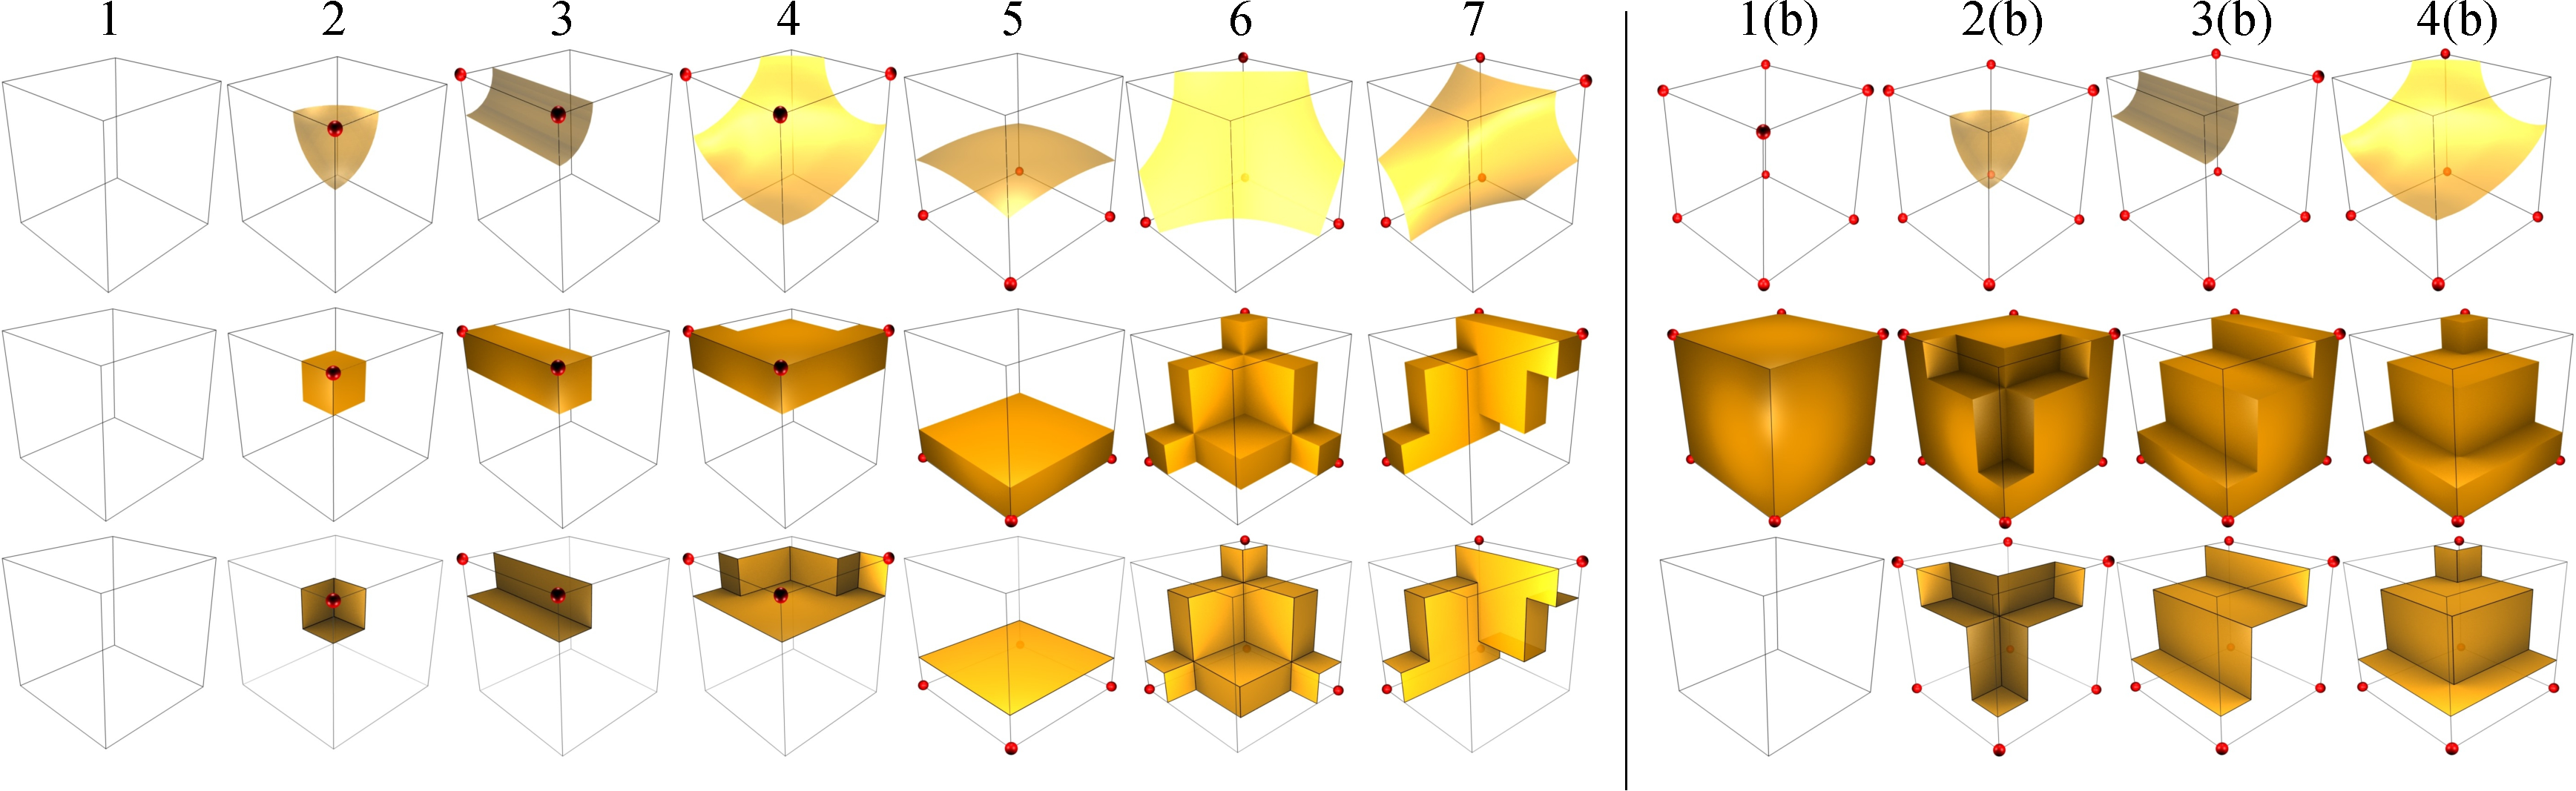
\includegraphics[width=0.95\linewidth,keepaspectratio=true]{chapter3/figures/mi.pdf}
\caption{An illustration of the relation between unambiguous
  isosurfaces of trilinear interpolants and the corresponding digital
  surfaces.  The top row shows all possible configurations of the
  intersection of $t = \alpha$ with a cube $c_j$ for unambiguous
  configurations \cite{lopes:tvcg:2003}.  Each red dot $s_i$ denotes a
  vertex with $e(s_i) < \alpha$. Each image on the top right is the
  complement $\bar{c}_i$ of cases 1 to 4 on the left (cases 5 to 7
  were omitted because the complement is identical to the original
  cube up to symmetry).  The middle row shows the volume reconstructed
  by Majority Interpolation (MI) for configurations 1 to 7 (left) and
  the complements (right) depicted in the top row.  Bottom row shows
  the boundary of the volume reconstructed by the MI algorithm (The
  role of faces that intersect $c_i$ is explained in the proof of
  Theorem~\ref{thm:topological_equivalence_trilinear}).  Notice that
  all surfaces in the top and bottom rows are topological disks. For
  each cube configuration, the boundary of each digital reconstruction
  (bottom row) has the same set of positive/negative connected components as the
  unambiguous configurations (top row).  }
\label{fig:topology_preserving}
\end{center}
\end{figure}

%Digital Topology (DT) is concerned with topological properties of
%\emph{digital images}. Its concepts are largely used in image
%processing literature where it has applications on segmentation,
%thinning, digitization, image repair, among others. In particular,
%the process of 3D digitization of an 3D object remains a challenge
%\cite{siqueira:2007}. Stelldinger et al.  \cite{siqueira:2007}
%present conditions for topological equivalence between 3D objects and
%their digital images. It is mainly based on the concept of
%\emph{r-regular} objects. Loosely speaking, an object is
%\mbox{$r$-regular} if for any point over the surface of the object
%there exist two osculating open balls of radius $r$ such that one is
%completely inside and the other completely outside that object. The
%drawback is that $r$-regular shapes are too restrictive, e. g., is
%does not allow sharp features. Stelldinger and Terzic
%\cite{Stelldinger2008} relaxed this requirement using the concept of
%$r$-halfregular objects, a much wider class of surfaces for which the
%digitization process is guaranteed to preserve the topology of the
%original object.

Let $\mathcal{G}$ be an $n\times n \times n$ cubic regular grid with a
scalar $e(s)$ assigned to each vertex $s$ of $\mathcal{G}$ and
$t:\mathbb{R}^3\rightarrow\mathbb{R}$ be the piecewise trilinear
interpolation function in $\mathcal{G}$, that is, ~~$t(x) = t_i(x)$,
where $t_i$ is the trilinear interpolant in the cubic cell $c_i$
containing $x$.
%
Given a scalar value $\alpha$, the set of points satisfying
$t(x)=\alpha$ is called the \emph{isosurface} $\alpha$ of $t$. In what
follows, $t(x)=\alpha$ will be considered a compact, orientable
2-manifold without boundary.
%The complement of a cubic cell $c_i$ is a cubic cell $\bar{c}_i$ such
%that for each vertex $s_i \in c_i$ and $\bar{s}_i \in \bar{c}_i$ we
%have $e(\bar{s}_i) < \alpha$ if $ e(s_i) > \alpha$ and $e(\bar{s}_i)
%> \alpha$ if $ e(s_i) < \alpha$.
We say that a cubic cell $c_i$ of $\mathcal{G}$ is \emph{unambiguous}
if the following two conditions hold simultaneously:
\begin{enumerate}
\item any two vertices $s_a$ and $s_b$ in $c_i$ for which
  $e(s_a)<\alpha$ and $ e(s_b)<\alpha$ are connected by \emph{negative
  edges}, i. e., a sequence of edges $s_as_1,s_1s_2,\ldots,s_ks_b$ in
  $c_i$ whose vertices satisfy $e(s_i)<\alpha$ for $i=1,\ldots, k$ and
\item any two vertices $s_c$ and $s_d$ in $c_i$ for which
  $e(s_c)>\alpha$ and $e(s_d)>\alpha$ are connected by \emph{positive
  edges}, i. e., a sequence of edges $s_cs_1,s_1s_2,\ldots,s_ls_d$ in
  $c_i$ whose vertices satisfy $e(s_i)>\alpha$ for $i=1,\ldots,l$.
\end{enumerate}
 In other words, a cell is unambiguous if all positive vertices form a
 single connected component via the positive edges and, conversely, all
 negative vertices form a single connected component by negative
 edges~\cite{gelder:tog:1994}.  If either property fails to hold, $c_i$ is called \emph{ambiguous}. The top
 row in Figure~\ref{fig:topology_preserving} shows all possible
 unambiguous cases.

The geometric dual of $\mathcal{G}$ is called the \emph{voxel grid}
associated with $\mathcal{G}$, denoted by $V_{\mathcal{G}}$. More
specifically, each vertex $s$ of $\mathcal{G}$ has a corresponding
voxel $v_s$ in $V_{\mathcal{G}}$, each edge of $\mathcal{G}$
corresponds to a face in $V_{\mathcal{G}}$ (and vice versa), and each
cubic cell in $\mathcal{G}$ corresponds to a vertex in
$V_{\mathcal{G}}$, as illustrated in Figure~\ref{fig:voxelgrid}.  Each
voxel $v_s$ can also be seen as the Voronoi cell associated with $s$.
Scalars defined in the vertices of $\mathcal{G}$ can naturally be
extended to voxels, thus ensuring a single scalar value $e(v_s)$ to
each voxel $v_s$ in $V_{\mathcal{G}}$ defined as $e(s)=e(v_s)$.  As we
shall show, the voxel grid structure plays an
important role when using digital topology to compute topological
invariants of a given isosurface. Before showing that relation,
though, we need a few more definitions.

Denote by $\mathcal{G}^\prime$ the $(2n-1)\times (2n-1) \times (2n-1)$ regular grid
obtained from a refinement of $\mathcal{G}$.
%Scalar values can be defined on the vertices of $\mathcal{G}^\prime$
% using the The piecewise trilinear function $t$ defined above, that
% is, if a vertex $s\in\mathcal{G}^\prime$ is also a vertex of
% $\mathcal{G}$ then the value of $e(s)$ is the same as in
% $\mathcal{G}$ otherwise $s$ lies in a cubic cell $c_i$ of
% $\mathcal{G}$ and $e(s)=t(s)$.
Vertices of $\mathcal{G}^\prime$ can be grouped in four distinct sets,
denoted by $O$, $F$, $E$, $C$. The set $O$ contains the vertices of
$\mathcal{G}^\prime$ that are also vertices of $\mathcal{G}$. The sets
$F$ and $E$ contain the vertices of $\mathcal{G}^\prime$ lying on the
center of faces and edges of the voxel grid $V_{\mathcal{G}}$,
respectively. Finally, $C$ contains all vertices of $V_{\mathcal{G}}$.
Figure~\ref{fig:voxelgrid} illustrates these sets.

Consider now the voxel grid $V_{\mathcal{G^\prime}}$ dual to the
refined grid $\mathcal{G}^\prime$.  Given a scalar value $\alpha$, the
\emph{digital object} $\mathcal{O}_\alpha$ is the subset of voxels $v$
in $V_{\mathcal{G^\prime}}$ such that $v\in\mathcal{O}_\alpha$ if at
least one of the criteria below are satisfied:
\begin{itemize}
\item $v\in O$ and $e(v)\leq\alpha$
\item $v\in F$ and both neighbors of $v$ in $O$ have scalars less than
  (or equal to) $\alpha$
\item $v\in E$ and at least $4$ of the $8$ neighbors of $v$ in $O\cup
  F$ have scalars less than (or equal) $\alpha$
\item $v\in C$ and at least $12$ of the $26$ neighbors of $v$ in
  $O\cup F\cup E$ have scalars less than (or equal) $\alpha$
\end{itemize}
The description above is called Majority Interpolation (MI) 
(Algorithm~\ref{alg:majority-interpolation}), and it allows us to compute
the voxels that belong to a digital object $\mathcal{O}_\alpha$.
%satisfying the above criteria, we use Majority Interpolation (MI), a
%procedure illustrated in Figure~\ref{alg:majority-interpolation}.
%cscheid: I removed the sentence below, because it was in the way of
%the rest of the exposition here. It belongs in the discussion More
%importantly, MI is a simple algorithm, an essential requirement in
%the context of verification.
The middle row of Figure~\ref{fig:topology_preserving} shows all
possible cases for voxels picked by the MI algorithm (notice the
correspondence with the top row of the same figure).

The importance of $\mathcal{O}_\alpha$ is two-fold. First, the
boundary surface of the union of the voxels in $\mathcal{O}_\alpha$,
denoted by $\partial\mathcal{O}_\alpha$ and called a \emph{digital
  surface}, is a $2$-manifold (See the proof by Stelldinger et
al.~\cite{siqueira:2007}). Second, the genus of
$\partial\mathcal{O}_\alpha$ can be computed directly from
$\mathcal{O}_\alpha$ using the algorithm proposed by Chen and Rong
\cite{LiChen:2008} (Algorithm~\ref{alg:compute-invariant}). As the
connected components of $\mathcal{O}_\alpha$ can also be easily
computed and isolated, one can calculate the Euler characteristic of
each connected component of $\mathcal{O}_\alpha$ from the formula
$\chi = 2 - 2g$ and thus $\beta_0$, $\beta_1$, and $\beta_2$.
% cscheid: We should say how that is done here.

The voxel grid $V_{\mathcal{G^\prime}}$ described above allows us to
compute topological invariants for any digital surface
$\partial\mathcal{O}_\alpha$. However, we so far do not have any
result relating $\partial\mathcal{O}_\alpha$ to the isosurface
$t(x)=\alpha$.  The next theorem provides the connection.

\begin{thm}
Let $\mathcal{G}$ be an $n\times n\times n$ rectilinear grid with scalars
associated with each vertex of $\mathcal{G}$ and $t$ be the piecewise trilinear 
function defined on $\mathcal{G}$, such that the isosurface $t(x)=\alpha$ is a
2-manifold without boundary. If no cubic cell of $\mathcal{G}$ is
ambiguous with respect to $t(x)=\alpha$, then $\partial\mathcal{O}_\alpha$
is homeomorphic to the isosurface $t(x)=\alpha$.
\label{thm:topological_equivalence_trilinear}
\end{thm}
{\bf Proof:} Given a cube $c_i \subset \mathcal{G}$ and an isosurface
 $t = \{x \;|\; t(x) = \alpha\}$, let $t_i = t \cap c_i$.  Similarly,
denote
\[\partial \mathcal{O}_i =  cl_{\mathbb{R}^3} \left( (\partial \mathcal{O}_\alpha \cap c_i) - \partial c_i  \right),\]
where $cl_{\mathbb{R}^3}$ denotes the closure operator. We note that
$\partial \mathcal{O}_i$ is a 2-manifold for all $i$
\cite{SPB04,siqueira:2007}.  There are two main parts to the proof
presented here. For each $i$,
\begin{enumerate}
%\vspace{-0.1in}
\item the 2-manifolds $t_i$ and $\partial \mathcal{O}_i$ are homeomorphic; and
%\vspace{-0.1in}
\item both $t_i$ and $\partial \mathcal{O}_i$ cut the same edges and faces of $c_i$.
%\vspace{-0.1in}
\end{enumerate}

Since $t$ is trilinear, no level-set of $t$ can intersect an edge more
than once. Hence, if $c_i$ is not ambiguous, $t_i$ is exactly one of
the cases 1 to 7 in the top row of
Figure~\ref{fig:topology_preserving}~\cite{lopes:tvcg:2003},
either a topological disk or the empty set.  
%
%The digital reconstruction of each unambiguous case is shown in the
%middle row of Figure \ref{fig:topology_preserving}.
%
Each case in the top row of Figure \ref{fig:topology_preserving} is
the unambiguous input for the MI algorithm to produce the voxel
reconstruction shown in the middle row, where the boundaries of each of
these voxel reconstructions are shown in the bottom row.
%
By inspection, we can verify
that the boundary of the digital reconstruction $\partial
\mathcal{O}_i$ (bottom row of Figure \ref{fig:topology_preserving}) is
also a disk for all possible unambiguous cases and complement cases.
Hence, for each $i$, the 2-manifolds $\partial \mathcal{O}_i$ and
$t_i$ are homeomorphic.
%
Then, for each $i$, both $\partial \mathcal{O}_i$ and $t_i$ cut the same
set of edges and faces of $c_i$. Again, we can verify this for all possible $i$
by inspecting the top and bottom rows in Figure \ref{fig:topology_preserving}, respectively.
%
Finally, we apply the Pasting Lemma~\cite{Munkres} across
neighboring surfaces $\partial \mathcal{O}_i$ and $\partial \mathcal{O}_j$ in order to
establish the homeomorphism between $\partial \mathcal{O}_\alpha$
and $t$.
$\Box$
% cscheid: I don't think the Pasting Lemma applies here. The pasting
% lemma is used to create continuous functions in unions of sets by
% combining continuos functions in the subsets and using the natural
% topology. This is not what we need here - since we are trying to
% relate different subsets (the digital reconstructions and the level
% sets of the scalar field) by homeomorphisms. We need something
% stronger. Our other paper has a lemma that might be too strong, but
% is certainly sufficient.

This proof provides a main ingredient for
the verification method in Section~\ref{sec:manufactured}. Crucially, 
we will show how to manufacture a complex solution that
unambiguously crosses every cubic cell of the grid. Since we have
shown the conditions for which the digital surfaces and the level sets
are homeomorphic, any topological invariant will have to be the
same for both surfaces.

\begin{algorithm}
\begin{codebox}
\Procname{$\proc{MajorityInterpolation}(\mathcal{G},\alpha)$}
%\li \Comment Let $S'$ be $S$ with resolution doubled
\li \Comment Let $O$, $F$, $E$ and $C$ be the subset of vertices 
\zi ~~~in $\mathcal{G}^\prime$ as described in
subsection~\ref{sec:digital-topology}. %an old, face, edge and corner point
%\zi  respectively (Definition \ref{dff:majority-interpolation}).
\li \Comment Let $\mathpzc{N}(s, \star)$ be the set of neighbors of
$s\in\mathcal{G}^\prime$ in the \zi ~~~ set $\star$, where $\star =
\{O, F, E, C\}$, with associate scalar \zi ~~~ less than $\alpha$
%\zi of $s \in S'$ inside $p = 0$
\li \For $s \in \mathcal{G}^\prime$
\li     \Do  	\If $s \in O$ \bf or
\li		    $s \in \proc{F}$ and $|\mathpzc{N}(s, O)| = 2$ \bf or
\li			  $s \in E$ and $|\mathpzc{N}(s, O)+\mathpzc{N}(s, F)| 
\geqslant 4$ \bf or
\li		    $s \in \proc{C}$ and $|\mathpzc{N}(s, O)+\mathpzc{N}(s,
F)+\mathpzc{N}(s,E)| \geqslant 12$
\li		\Then Select voxel $v_s$
		\End
	\End
\li \Return $\mathcal{O}_\alpha$
\end{codebox}
\caption{Voxel selection using Majority Interpolation (MI).
}
\label{alg:majority-interpolation}
\end{algorithm}

\begin{algorithm}[ht]
\begin{codebox}
\Procname{$\proc{GenusFromDS}(\partial \mathcal{O}_\alpha)$}
\li \Comment Let $\partial \mathcal{O}_\alpha$ be a 2-manifold without
boundary
\li \Comment Let $|\mathpzc{N}_i|$ be the number of surface points with
\zi ~~~exactly $i$ neighbors.
\li \Comment Let $g$ be the surface genus
\li $g = 1 + (|\mathpzc{N}_5| + 2 |\mathpzc{N}_6| - |\mathpzc{N}_3|) / 8 $
\li \Return $g$
\end{codebox}
\caption{A simple formula for genus computation.}
\label{alg:compute-invariant}
\end{algorithm}

\subsection{Stratified Morse Theory}
\label{sec:smt}
The mathematical developments presented above allow us to compute the
Betti numbers of any isosurface of the piecewise trilinear
interpolant.  However, they require isosurfaces without boundaries.
In this section, we provide a mechanism to compute the Euler
characteristic of any regular isosurface of the piecewise trilinear
interpolant through an analysis based on critical points, which can be
used to verify properties of isosurfaces with boundary components.  We
will use some basic machinery from stratified Morse theory (SMT),
following the presentation of Goresky and MacPherson's
monograph~\cite{Goresky:1988:SMT}.
%We follow the presentation of a separate
%report~\cite{scheidegger:techreport:2010} (submitted as supplementary
%material), which provides a mechanism to compute the Euler
%characteristic of piecewise trilinear isosurfaces using a
%mathematical framework derived from Stratified Morse Theory (SMT)
%\cite{scheidegger:techreport:2010}.

Let $f$ for now be a smooth function with isolated critical points
$p$, where $\nabla f(p) = 0$.  From classical Morse theory, the
topology of two isosurfaces $f(x)=\alpha$ and $f(x)=\alpha+\epsilon$
differs only if the interval $[\alpha, \alpha + \epsilon]$ contains a
critical value ($f(p)$ is a critical value iff $p$ is a critical
point). Moreover, if $\varepsilon_p$ is a small neighborhood around
$p$ and $L^-(p)$ and $L^+(p)$ are the subset of points on the boundary
of $\varepsilon_p$ satisfying $f(x)<f(p)$ and $f(x)>f(p)$
respectively, then the topological change from the isosurface
$f(x)=f(p)-\epsilon$ to $f(x)=f(p)+\epsilon$ is characterized by
removing $L^-(p)$ and attaching $L^+(p)$. Thus, changes in the Euler
characteristic, denoted by $\Delta\chi(p)$, are given by:
\begin{equation}
\Delta\chi(p) = \chi(L^+(p)) - \chi(L^-(p)).
\label{eq:deltachi}
\end{equation}
% \noindent where $\chi(L^-(p))$ and $\chi(L^+(p))$ are the Euler characteristic of $L^-(p)$ and $L^+(p)$,
% respectively. 
\noindent For a smooth function $f$, the number of negative eigenvalues of the
Hessian matrix determines the index of a critical point $p$, and the
four cases give the following values for $\chi(L^-(p))$
and $\chi(L^+(p))$:
%In the smooth scenario, $\chi(L^-(p))$ and $\chi(L^+(p))$
%can be inferred from the number of negative eigenvalues of the Hessian
%matrix of $f$ in $p$, and we have four distinct cases:
\begin{center}
\begin{tabular}{c|c|c|c|c}
& min & saddle-1 & saddle-2 & max \\
\hline
$\chi(L^-(p))$ & 0 & 2 & 0 & 2 \\ 
$\chi(L^+(p))$ & 2 & 0 & 2 & 0
\end{tabular}
\end{center}
The above formulation is straightforward but unfortunately cannot be directly applied to
functions appearing in either piecewise trilinear interpolations or
isosurfaces with boundary, both of which
appear in some of the isosurfacing algorithms with guaranteed
topology. Trilinear interpolants are not smooth across the faces
of grid cells, so the gradient is not well-defined there. Identifying the
critical points using smooth Morse theory is then
problematic. Although arguments based on smooth Morse
theory have appeared in the
literature~\cite{Weber:2002:ESF}, there are complications. For
example, the scalar field in a node
of the regular grid might not have \emph{any} partial
derivatives. Although one can still argue about the
intuitive concepts of minima and maxima around a non-differentiable point,
configurations such as saddles are more problematic, since their
topological behavior is different depending on whether they are on the
boundary of the domain. It is 
important, then, to have a mathematical tool which makes predictions
regardless of the types of configurations, and SMT is one such theory.

\begin{figure}
\includegraphics[width=\linewidth]{chapter3/figures/stratification.png}
\caption{\label{fig:stratification}An illustration of a
  piecewise-smooth immersed 2-manifold. The colormap illustrates the
  value of each point of the scalar field. Notice that although the manifold
  itself is not everywhere differentiable, each stratum is itself an open
  manifold that is differentiable.}
\end{figure}

Intuitively, a \emph{stratification} is a partition of a
piecewise-smooth manifold such that each subset, called a
\emph{stratum}, is either a set of discrete points or has a smooth
structure.  In a regular grid with cubic cells, the stratification we
propose will be formed by four sets (the strata), each one a (possibly
disconnected) manifold.  The \emph{vertex set} contains all vertices
of the grid. The \emph{edge set} contains all edge interiors, the
\emph{face set} contains all face interiors, and the \emph{cell set}
contains all cube interiors. We illustrate the concept for the 2D case
in Figure~\ref{fig:stratification}.  The important property of the
strata is that the level sets of $f$ restricted to each stratum are
smooth (or lack any differential structure, as in the vertex-set). In
SMT, one applies standard Morse theory on each stratum, and then
combines the partial results appropriately.

The set of points with zero gradient (computed on each stratum), which
SMT assumes to be isolated, are called the \emph{critical points} of
the stratified Morse function. In addition, every point in the vertex
set is considered critical as well. One major difference between SMT
and the smooth theory is that some critical points do not actually
change the topology of the level sets. This is why considering all
grid vertices as critical does not introduce any practical problems:
most grid vertices of typical scalar fields will be \emph{virtual
  critical points}, {\em i.e.}, points which do not change the Euler
characteristic of the surface. Carr and Snoeyink use a
related concept (which they call ``potential critical points'') in
their state-machine description of the topology of
interpolants~\cite{CS08}.

Let $\mathcal{M}$ be the stratified grid described above.  It can be
shown that if $p$ is a point in a $d$-dimensional stratum of
$\mathcal{M}$, it is always possible to find a $(3-d)$-dimensional
submanifold of $\mathcal{M}$ (which might straddle many strata) that
meets transversely the stratum containing $p$, and whose intersection
consists of only $p$ (one way to think of this $(3-d)$-manifold is as a ``topological orthogonal
complement'').  In this context, we can define a small neighborhood
$T_\varepsilon(p)$ in the strata containing $p$ and the \emph{lower
  tangential} link $T_L^-(p)$ as the set of points in the boundary of
$T_\varepsilon(p)$ with scalar values less than that in $p$.
\begin{wrapfigure}{r}{2.5cm}
\vspace{-0.2cm}
\includegraphics[width=2.0cm,keepaspectratio=true]{chapter3/figures/ilustration.png}
\end{wrapfigure}
Similarly we can define the \emph{upper tangential} link $T_L^+(p)$ as
the set of points in the boundary of $T_\varepsilon(p)$ with scalar
value higher than that at $p$.  \emph{Lower normal} $N_L^-(p)$ and
\emph{upper normal} $N_L^+(p)$ links are analogous notions, but the
lower and upper links are taken to be subsets of $N_\varepsilon(p)$,
itself a subset of the $(3-d)$-dimensional submanifold transverse to
the stratum of $p$ going through $p$.  The definitions above are needed
in order to define the \emph{lower stratified link} and \emph{upper
  stratified link}, as follows: given $T_\varepsilon(p),\,
T_L^-(p),\,N_\varepsilon(p)$ and $N_L^-(p)$, the \emph{lower
  stratified Morse link} (and similarly for upper stratified link) is
given by
\begin{equation}
L^-(p) = (T_\varepsilon(p) \times N_L^-(p)) \cup (N_\varepsilon(p)
\times T_L^-(p)) \label{eq:lowerstratifiedlink}.
\end{equation}
These definitions allow us to classify critical points even in the non-smooth scenario.
They let us compute topological changes with
the same methodology used in the smooth case. In other words, when a
scalar value $\alpha$ crosses a critical value $\alpha_p$ in a
critical point $p$, the topological change in the isosurface is
characterized by removing $L^-(p)$ and attaching $L^+(p)$, affecting
the Euler characteristic as defined in Equation~\ref{eq:deltachi}.%\cite{?}.

The remaining problem is how to determine $\chi(L^-(p))$ and
$\chi(L^+(p))$. 
Recalling that $\chi(A \cup B) = \chi(A) + \chi(B) - \chi(A \cap B)$,
$\chi(A\times B)=\chi(A)\chi(B)$, and $\chi(T_\varepsilon)=\chi(N_\varepsilon)=1$ (we are omitting 
the point $p$) we have:
\begin{equation}
\begin{array}{l}
\chi(L^-) = \chi(T_\varepsilon \times N_L^- \cup N_\varepsilon \times T_L^-) \\
    \qquad  = \chi(N_L^-) + \chi(T_L^-) - \chi(T_\varepsilon \times N_L^- \cap N_\varepsilon \times T_L^-)
\end{array}
\end{equation}
Now, we can define $T_\varepsilon = T_L^- \cup T_r,\, T_L^- \cap T_r =
\emptyset$ and similarly for $N_\varepsilon$ and $N_L^-$.  Then,
expand the partitions and products, and distribute the intersections
around the unions, noticing all but one of intersections will be
empty:
\begin{eqnarray*}
T_\varepsilon \times N_L^- \cap N_\varepsilon \times T_L^- \hspace{-8.0px} &=& \hspace{-8.0px} ((T_r \cup T_L^-) \times N_L^-) \cap ((N_r \cup N_L^-) \times T_L^-) \\
\hspace{-8.0px} &=& \hspace{-8.0px} ((T_r \times N_L^-) \cup (T_L^- \times N_L^-)) \cap \\
\hspace{-8.0px} && \hspace{-8.0px}((N_r \times T_L^-) \cup (N_L^- \times T_L^-)) \\
\hspace{-8.0px} &=& \hspace{-8.0px}N_L^- \times T_L^-
\end{eqnarray*}
Therefore:
\begin{eqnarray*}
\chi(T_\varepsilon \times N_L^- \cap N_\varepsilon \times T_L^-) &=& \chi(N_L^- \times T_L^-) \\
&=& \chi(N_L^-)\chi(T_L^-)
\end{eqnarray*}
which gives the final result
\begin{equation}
\chi(L^-) = \chi(N_L^-)+\chi(T_L^-)-\chi(N_L^-)\chi(T_L^-) \label{eq:lowerchi}.
\end{equation}

The same result is valid for $\chi(L^+)$, if we replace the 
superscript `$-$' by `$+$' in Equation~\ref{eq:lowerchi}. If $T_L^-$ or
$T_L^+$ are one-dimensional, then we are done. If not, then we can
recursively apply the same equation to $T_L^-$ and $T_L^+$ and look at
progressively lower-dimensional strata until we reach
$T_\varepsilon(p)$ and $N_\varepsilon(p)$ given by $1$-disks. The
lower and upper links for these \mbox{$1$-disks} will always be
discrete spaces with zero, one, or two points, for which $\chi$ is
simply the cardinality of the set.

In some cases, the Euler characteristic of the lower and upper link
might be equal. Then, $\chi(L^-(p)) = \chi(L^+(p))$, and
$\Delta\chi(p) = 0$. These cases correspond to the virtual critical
points mentioned above.
%, that is, critical points which do not change
%the Euler characteristic of the surface.
%
Critical points in the interior of cubic cells are handled by the
smooth theory, since in that case the normal Morse data is
0-dimensional. This implies that the link will be an empty set with
Euler characteristic zero. So, by Equation~\ref{eq:lowerchi},
$\chi(L^-) = \chi(T_L^-)$. Because the restriction of the scalar field
to a grid edge is a linear function, no critical point can appear
there. As a result, the new cases are critical points occurring at
vertices or in the interior of faces of the grid.  For a critical
point $p$ in a vertex, stratification can be carried out recursively,
using the edges of the cubes meeting in $p$ as tangential and normal
submanifolds. Denoting by $n_{l1},n_{l2},n_{l3}$ the number of
vertices adjacent to $p$ with scalar value less than that of $p$ in
each Cartesian coordinate direction, Equation~(\ref{eq:lowerchi})
gives:
\begin{equation}
\chi(L^-(p)) = n_{l1}+n_{l2}+n_{l3} - n_{l1}(n_{l2}+n_{l3})
\end{equation}
$\chi(L^+(p))$ can be computed similarly, but considering the number of neighbors of $p$ in each Cartesian 
direction with scalars higher than that of $p$.

If $p$ is a critical point lying in a face $r$ of a cube, we consider
the face itself as the tangential submanifold and the line segment
$r^\perp$ orthogonal to $r$ through $p$ the normal submanifold.
Recursively, the tangential submanifold can be further stratified in
two $1$-disks (tangential and normal).  Denote by $n_l$ the number of
ends of $r^\perp$ with scalar value less than that of $p$. Also,
recalling that the critical point lying in the face $r$ is necessarily
a saddle, thus having two face corners with scalar values less and two
higher than that of $p$, Equation~(\ref{eq:lowerchi}) gives:
\begin{equation}
\chi(L^-(p)) = n_l+2 - 2\,n_l
\end{equation}
Analogously, we can compute $\chi(L^+(p)) = n_u+2 - 2\,n_u$ where
$n_u$ is the number of ends of $r^\perp$ with scalar value higher than
that of $p$.

A similar analysis can be be carried out for every type of critical
point, regardless of whether the point belongs to the interior of a
grid cell (and so would yield equally well to a smooth Morse theory
analysis), an interior face, a boundary face, or a vertex of any
type. The Euler characteristic $\chi_\alpha$ of any isosurface with
isovalue $\alpha$ is simply given as:
\begin{equation}
\chi_\alpha = \sum_{p_i\in C_\alpha} \Delta\chi(p_i)
\label{ref:chis}
\end{equation}
where $C_\alpha$ is the set of critical points with critical values less than $\alpha$.

It is worth mentioning once again that, to the best of our knowledge,
no other work has presented a scheme which provides such a simple
mechanism for computing the Euler characteristic of level sets of
piecewise-smooth trilinear functions. Compare, for example, the case
analyses and state machines performed separately by
Nielson~\cite{Nielson03onmarching}, by Carr and Snoeyink~\cite{CS08},
and by Carr and Max~\cite{CM10}. In contrast, we can recover an
(admittedly weaker) topological invariant by a much simpler
argument. In addition, this argument already generalizes (trivially
because of the stratification argument) to arbitrary dimensions,
unlike the other arguments in the literature.


\section{Manufactured Solution Pipeline}
\label{sec:manufactured}

We now put the pieces together and build a pipeline for topology 
verification using the results presented in Section~\ref{sec:math-foundations}. 
In the following sections, the procedure called $\proc{Isosurfacing}$ refers to the
isosurface extraction technique under verification.
$\proc{InvariantFromMesh}$ computes topological invariants of a simplicial
complex. 
%Section \ref{sec:discussion} compares the verification pipelines using
%Digital Topology and Stratified Morse Theory.


\subsection{Consistency}
\label{sec:consistency-verification}

As previously mentioned, MC-like algorithms which use
disambiguation techniques are expected to generate PL manifold isosurfaces no matter how complex 
the function sampled in the vertices of the regular grid. 
In order to stress the consistency test, we generate a random scalar field with values in the
interval $[-1,1]$ and extract the isosurface with isovalue $\alpha=0$
(which is all but guaranteed not to be a critical value) using a
given isosurfacing technique, subjecting the 
resulting triangle mesh to the consistency verification. This process
is repeated a large number of times, and  
%
if the implementation fails to
produce \mbox{PL manifolds} for all cases, then the counterexample
provides a documented starting point for debugging. If it passes the
tests, we consider the implementation verified.
% (in the sense of analyzed predicted behavior) for all test cases to which
% it has been applied, increasing our confidence in the stated properties

\begin{algorithm}
\begin{codebox}
\Procname{$\proc{MMS-SMT}(\mathcal{G})$}
\li \Comment Let the input $\mathcal{G}$ be $n \times n \times n$ rectilinear grid
\li \For $i \gets 1$ \To $\#$tests
\li     \Do $\mathcal{G} \gets$ randomly sampled $n \times n \times n$ grid \label{alg:mms:sampling}
\li         $\id{CPs} \gets \proc{ComputeCriticalPoints}(\mathcal{G})$
\li         \If $p \in CPs$ is degenerate \kw{or}
\li		$p$ is an internal saddle close to edges or faces
\li         	\Then $\proc{GoTo}$ \ref{alg:mms:sampling} \label{alg:mms:goto-smt}
\li         \Else $K \gets \proc{Isosurfacing}(\mathcal{G})$
\li         	  $(\chi^v)_i \gets \proc{InvariantFromCPs}(\mathcal{G})$
\li         	  $(\chi^k)_i \gets \proc{InvariantFromMesh}(K)$
	    \End
\li Compare $(\chi^v)_i$ and $(\chi^k)_i$
      \End
\end{codebox}
\caption{Overview of the method of manufactured solutions (MMS) using
stratified Morse theory. \proc{InvariantFromCPs} is computed using Equation
\ref{ref:chis}. The method either fails to match the expected topology, in
which case $\mathcal{G}$ is provided as a counterexample, or
succeeds otherwise.}
\label{alg:manufactured-solutions-smt}
\end{algorithm}

\subsection{Verification using Stratified Morse Theory}
\label{subsec:smt-verify}

We can use the formulation described in Section~\ref{sec:smt} to
verify isosurfacing programs which promise to match the
topology of the trilinear interpolant.
The SMT-based verification procedure is summarized in
Algorithm~\ref{alg:manufactured-solutions-smt}. The algorithm 
has four main steps. A random scalar field with node values in the
interval $[-1,1]$ is initially created. Representing the trilinear
interpolation in a grid cell by $f(x,y,z) = axyz + bxy + cxz + dyz + ex + fy + gz + h$,
the internal critical points are given by:
\[\begin{array}{ccc}
t_x = (d \Delta_x \pm \sqrt{\Delta_x \Delta_y \Delta_z})/({a \Delta_x})\\
t_y = (c \Delta_y \pm \sqrt{\Delta_x \Delta_y \Delta_z})/({a \Delta_y})\\
t_z = (b \Delta_z \pm \sqrt{\Delta_x \Delta_y \Delta_z})/({a \Delta_z}),
\end{array}\]
%% \begin{eqnarray*}
%% t_x &=&  \\
%% t_y &=&  \\
%% t_z &=&  
%% \end{eqnarray*}
\noindent where $\Delta_x = bc-ae$, $\Delta_y = bd-af$, and $\Delta_z
= cd-ag$~\cite{Pascucci03}.  Critical points on faces of the cubes are found by setting
$x,y$ or $z$ to either 0 or 1, and solving
the quadratic equation.  
If the solutions lie outside the unit cube $[0, 1]^3$, they are not
considered critical points, since they lie outside the domain of the cell. The scalar field
is regenerated if any degenerate critical point is detected (these
can happen if either the random values in a cubic cell have, by chance, the same value or when 
$\Delta_x$, $\Delta_y$ or $\Delta_z$ are zero). In order
to avoid numerical instabilities, we also regenerate the scalar field
locally if any internal critical point lies too close to the border of
the domain (that is, to an edge or to a face of the cube).

The third step computes the Euler characteristic of a set of
isosurfaces with random isovalues in the interval $[-1, 1]$ using the
theory previously described, jointly with Equation~\ref{ref:chis}.  In
the final step, the triangle mesh $M$ approximating the isosurfaces is
extracted using the algorithm under verification, and $\chi(M) = V(M)
- E(M) + F(M)$, where $V(M),E(M)$, and $F(M)$ are the number of
vertices, edges, and triangles. If the Euler characteristic computed
from the mesh does not match the one calculated via
Equation~\ref{ref:chis}, the verification fails. We carry out the
process a number of times, and implementations that pass the tests are
less likely to contain bugs.

\subsection{Verification using Digital Topology}
\label{subsec:ds-verify}

\begin{figure}
\centering
\includegraphics[width=1.0\linewidth,keepaspectratio=true]
{chapter3/figures/trilinear-field.pdf}
\caption{Our manufactured solution is given by $t(x) = \alpha$. $\mathcal{G}$ is
depicted in solid lines while $\tilde{\mathcal{G}}$ is shown in dashed lines.
$\tilde{\mathcal{G}}$ is a uniform subdivision of $\mathcal{G}$. The trilinear
surfaces $t_i$ are defined for each cube
$c_i \in \mathcal{G}$ and resampled in $c'_j \in \tilde{\mathcal{G}}$.
The cubes in the center of $\mathcal{G}$ have four maxima each
(left) and thus induce complicated topology. The final
isosurface may have several tunnels and/or connected
components even for coarse $\mathcal{G}$ (right). }
\label{fig:trilinear-field}
\end{figure}


Algorithm~\ref{alg:manufactured-solutions-digital-surfaces} shows the
verification pipeline using the MI algorithm, and
Figure~\ref{fig:trilinear-field} depicts the refinement process. Once
again a random scalar field, with potentially many ambiguous cubes, is
initially generated in the vertices of a grid $\mathcal{G}$.  The
algorithm illustrated in
Algorithm~\ref{alg:manufactured-solutions-digital-surfaces} is applied to
refine $\mathcal{G}$ so as to generate a new grid
$\tilde{\mathcal{G}}$ which does not have ambiguous cells. If the
maximum number of refinement is reached and ambiguous cells still
remain, then the process is restarted from scratch.  Notice that cube
subdivision does not need to be uniform.  For instance, each cube may
be refined using a randomly placed new node point or using $t_i$'s
critical points, and the result of the verification process still
holds.  This is because Theorem
$\ref{thm:topological_equivalence_trilinear}$ only requires $c_i$ to
be unambiguous.
%This shows us that the reliability of this verification process depends 
%only on key concepts with other steps performed in
%possibly many different ways. 
For simplicity, in this work we refine $\mathcal{G}$ uniformly
doubling the grid resolution in each dimension.

Scalars are assigned to the new vertices of $\tilde{\mathcal{G}}$ (the ones not in $\mathcal{G}$) by trilinearly 
interpolating
from scalars in $\mathcal{G}$, thus ensuring that $\mathcal{G}$ and  $\tilde{\mathcal{G}}$ have
exactly the same scalar field~\cite{Nielson03onmarching}.
As all cubic cells in $\tilde{\mathcal{G}}$ are unambiguous, Theorem \ref{thm:topological_equivalence_trilinear} guarantees 
the topology of the digital surface $\partial\mathcal{O}_\alpha$
obtained from $\tilde{\mathcal{G}}$ is equivalent to 
that of $t(x)=\alpha$. Algorithm \proc{InvariantFromDS} computes
topological invariants of
$\partial\mathcal{O}_\alpha$ using the scheme discussed in
Section~\ref{sec:digital-topology}. In this context, \proc{InvariantFromDS} is
the algorithm illustrated in Algorithm~\ref{alg:compute-invariant}.
Surfaces with boundary are avoided by assigning the scalar value $1$ to every vertex in the
boundary of $\mathcal{G}$.
%$\proc{RefineAndResample}$ generates $S'$, a refined version of
%$S$ that contains no ambiguous cases. Theorem \ref{thm:topological_equivalence_trilinear} guarantees that if no ambiguous cells exist the topology of the digitized surface $\partial V$ is the same as $p = 0$. 
%Notice that the subdivison part of \proc{RefineAndResample} can be done using many different schemes. 
%For instance, each cube may be refined in a non-uniform way, using a random pivot or using $p_i$'s critical points, 
%and the result of the verification process is still reliable. 
%This is because Theorem $\ref{thm:topological_equivalence_trilinear}$ only requires that each $C$ to be unambiguous. 
%In fact, $C$ doesn't even have to be a cube. This shows us that the reliability of this verification 
%process depends only on key concepts with other steps beign done in arbitrarily ways. 
%Although not stricly necessary, the refinement applied to $\mathcal{G}$ to generate $\tilde{\mathcal{G}}$ is uniform. 
%In fact, we set maximum number of refinements to be applied, if the upper bound is reached and ambiguous cells
%are still present in the grid, we restart the process from scratch, generating a new random field in $\mathcal{G}$
%and triggering then the refinement process.
%It is important to point out that If no $S'$ can be found for a particular $S$, the process is restarted. Although this reduces the range
%of $p$ defined in $C_i$, in our tests we hit all 256 possible combinations of signs for
%$C_i$ (Figure \ref{fig:trilinear-field} shows an instance of $p = 0$). $\proc{InvariantFromDS}$ uses the algorithm described in \ref{sec:digital-topology} for computing digital surface invariants.
%Among the advantages of this framework is the simplicity and ability of compute
%topological invariants, namely, the Euler Characteristics $\chi$,
%$\beta_0$, $\beta_1$ and $\beta_2$. On the other hand, the zero level-set must
%be a closed 2-manifold.




% \begin{figure}
% \begin{codebox}
% \Procname{$\proc{MajorityInterpolation}(S)$}
% \li \Comment Let $S'$ be $S$ with resolution doubled
% \li \Comment Let $O$, $F$, $E$ and $C$ be an old, face, edge and corner point
% \zi  respectively (Definition \ref{dff:majority-interpolation}).
% \li \Comment Let $\mathpzc{N}(s, t)$ be the set of $t-$neighbors, $t \in \{O,
% F, E, C\}$ 
% \zi of $s \in S'$ inside $p = 0$
% \li \For $s \in S'$
% \li     \Do  	\If $s = O$ \bf or
% \li		    $s = \proc{F}$ and $|\mathpzc{N}(s, O)| = 2$ \bf or
% \li			  $s = E$ and $|\mathpzc{N}(s, O)+\mathpzc{N}(s, F)| 
% \geqslant 4$ \bf or
% \li		    $s = \proc{C}$ and $|\mathpzc{N}(s, O)+\mathpzc{N}(s,
% F)+\mathpzc{N}(s,E)| \geqslant 12$
% \li		\Then Select voxel $\mathpzc{V}_{S'}(s)$
% 		\End
% 	\End
% \li \Return $S'$
% \end{codebox}
% \caption{Voxel selection.}
% \label{alg:majority-interpolation}
% \end{figure}

\begin{algorithm}
\begin{codebox}
\Procname{$\proc{MMS-DS}(\mathcal{G})$}
\li \Comment Let the input $\mathcal{G}$ be a $n \times n \times n$ rectilinear grid
\li \For $i \gets 1$ \To $\#$tests
\li     \Do  $\mathcal{G} \gets$ randomly sampled $n \times n \times n$ grid \label{alg:mms:sampling2}
\li         $\tilde{\mathcal{G}} \gets \proc{RefineAndResample}(\mathcal{G})$
\li         \If $\tilde{\mathcal{G}}$ has ambiguous cubes
\li         	\Then $\proc{GoTo}$ \ref{alg:mms:sampling2} \label{alg:mms:goto-dt}
			\End
\li         $\mathcal{O} \gets
\proc{MajorityInterpolation}(\tilde{\mathcal{G}})$
\li 		  $K \gets \proc{Isosurfacing}(\mathcal{G})$
\li         	  $(\beta_0^v, \beta_1^v,\beta_2^v)_i \gets
\proc{InvariantFromDS}(\partial {\mathcal{O}})$
\li         	  $(\beta_0^k, \beta_1^k,\beta_2^k)_i \gets
\proc{InvariantFromMesh}(K)$
\li Compare $(\beta_0^v, \beta_1^v,\beta_2^v)_i$ and $(\beta_0^k, \beta_1^k,\beta_2^k)_i$
	    \End
      \End
\end{codebox}
\caption{Overview of the method of manufactured solutions (MMS) using digital
topology. The method either fails to match the expected topology, in
which case $\mathcal{G}$  is provided as a counterexample, or
succeeds otherwise.}
\label{alg:manufactured-solutions-digital-surfaces}
\end{algorithm}



\section{Experimental Results}
\label{sec:results}

In this section, we present the results of applying our topology verification
methodology to a number of different isosurfacing techniques, 
three of them with topological guarantees with respect to trilinear interpolant.
Specifically, the techniques are:

\vtk\ \cite{vtk} is the Visualization Toolkit (VTK) implementation of the
Marching Cubes algorithm with the
implicit disambiguation scheme proposed by Montani et al.
\cite{Montani:1994:MLT}. Essentially, it separates positive vertices when a
face saddle appears and assumes no tunnels exist inside a cube. The
proposed scheme is topologically consistent, but it does not reproduce the
topology of the trilinear interpolant. 

Marching Cubes with Edge Transformations or \macet\ \cite{Dietrich:TVCG:2008} is
a Marching Cubes-based technique designed to generate triangle 
meshes with good quality. 
%The authors show that approximately parallel intersections
%between an isosurface and a grid cube are responsible for bad triangle quality.
Quality is reached by displacing active edges of the grid (edges intersected by the
isosurface), both in normal and tangential direction toward avoiding ``sliver'' intersections. 
%The results presented shows substancial improvement on mesh quality. 
Macet does not reproduce the topology of the trilinear interpolant.

\afront~\cite{Schreiner06} is an advancing-front method for isosurface
extraction, remeshing, and triangulation of point sets. It works by advancing
triangles over an implicit surface. A sizing function that takes curvature into account
is used to adapt the triangle mesh to features of the
surface. \afront\ uses cubic spline reconstruction kernels to
construct the scalar field from a regular grid.
%is derived from a Afront's main feature is a
%special scheme for adapting triangle size according to surface curvature.
The algorithm produces high-quality triangle meshes with bounded
Hausdorff error. As occurred with the VTK and Macet implementations, Afront produces consistent
surfaces but, as expected, the results do not match the trilinear
interpolant.

\matlab$^\circledR$ \cite{matlab10} is a high-level language for building codes that requires intensive
numerical computation. It has a number of features and among them an isosurface extraction routine for volume data
visualization. Unfortunately, \matlab\ documentation does not offer information
on the particularities of the implemented isosurface extraction technique (e.g., Marching Cubes, Delaunay-based, etc; consistent or correct).

\snapmc\ \cite{Raman:2008:QIM} is a Marching Cubes variant which produces high-quality 
triangle meshes from regular grids. The central idea is to extend the 
original lookup table to account for cases where the isosurface passes exactly through the 
grid nodes. Specifically, a user-controlled parameter dictates maximum distance 
for ``snapping'' the isosurface into the grid node. 
The authors report an improvement in the minimum triangle angle when compared to previous techniques.


\mclewiner\ was introduced by Chernyaev
\cite{Chernyaev95marchingcubes} to solve ambiguities in the original MC. It
extends Marching Cubes table from 15 to 33 cases to account for ambiguous cases
and to reproduce the topology of the trilinear interpolant inside each cube. The
original table was later modified to remove two redundant cases which leads to 31
unique configurations. Chernyaev's MC solves face ambiguity using Nielsen and
Hamann's \cite{Nielson1991} asymptotic decider and internal ambiguity
by evaluating the bilinear function over a plane parallel to a face. Additional
points may be inserted to reproduce some configuration requiring subvoxel
accuracy.  We use Lewiner et al.'s implementation \cite{Lewiner:2003} of
Chernyaev's algorithm.

\deliso\ \cite{Dey07} is a Delaunay-based approach for isosurface extraction. 
It uses the intersection of the 3D Voronoi diagram and the desired surface to 
define a restricted Delaunay triangulation. Moreover, it
builds the restricted Delaunay triangulation without having to
compute the whole 3D Voronoi structure. \deliso\ has theoretical guarantees of
homeomorphism and mesh quality.

\mcsimpleflow\ is a proof-of-concept implementation of the algorithm
described in Scheidegger et al.
\cite{scheidegger:techreport:2010}. It works by successive cube
subdivision until it has a \emph{simple edge flow}. A cube has a
simple edge flow if it has only one \emph{minima} and one
\emph{maxima}. A vertex $s \in c_i$ is a minimum if all vertices $s_j
\in c_i$ connected to it has $t(s_j) > t(s_i)$. Similarly, a vertex is
a maximum if $t(s_j) < t(s_i)$ for every neighbor vertex $j$.  This
property guarantees that the Marching Cubes method will generate a
triangle mesh homeomorphic to the isosurface. After subdivision, the
surfaces must be attached back together. The final mesh is
topologically correct with respect to the trilinear interpolant.

We believe that the implementation of any of these algorithms in full
detail is non-trivial. The results reported in the following section
support this statement. They show that coding isosurfacing algorithms
is complex and error-prone, and they reinforce the need for robust
verification mechanisms.
%are intended only to stress the complexity involved in coding
%isosurfacing techniques and to show that our framework may help
%developers to find and gain confidence in the implementation.
In what follows, we say that a \emph{mismatch} occurs when invariants
computed from a verification procedure disagree with the invariants
computed from the isosurfacing technique.  A mismatch does not
necessarily mean an implementation is incorrect, as we shall see later
in this section.  After discussions with the developers, however, we
did find that there were bugs in some of the implementations.

\subsection{Topology consistency}
\label{sec:consistency}

All implementations were subject to the consistency test 
(Section \ref{sec:consistency-verification}), resulting in the outputs
reported in the first column of 
Table~\ref{tbl:verification-ds-stm}. We observed mismatches for
\deliso, \snapmc\ (with non-zero snap value), and \matlab\ 
implementations. Now, we detail these results.

% Although the focus of the paper is on topology correctness, we present the
% results for topology consistency for completeness.
\subsubsection{\deliso}
\label{sec:consistency:deliso}
We analyzed $50$ cases where \deliso's output mismatched the ground
truth produced by MMS, and we found that: 1) $28$ cases had incorrect
hole(s) in the mesh, 2) $15$ cases had missing triangle(s), and 3) $7$
cases had duplicated vertices.  These cases are illustrated in Figure
\ref{fig:pproblem-deliso}.  The first problem is possibly due to the
non-smooth nature of the piecewise trilinear interpolant, since in all
$28$ cases the holes appeared in the faces of the cubic grid. It is
important to recall that \deliso\ is designed to reproduce the
topology of the trilinear interpolant inside each grid cube, but the
underlying algorithm requires the isosurface to be $C^2$ continuous
everywhere, which does not hold for the piecewise trilinear
isosurface.
%are only guranteed to be $C^0$. 
In practice, real world datasets such as medical images may induce
``smoother'' piecewise trilinear fields when compared to the extreme
stressing from the random field, which should reduce the incidence of
such cases. Missing triangles, however, occurred in the interior of
cubic cells where the trilinear surface is smooth.
%This might occur due to 
Those problems deserve a deeper analysis, as one cannot say beforehand
if the mismatches are caused by problems in the code or numerical
instability
%We attribute that to numerical instabilities associated with the
%isosurfacing process.
associated with the initial sampling, ray-surface intersection, and the
3D Delaunay triangulation construction.
%may compromises the construction of the restricted delaunay. 

\subsubsection{\snapmc}

Table \ref{tbl:verification-ds-stm} shows that \snapmc\ with non-zero snap value
causes the mesh to be topologically inconsistent (Figure 
\ref{fig:inconsistencies:snapmc}) in more the 50\% of the performed tests. 
The reason for this behavior is in the heart of the technique: the snapping process 
causes geometrically close vertices to be merged together 
which may eliminate connected components, or loops, join connected
components or even create non-manifold surfaces. This is why there was an increase
in the number of mismatches when compared with \snapmc\ with zero snap value.
Since non-manifold meshes are not desirable in many applications, the authors 
suggest a post-processing for fixing these topological issues, although no implementation
or algorithm for this post-processing is provided.

\subsubsection{\matlab}

\matlab\ documentation does not specify the properties of the
implemented isosurface extraction technique. Consequently, it becomes
hard to justify the results for the high number of mismatches we see
in Table \ref{tbl:verification-ds-stm}.  For instance, Figure
\ref{fig:inconsistencies:matlab} shows an example of a non-manifold
mesh extracted using \matlab. In that figure, the two highlighted
edges have more than two faces connected to them and the faces between
these edges are coplanar.  Since we do not have enough information to
explain this behavior, this might be the actual expected behavior or
an unexpected side effect. An advantage of our tests is the record of
the observed behavior of mesh topologies generated by \matlab.

\subsubsection{\macet}

In our first tests, \macet\ failed in all consistency tests for a $5 \times 5 \times 5$ grid. 
%resolution because the way it traverse the volume for building the triangulation. 
An inspection in the code revealed that the layer of cells in the boundary of the grid
has not been traversed. Once that bug was fixed, \macet\ started to produce
PL manifold
meshes and was successful in the consistency test, as shown in Table~\ref{tbl:verification-ds-stm}.

\subsection{Topology correctness}
\label{sec:correctness}


The verification tests described in Section \ref{subsec:smt-verify}
and \ref{subsec:ds-verify} were applied to all algorithms, although
only \mclewiner, \deliso, and \mcsimpleflow\ were expected to generate
meshes with the same topology of the trilinear interpolant. Our tests
consisted of one thousand random fields generated in a rectilinear $5
\times 5 \times 5$ grid $\mathcal{G}$.  The verification test using
Digital Surfaces demanded a compact, orientable, 2-manifold without
boundary, so we set scalars equal $1$ for grid vertices in the
boundary of the grid.  As stratified Morse theory supports surfaces
with boundary, no special treatment was employed in the boundary of
$\mathcal{G}$. We decided to run these tests using all algorithms for
completeness and also for testing the tightness of the theory, which
says that if the algorithms do not preserve the topology of the
trilinear interpolant, a mismatch should occur.  Interestingly, with
this test, we were able to find another code mistake in \macet\ that
prevented it from terminating safely when the SMT procedure was applied. 
For all non topology-preserving algorithms, there was a high
number of mismatches as expected.
%(first three rows of Table
%\ref{tbl:verification-ds-stm}).

One might think that the algorithms described in Algorithms
\ref{alg:manufactured-solutions-smt} and
\ref{alg:manufactured-solutions-digital-surfaces} do not cover all
possible topology configurations because 
some scalar fields are eventually discarded (lines 7 and 6
respectively). This could happen due to the presence of ambiguous cells after
refining the input grid to the maximum tolerance (digital topology test) or 
critical points falling too close to edges/faces of the cubic cells (SMT
test). However, we can ensure that all  
possible configurations for the trilinear interpolation were considered in the tests. 
Figure~\ref{fig:cubes-entries} shows the incidence of each possible
configuration (including all ambiguous cases)  
for the trilinear interpolation in the generated random fields. Dark bars correspond to the
number of times a specific case happens in the random field, and the
light bars show
how many of those cases are accepted by our verification methodology,
that is, the random field is 
not discarded. 
Notice that no significant differences can be observed, implying that
our rejection-sampling method does not bias the case frequencies.

Some configurations, such as 13 or
0, have low incidence rates and therefore might not be sufficiently stressed during verification. While the
trivial case 0 does not pose a challenge for
topology-preserving implementations, configuration 13 has 6 subcases
whose level-sets are fairly complicated \cite{lopes:tvcg:2003,
Nielson03onmarching}. Fortunately, we can build random fields in a convenient
fashion by forcing a few cubes to represent a
particular instance of the table, such as case 13, which produces 
more focused tests.

\begin{figure}
\centering
\includegraphics[width=1.0\linewidth,keepaspectratio=true]
{chapter3/figures/random-sampling.pdf}
\caption{The horizontal axis shows the case and subcase numbers for
  each of the 31 Marching Cubes configurations described by Lopes and
  Brodlie~\cite{lopes:tvcg:2003}. The dark bars show the percentage of
  random fields that fit a particular configuration. The light bars
  show the percentage of random fields which fit a particular
  configuration \emph{and} do not violate the assumptions of our
  manufactured solution.  Our manufactured solution hits all possible
  cube configurations.}
\label{fig:cubes-entries}
\end{figure}


% \begin{figure}
% \centering
% \includegraphics[width=0.7\linewidth,keepaspectratio=true]
% {chapter3/figures/mc33-case-00.pdf}
% \caption{An instance of one of the problems uncovered by our framework. From
% left to right: the output from $\proc{MarchingCubes33}$, the expected ouput
% \cite{Lewiner:2003} and the level-set beign extrated. A code mistake prevented
% the extraction of the right configuration.}
% \label{fig:mc33-problem}
% \end{figure}


Table \ref{tbl:verification-ds-stm} shows statistics for all 
implementations. For 
\mclewiner, the tests revealed a problem with configuration 4, 6, and 13 of
the table (ambiguous cases). Figure \ref{fig:problem-mclewiner} shows the
obtained and expected tiles for a cube. 
Contacting the author,
we found that one of the mismatches was due
to a mistake when coding configuration 13 of the MC table. A
non-obvious algorithm detail that is not
discussed in either Chernyaev's or Lewiner's work is the problem of orientation in
some of the cube configurations~\cite{Lewiner:2010:PC}. The case 13.5.2 shown in Figure
\ref{fig:problem-mclewiner} (right) is an example of one such configuration, where
an additional criterion is required to decide the tunnel orientation that is
lacking in the original implementation of \mclewiner. This problem was easily
detected by our framework, because the orientation changes the mesh
invariants, and a mismatch occurs.

\deliso\ presented a high percentage of $\beta_0$ mismatches due to the
mechanism used for tracking connected components. It uses ray-surface intersection to
sample a few points over each connected component of the isosurface before extracting it.
The number of rays is a user-controlled parameter and its initial position
and direction are randomly assigned. \deliso\ is likely to extract the biggest
connected component and, occasionally, it misses small components. It is
important to say that
the ray-sample based scheme tends to work fine in practical applications where
small
surfaces are not present. The invariant mismatches for $\beta_1$ and $\beta_2$
are computed only
if no consistency mismatch happens.

For \mcsimpleflow, we applied the verification
framework systematically during its implementation/development. Obviously, many
bugs were uncovered and fixed over the course of its development. 
%Noticie that this amount of tests is feasable only  using an
%automatic pipeline.
Since we are randomizing the piecewise trilinear field, we are
likely to cover all possible Marching Cubes entries and also different
cube combinations. As verification tests have been applied since the very beginning,
all detectable bugs were removed, resulting in no mismatches. 
The downside of \mcsimpleflow, though, is that typical bad quality
triangles appearing in Marching Cubes become even worse in
\mcsimpleflow,
because cubes of different sizes are glued together. 
\mcsimpleflow\ geometrical
convergence is presented in the supplementary material
\cite{scheidegger:techreport:2010}.

% We finish this section remebering that all three codes \mclewiner, \deliso\
% and \mcsimpleflow\ are still under development and constantly improving. 

\begin{figure}
\centering
\includegraphics[width=0.33\linewidth,keepaspectratio=true]
{chapter3/figures/deliso-case-00.pdf}
\includegraphics[width=0.3\linewidth,keepaspectratio=true]
{chapter3/figures/deliso-case-02.pdf}
\includegraphics[width=0.29\linewidth,keepaspectratio=true]
{chapter3/figures/deliso-case-03.pdf}
\caption{\deliso\ mismatch example. From left to right: holes in $C^0$
  regions; single missing triangle in a smooth region; duplicated
  vertex (the mesh around the duplicated vertex is shown). These
  behavior induce topology mismatches between the generated mesh and
  the expected topology.}
\label{fig:pproblem-deliso}
\end{figure}

\begin{figure}
\centering
\includegraphics[width=0.3\linewidth,keepaspectratio=true]
{chapter3/figures/mc33-case-02.pdf} ~~~~
\includegraphics[width=0.3\linewidth,keepaspectratio=true]
{chapter3/figures/mc33-case-01.pdf} ~~~~
\includegraphics[width=0.3\linewidth,keepaspectratio=true]
{chapter3/figures/mc33-case-00.pdf} 
\caption{\mclewiner\ mismatch example. From left to right: problem in
  the case 4.1.2, 6.1.2, and 13.5.2 of marching cube table (all are
  ambiguous). Each group of three pictures shows the obtained,
  expected, and implicit surfaces. Our verification procedure can
  detect the topological differences between the obtained and expected
  topologies, even for ambiguous cases.}
\label{fig:problem-mclewiner}
\end{figure}


\begin{figure}
\centering
\subfigure[\snapmc\ (snap = 0.3)]{
\label{fig:inconsistencies:snapmc}
\includegraphics[width=0.20\linewidth,keepaspectratio=true]
{chapter3/figures/snapmc_00.pdf}} ~~~~~~~~
\subfigure[\matlab]{
\label{fig:inconsistencies:matlab}
\includegraphics[width=0.20\linewidth,keepaspectratio=true]
{chapter3/figures/matlab_00.pdf}} ~~~~~~~~
\subfigure[\mcsimpleflow]{
\label{fig:problem-mcsimpleflow}
\includegraphics[width=0.37\linewidth,keepaspectratio=true]
{chapter3/figures/our_mc.pdf}}
\caption{Mismatches in topology and geometry. (a) \snapmc\ generates
  non-manifold surfaces due to the snap process. (b)
  \matlab\ generates some edges (red) that are shared by more than two
  face. (c) \mcsimpleflow before (left) and after (right) fixing a bug
  that causes the code to produce the expected topology, but the wrong
  geometry.}
\label{fig:inconsistencies}
\end{figure}


\begin{table}
\begin{center}
\begin{tabular}{l@{}cccccc}
   & Consistency (\%) &\multicolumn{5}{c}{Correctness (\%)} \\
\hline
    &\multirow{2}{*}{Disk} &\multicolumn{4}{c}{Digital Surfaces} &
SMT\\
              &        &$\beta_0$ & $\beta_1 $ & $\beta_2 $ & $\chi$ & $\chi$ \\
\hline
\afront       & ~$0.0$  & $35.9$  & $22.8$ & $35.9$ & $47.5$ & ~$25.5$
\\
\Matlab       & $19.7$  & $32.2$  & $18.9$ & $20.5$ & $49.3$ & ~$70.3$
\\
\vtk          & ~$0.0$  & $27.6$  & $23.2$ & $27.6$ & $43.5$ & ~$70.7$
\\
\hline
\macet        & ~$0.0$  & $54.3$  & $20.9$ & $54.3$ & $64.0$ & $100.0$
\\
\snapmc$^1$   & ~$0.0$  & $45.0$  & $25.4$ & $45.0$ & $57.3$ & ~$72.0$
\\
\snapmc$^2$   & $53.7$  & $41.6$  & $17.3$ & $23.1$ & $87.1$ & ~$74.0$
\\
\hline
\mclewiner    & ~$0.0$  & ~$2.4 $ & ~$1.1$ & ~$2.4$ & ~$3.4$ & ~~$5.4$ 
\\
\deliso       & $19.1$  & $24.4$  & ~$0.1$ & $20.0$ & $37.2$ & ~$33.2$ 
\\
\mcsimpleflow & ~$0.0$  & ~$0.0$  & ~$0.0$ & ~$0.0$ & ~$0.0$ & ~~$0.0$ 
\\
\hline
\end{tabular}

\caption{Rate of invariant mismatches using the PL manifold property, digital
surfaces, and stratified Morse theory for $1000$ randomly generated
scalar fields (the lower the rate the better).
The invariants $\beta_1$ and $\beta_2$ are computed only if the output mesh is a
2-manifold without boundary. \emph{We run correctness tests in all algorithms for
completeness and to test tightness of the theory: algorithms that are not
topology-preserving should fail these tests}. 
The high number of \deliso, \snapmc, and \matlab\ mismatches are explained in
Section \ref{sec:consistency}. 
% We note that \macet\ only passed the consistency tests after we
%fixed the boundary bug described in the text. However, other bugs
%still remain, causing \macet \ to fail all SMT tests.
$^1$ indicates zero snap parameter and $^2$ indicates snap value of
0.3.  }
\label{tbl:verification-ds-stm}
\end{center}
\end{table}


\section{Discussion and Limitations}
\label{sec:discussion}

\subsection{Quality of manufactured solutions}
In any use of MMS, one very important question is that of the quality
of the manufactured solutions, since it reflects directly on the
quality of the verification process. Using random solutions, for which
we compute the necessary invariants, naturally seems to yield good
results. However, our random solutions will almost always have
nonidentical values. This raises the issue of detecting and handling
degenerate inputs, such as the ones arising from quantization. We
note that most implementations use techniques such as Simulation of
Simplicity~\cite{Edelsbrunner:1990:SOS} (for example, by arbitrarily breaking ties using node
ordering) to effectively keep the facade of nondegeneracy. However, we note
that developing manufactured solutions
specifically to stress degeneracies is desirable when using
verification tools during development. We decided against this since
different implementations might employ different strategies to handle
degeneracies and our goal was to keep the presentation sufficiently
uniform.

\subsection{Topology and Geometry}
This work extends the work by Etiene et al.~\cite{etiene:tvcg:2009} toward
including topology in the loop of verification for isosurface techniques. 
The machinery presented herein combined with the methodology for verifying
geometry comprises a solid battery of tests able to stress most of the existing 
isosurface extraction codes. 

To illustrate this, we also submitted \mclewiner\ and \mcsimpleflow\ techniques 
to the geometrical test proposed by Etiene, as these codes have not been 
geometrically verified. While \mclewiner\ has geometrical
behavior in agreement with Etiene's approach, the results presented in Section~\ref{sec:results} 
show it does not pass the topological tests. 
%our framework revealed a code mistake. 
On the other hand, after ensuring that 
\mcsimpleflow\ was successful regarding topological tests, 
we submitted it to the geometrical analysis, which revealed problems.
Figure \ref{fig:problem-mcsimpleflow} shows an
example of an output generated in the early stages of development of \mcsimpleflow\ before (left) and after
(right) fixing the bug. The topology matches the expected one (a
topological sphere); nevertheless, the geometry does not converge. 


% \paragraph*{Interpreting behavior}
% We have talked to the authors of two of the techniques under verification to
% understand the behavior shown in Table \ref{tbl:verification-ds-stm}. As
% explained earlier, \mclewiner\ had a code mistake that prevent it from
% generate
% the right topology for configuration 13.5.2 of Marching Cubes table. Even
% after
% fixing it, there were still some mismatches that need to be explained which
% motivates the verification cycle. 
% \paragraph*{Topology Consistency vs. Correctness}

\subsection{SMT vs. DT}
The verification approach using digital surfaces generates detailed
information about the expected topology because it provides $\beta_0$, $\beta_1$, and $\beta_2$. 
However, verifying isosurfaces with boundaries would require
additional theoretical results, as the theory supporting our verification
algorithm is only valid for surfaces without boundary.
%The current framework does not deal with surfaces touching the
%boundary of the domain although it can be extended to account for it. 
In contrast, the verification methodology using stratified Morse theory can handle
surfaces with boundary. However, SMT only provides information 
about the Euler characteristic, making it harder to determine when the topological verification process fails.
%Since many application requires extraction of isosurfaces with boundaries, it is
%also important they are computed correctly. 
Another issue with SMT is that if a code incorrectly introduces topological features so as
to preserve $\chi$, then no failure will be detected. For example, suppose the surface to
be reconstructed is a torus, but the code produces a torus plus three triangles,
each one sharing two vertices with the other triangles but not an edge. In this case, 
torus plus three ``cycling'' triangles also has $\chi = 0$, exactly the Euler characteristic of the single torus.
In that case, notice that the digital surface-based test would be able to
detect the spurious three triangles by comparing $\beta_0$.
Despite being less sensitive in theory, 
SMT-based verification revealed similar problems as the digital topology tests have. 
We believe this effectiveness comes in part from 
the randomized nature of our tests.

\subsection{Implementation of SMT and DT}
Verification tools should be as simple as possible while still
revealing unexpected behavior. The pipeline for geometric
convergence is straightforward and thus much less error-prone. This is
mostly because
Etiene et al.'s approach uses analytical manufactured solutions to provide
information about function value, gradients, area, and curvature. In topology,
on the other hand, we can manufacture only simple analytical solutions (e.g., a
sphere, torus, double-torus, etc.) for which we know topological
invariants. There are no guarantees that these solutions will cover all
cases of a trilinear interpolant inside a cube. For this reason, we
employ a random manufactured solution and must then compute
explicitly the topological invariants.
A point which naturally arises in verification settings is that the verification code is another program. 
How do we verify the verifier?

First, note that the implementation of either verifier is simpler than
the isosurfacing techniques under scrutiny. This reduces the chances
of a bug impacting the original verification.  In addition, we can use
the same strategy to check if the verification tools are implemented
correctly. For SMT, one may compute $\chi$ for an isovalue that is
greater than any other in the grid. In such case, the verification
tool should result in $\chi = 0$. For DT, we can use the fact that
Majority Interpolation always produces a 2-manifold. Fortunately, this
test reduces to check for two invalid cube configurations as described
by Stelldinger et al.~\cite{siqueira:2007}. Obviously, there might
remain bugs in the verification code. As we have stated before, a
mismatch between the expected invariants and the computed ones
indicates a problem \emph{somewhere} in the pipeline; our experiments
are empirical evidence of the technique's effectiveness in detecting
implementation problems.

Another concern is the performance of the verification tools. In our
experiments, the invariant computation via SMT and DS is faster than
any isosurface extraction presented in this work, for most of the
random grids. In some scenarios, DS might experience a slowdown
because it refines the grid in order to eliminate ambiguous cubes (the
maximum number of refinement is set to 4). Thus, both SMT and DS (after
grid refinement) need to perform a constant number of operations
for each grid cube to determine the digital surface (DS) or critical
points (SMT).  In this particular context, we highlight the recent
developments on certifying algorithms, which produce both the
output and an \emph{efficiently checkable certificate of
  correctness}\cite{McConnell:2010:CA}.


\subsection{Contour Trees}
Contour trees \cite{Hamish03} are powerful structures to describe the
evolution of level-sets of simply connected domains. It normally
assumes a simplicial complex as input, but there are extensions to
handle regular grids\cite{Pascucci03}. Contour trees naturally provide
$\beta_0$, and they can be extended to report $\beta_1$ and
$\beta_2$. Hence, for any isovalue, we have information about all
Betti numbers, even for surfaces with boundaries.  This fact renders
contour trees a good candidate for verification purposes. In fact, if an
implementation is available, we encourage its use so as to increase
confidence in the algorithm's behavior.  However, the implementation of
a contour tree is more complicated than the techniques presented here.
For regular-grids, a divide-and-conquer approach can be used along
with oracles representing the split and join trees in the deepest
level of the recursion, which is non-trivial. Also, implementing the
merging of the two trees to obtain the final contour tree is still
involving and error-prone.  Our approach, on the other
hand, is based on regular grid refinement and voxel selection for the DT
method and critical point computation and classification for the SMT
method.  There are other tools, including contour trees, that could be
used to assess topology correctness of isosurface extraction
algorithms, and an interesting experiment would be to compare the
number of mismatches found by each of these tools.  Nevertheless, in
this work, we have focused on the approaches using SMT and DT because
of their simplicity and effectiveness in finding code
mistakes in publicly available implementations.  We believe that the
simpler methodologies we have presented here are more likely to be
adopted during development of visualization isosurfacing tools.

\subsection{Topology of the underlying object}
In this work, we are interested in how to effectively verify
topological properties of codes which employ trilinear
interpolation. In particular, this means that our verification tools
will work for implementations other than marching methods (for
example, DelIso is based on Delaunay refinement).
%
Nevertheless, in practice, the original scalar field will not be
trilinear, and algorithms which assume a trilinearly interpolated
scalar field might not provide any topological guarantee regarding the
reconstructed object.
%scientists may be interested in the topology of the \emph{original
%object} instead of a trilinear interpolant. 
Consider, for example, a piecewise linear curve $\gamma$ built by
walking through diagonals of adjacent cubes $c_i \in \mathcal{G}$ and
define the distance field $d(x) = \min\{||x - x'||\, \text{such
  that}\ x'\in\gamma\}$. The isosurface $d(x) = \alpha$ for any
$\alpha > 0$ is a single tube around $\gamma$.  However, none of the
implementations tested could successfully reproduce the tubular
structure for all $\alpha > 0$. This is not particularly surprising,
since the trilinear interpolation from samples of $d$ is quite
different from the $d$.
\begin{wrapfigure}{r}{4.5cm}
\vspace{-0.2cm}
\hspace{-0.0cm}
\includegraphics[width=1.0\linewidth,keepaspectratio=true]
{chapter3/figures/distance-field.pdf}
\end{wrapfigure}
The inline figure on the right shows a typical output produced by VTK
Marching Cubes for the distance field $d = \alpha$. Notice, however,
that this is not only an issue of sampling rate because if the tube
keeps going through the diagonals of cubic cells, VTK will not be able
reproduce $d = \alpha$ yet.  Also recall that some structures cannot
even be reproduced by trilinear interpolants, as when
$\gamma$ crosses diagonals of two parallel faces of a cubic cell, as
described in \cite{Chernyaev95marchingcubes, Pascucci03}.  The aspects
above are not errors in the codes but reflect software design choices
that should be clearly expressed to users of those visualization
techniques.

%Other interpolants could be used to reconstructu guiding the meshing
%template in each cube considering that this is an issue related to
%the disambiguation scheme employed and not necessarily a code
%mistake.  In the scenario described above, the isovalue can be
%changed slightly or the disambiguation scheme could be altered in
%order to reproduce the tubes correctly but some curves crossing
%cannot even be reproduced by trilinear interpolant Any interpolant
%can be used to approximate the topology of the original
%object. However, there are only a handful of cases were one can
%guarantee that the extracted surface is homeomeorphic to the
%underlying object.

\subsection{Limitations}
The theoretical guarantees supporting our manufactured solution
rely on the trilinear interpolant.  
If an interpolant other than trilinear is employed, then new results ensuring
homeomorphism (Theorem 4.1) should be derived. 
The basic infrastructure we have described here, however,
should be appropriate as a starting point for the process.


\section{Conclusion and Future Work}

We extended the framework presented by Etiene et al.
\cite{etiene:tvcg:2009} by including topology into the verification
cycle.  We used machinery from digital topology and stratified Morse
theory to derive two verification tools that are simple and yet
capable of finding unexpected behavior and coding mistakes.
%
We argue that researchers and developers should consider adopting
verification as an integral part of the investigation and development
of scientific visualization techniques.  Topological properties are as
important as geometric ones, and they deserve the same amount of
attention. It is telling that the only algorithm that passed all
verification tests proposed here is the one that used
the verification procedures \emph{during} its development. We believe
this happened because topological properties are particularly subtle
and require an unusually large amount of care.

The idea of verification through manufactured solutions is clearly problem-dependent
and mathematical tools must be tailored accordingly. 
Still, we expect the framework to enjoy a similar effectiveness in many areas of scientific visualization,
including volume rendering, streamline computation, and mesh simplification.
%Those areas have been extensively studied and would likely benefit from a verification
%framework.
We hope that the results of this work further motivate the visualization
community to develop a culture of verification.

%We should highlight that this is just a brick to the new field of
%verification for visualization.  This is a valuable tool for
%verification. There are several ways to extend this: volume
%rendering, streamlines, simplification, etc.  All these algorithms
%are part of critical pipelines and thus its correctness is of great
%importance. (We have to polish this)

%We should include some complexity analysis (although it doesn't
%matter). It will be easy and the reviewers will be happy.  Bullet
%points contribuitions. We should emphasize this whole new field of
%verification in the introduction. We should emphasize that this has
%not been done before. Similar work, like Edelbrunner, doesn't cover
%this.

%% if specified like this the section will be ommitted in review mode
\section*{Acknowledgments}
We thank Thomas Lewiner and Joshua Levine for
  help with \mclewiner\ and \deliso\ codes respectively.
This work was supported in part by grants from
%  the National Science Foundation
  NSF
 (grants IIS-0905385, IIS-0844546,
  ATM-0835821, CNS-0751152, OCE-0424602, CNS-0514485, IIS-0513692,
  CNS-0524096, CCF-0401498, OISE-0405402, CCF-0528201, CNS-0551724,
  CMMI 1053077, IIP 0810023, CCF 0429477),
  DOE,
%  the Department of Energy, 
  IBM Faculty Awards and PhD Fellowship, the
  US ARO % Army Research Office
  under grant W911NF0810517, ExxonMobil, and
  Fapesp-Brazil (\#2008/03349-6).


%\chapter{Practical Considerations on Marching Cubes 33 Topological Correctness}
\label{chap:mc33}


\chapter{Verifying Direct Volume Rendering Algorithm}
\label{chap:vr}

Over the past decades, the visualization and graphics communities have developed a wide range of volume rendering techniques. As they are used in different disciplines of science, and thus form a basis for new scientific insights, it is essential to assess their reliability and identify errors. Furthermore, the increasing complexity of volume rendering algorithms makes the correctness of the algorithm itself as well as its potentially error-prone implementations complementary and equally important issues. Especially in areas such as medical imaging where accuracy and precision play a crucial role, a formal methodology for assessing correctness is highly desirable~\cite{kirby-vv-08, Pommert2002}. While verification is widely adopted in different branches of computer science -- see  model checking~\cite{Clarke08}, fuzzing~\cite{godefroid08}, and convergence analysis~\cite{Roy2005} -- not much work on a formalized praxis for asserting the correctness of visualization techniques has been done. 
%Among the existing techniques, there are three conceptual approaches which could be applied to assess the reliability of volume rendering techniques, i.\,e., algorithm comparison~\cite{Meissner:2000:PEP:353888.353903}, error estimation~\cite{Moller:1996:CLE:236226.236235} and uncertainty visualization~\cite{Johnson:2003:NSV:942583.942610}. 
In this article we present a new verification approach for direct volume rendering techniques as well as its theoretical background. 
We use the word verification in the same sense Babuska and Oden \cite{babuska04}: ``verification is the process of determining if a computational model, and its corresponding numerical solution, obtained by discretizing the mathematical model (with corresponding exact solution) of a physical event, and the code implementing the computational model can be used to represent the mathematical model of the event with sufficient accuracy''~\cite{babuska04}. 
The presented methodology is based on order-of-accuracy and convergence analysis~\cite{Roy2005} which we can apply after deriving the expected behavior of the algorithms under observation. 

To allow the verification of volume rendering algorithms, we start with an analysis of the volume rendering integral and the most common discretization of this continuous model. This analysis gives us insight into expected behavior of the observed algorithms, which is essential to perform a verification~\cite{159342}. In this sense, our main assumption, serving as a foundation for the proposed verification approach is that discretization errors of the implementations under verification should behave as the errors introduced by 
the discretization of the volume rendering integral. 
Based on this, we can mathematically derive the expected behavior from the discretization of the volume rendering integral and verify existing implementations through convergence analysis, by comparing their actual behavior to the expected behavior. 
%In practice, this verification process is performed by applying parameter sweeping, extracting the convergence curves and comparing them to our predictions. 
Based on the results of this comparison, we can assess the correctness of the implementation under verification. To get further insights about deviation from the expected behavior, we present an investigation of the sensitivity of this method. 
%To do so, we discuss error classes and address if these can be successfully detected by the proposed verification methodology. 
Thus, we can demonstrate that our methodology is capable of increasing the confidence in volume rendering algorithms. To our knowledge, the proposed approach is the first step towards the verification of DVR algorithms. Thus, it can be seen as an important contribution towards a formal verification methodology of volume rendering techniques~\cite{roach98}.
% which has the ultimate goal of deriving a correctness guarantee~\cite{Roache_1998}. 
The main contributions of this article are:
\begin{itemize}
\item we derive the theoretical foundations necessary for verifying volume rendering with order-of-accuracy and convergence analysis. We analyze the volume rendering integral and its discretization to derive an algorithm's expected behavior when being subject to parameter changes.
\item we explain how to exploit this theoretical foundation to perform a practical verification of implemented volume rendering algorithms, such that it can be easily used for the verification of existing volume rendering frameworks;
\item we discuss the limitations of the proposed concepts by analyzing frequently occurring errors and by documenting those errors we could identify when applying the presented methodology to two widely used volume rendering frameworks, 
\text{VTK} \cite{vtk} and Voreen \cite{MRMH09} (see Figure~\ref{chap5:fig:teaser}).
\end{itemize}

\begin{figure}[b]
\centering
\includegraphics[width=1\linewidth]{chapter5/figures/teaser.png}
\caption{\label{chap5:fig:teaser} (a) shows the result of our verification procedure
  for dataset refinement. The
  blue line corresponds to the initial behavior, which deviates from
  the expected slope (solid dark line).  After fixing
  the issues, we obtain the orange curve, with a slope closer to the
  expected one (denoted by $k$). (b) and (c) show a
  human torso, displaying the blood vessels and the spine, before and
  after our changes.  (d) shows the difference between (b) and (c).}
\end{figure}

%%The following has been removed for the sake of space
%%The paper is structured as follows. After discussing related work and
%%challenges in Sections~\ref{sec:related-works} and
%%\ref{sec:verification}, we present the theoretical concepts needed to
%%verify volume rendering algorithms based on the discretization error
%%analysis in Section~\ref{sec:volume-rendering}. The actual convergence
%%analysis is then presented in
%%Section~\ref{sec:convergence_analysis}. Section~\ref{chap5:sec:results}
%%discusses our results, which we have achieved by applying our approach
%%to existing volume rendering frameworks, namely VTK and
%%Voreen. This analyses allowed us to identify unexpected
%%behavior and solve the underlying problems, as it is depicted in
%%Figure~\ref{chap5:fig:teaser}. In Section~\ref{chap5:sec:discussion} we provide a
%%detailed discussion of our findings and their implications, before we
%%address the limitations of our approach and conclusion in
%%Sections~\ref{sec:limitations} and \ref{sec:conclusion}.

%According to IEEE standards, \emph{verification} is the ``process of evaluating a system or component to determine whether the products of a given development phase satisfy the conditions imposed at the start of that phase''~\cite{159342}.

%One may be tempted to classify the verification as debugging, a well-known process for finding software glitches. Although debugging has been used extensively in computer science (and hence in the visualization community), our claim is not that the debugging process has not been used in visualization but that there are only a few attempts to formally verify correctness of visualization implementation.

%Clearly, our approach is problem-dependent, but its general formulation can be applied not only to isosurfacing and volume rendering, but also to techniques such as streamline computation and mesh simplification. In this chapter, however, we focus on direct volume rendering.

%We emphasize that verification is a \emph{process}. Our goal is to increase confidence in a given implementation rather than prove or provide any final guarantees on the implementation correctness~\cite{Roache_1998}. The latter is known in computer science as formal verification~\cite{FLO67,Hoare:1969:ABC:363235.363259} an approach beyond the scope of this work.


\section{Related work}
\label{sec:related-works}

Critical decisions in fields such as medical imaging often rely on
images produced by volume rendering algorithms, where it is of utmost
importance that the results are correct~\cite{Duncan2000}.  The
multitude of algorithms components and their interactions make
this guarantee a challenge. As a consequence, many authors focus on specific
aspects of the problem such as numerical aspects of the evaluation of
the volume rendering integral, shading, transfer functions, and
interpolation schemes.  The quality of volume rendering has always
been of central interest to the community, and relying on visual
inspection is a common practice. Meissner \emph{et
al.}~\cite{Meissner:2000:PEP:353888.353903} evaluate volume rendering
techniques using the human visual system as a reference while, more
recently, Smelyanskiy \emph{et
al.}~\cite{Smelyanskiy:2009:MHV:1638611.1639155} present a domain expert guided comparison scheme.
%that uses an evaluation guided by a domain expert.  
While those approaches are valuable, the need for a more systematic
evaluation is discussed in several
papers~\cite{globus95,Johnson:2004:TSV:1018014.1018051,Johnson:2003:NSV:942583.942610,kirby-vv-08}. See Pommert and
H\"{o}hne~\cite{Pommert2002,Pommert2003} for a survey.

Among several aspects to consider in the correctness of volume
rendering algorithms, one of the most important is the approximation
of the volume rendering integral. The solution with linearly
interpolated attributes is presented by Williams and
Max~\cite{Williams1992}, with further discussions on its numerical
stability by Williams \emph{et al.}~\cite{Williams1998}.  Interpolant
approximations and
errors~\cite{Hajjar08,Moller:1996:CLE:236226.236235,Moller1997,Novins:1992:CPV:147130.147154},
gradient computation~\cite{Alim2010} and opacity
correction~\cite{Lee2007} are also the subject of analysis with regard
to numerical accuracy. The idea of \emph{pre-integration} enabled
high-quality, accurate and efficient algorithms using graphics
hardware~\cite{Engel01,Kye:2008p871,Rottger2000}. Similarly, VTK
currently uses partial pre-integration, in particular for unstructured
grids~\cite{Moreland2004}. Note that although there has been work on
high-order and high accuracy volume rendering, to the best of our
knowledge none of these approaches attempted to evaluate the convergence
rate of the standard discretization process of the volume rendering integral, thus providing
weaker mechanism to evaluate whether or not the mathematical foundations of the algorithms
have been implemented in a correct manner.

The use of a verification framework has only recently been discussed
in scientific visualization, despite the vast literature on
verification in computer science. Globus and Uselton~\cite{globus95}
first pointed out the need to verify not only visualization algorithms
but also their implementations, and Kirby and Silva suggested a
research program around verification~\cite{kirby-vv-08}. The
verification of isosurface algorithms is discussed by Etiene \emph{et
al.}~\cite{Etiene:2012:TVI:2197070.2197097, etiene:tvcg:2009}, where a systematic evaluation identified and
corrected problems in several implementations of isosurface extraction
techniques.  Zheng \emph{et al.}~\cite{Zheng10} address CT reconstruction and
interpolation errors in direct volume rendering algorithms using a
verifiable framework based on projection errors. In contrast, our work
focuses on the verification of the final image produced through direct
volume rendering.

\begin{figure}
\centering
\includegraphics[width=1\linewidth]{chapter5/figures/torso-image.png}
\caption{\label{fig:error-quantification-examples}  Left: 
  the volume rendering of the torso dataset with incorrect trilinear
  interpolant. Middle: Same dataset with the correct 
  interpolant. Right:  image shows
  the difference between them.}
\end{figure}

\section{Verification}
\label{sec:verification}

Before presenting our verification procedure, let us consider four of
the techniques used for code verification in computational
science~\cite{Roy2005}: \emph{expert judgment}, a procedure in which a
field expert determines if the output of an implementation is correct
by evaluating the results; \emph{error quantification}, which is the
quantification of the discretization errors when compared to an
analytical solution, a benchmark solution or some ground-truth;
\emph{convergence analysis}, a procedure in which one evaluates if the
discretization errors converge to zero as a function of some
parameter; and \emph{order-of-accuracy}, a procedure where one
evaluates if the discretization errors decrease according to the
expected rate. In this list, the expert judgment is the least rigorous
test, followed by error quantification and convergence analysis. 
Order-of-accuracy is widely recognized as the most rigorous code
verification tool~\cite{babuska04, KnuppSalari02, roach98,
  Roy2005}. In this chapter, we focus on the last two methods, namely,
convergence analysis and order-of-accuracy. Before we dive into these
methods, let us first consider some of the limitation of the expert
analysis and error quantification.
\begin{figure}
\centering
\includegraphics[width=0.8\linewidth]{chapter5/figures/refinement.png}
\caption{\label{fig:verification-procedure} Our verification procedure
  works by evaluating discretization error during refinement
  of one of three sampling parameters. }
\end{figure}

In visualization, expert analysis and error quantification are, to the
best of our knowledge, the only two verification tools previously employed for
verification of volume rendering
techniques~\cite{Meissner:2000:PEP:353888.353903,
  Moller:1996:CLE:236226.236235,
  Smelyanskiy:2009:MHV:1638611.1639155}. Whereas it is easy to envision
situations where an expert may fail to predict a code mistake, it is
more difficult to see when error quantification fails.  We devise the
following experiment to understand potential limitations of both
approaches. We artificially introduced a code mistake in a volume
rendering implementation: the trilinear interpolation was changed from
$p(x,y,z) = Axyz + \underline{Bxy(1-z)} + \ldots$ to $p(x,y,z) = Axyz
+ \underline{Axy(1-z)} + \ldots$. We then used this implementation to
render an image whose analytical solution is known. Finally, we
compute the maximum error between the rendered and the analytical
solution, which in this case is $3.6 \times 10^{-3}$. How can one
decide if this value is good enough?  Does the sampling distance $d$
or the input scalar field $s(x,y,z)$ give us enough data to make an
informed decision? In this particular case, the correct interpolant
generates an image with maximum error of $3.4 \times 10^{-3}$: the two
images are very similar by this metric. Also, it may be challenging
even for an expert to notice such small deviation, as shown in Figure
\ref{fig:error-quantification-examples}. On top of this, the maximum
errors for another code mistake could be even smaller.
%
(We point out that this particular case can be
uncovered by ``playing around'' with the data or other \emph{ad hoc}
methods. The goal of this example is to show that error quantification
can also fail to predict code mistakes, even for a severe bug.)
%
On the other hand, we will have enough information to make such a
decision if one observes how errors behave when input parameters
change, instead of quantifying them from one image. The convergence
and order-of-accuracy tests work in this way, and they are the focus
of this chapter.

We advocate the use of convergence and order-of-accuracy verification
not as a replacement but as an extension of the current testing
pipeline.  
%Nevertheless, our experiments show that our technique
%behaves significantly better than previously proposed approaches, as
%reported in other contexts~\cite{KnuppSalari02}.
Note that these are not the only approaches for assessing correctness
of computer code. As mentioned before, verification is well-developed
in computer science~\cite{Clarke08,FLO67,godefroid08,
  Yang:2006:UMC:1189256.1189259}. 

%%% The following was removed for the sake of space
%%%  Alternatively, one can also increase
%%%code reliability using \emph{certifying
%%%  algorithms}~\cite{McConnell:2010:CA}. Certifying algorithms are
%%%algorithms that can prove the correctness of their output. They
%%%provide not only the expected output but also a witness that can check
%%%that the code executed correctly. We refer the reader to~McConnell et
%%%al.~\cite{McConnell:2010:CA} for more details.

We apply verification in the spirit of Babuska and Oden's procedure,
which we summarize in
Figure~\ref{fig:verification-procedure}~\cite{babuska04}. It starts
with a mathematical evaluation of the expected convergence of the
volume rendering integral (Section
\ref{sec:convergence_analysis}). The result of this step is the
asymptotic error according to some discretization parameter (step
size, dataset size, or pixel size). Then, we use the volume rendering
implementation under verification to generate a sequence of images by
successive refinement of one of the discretization parameters. Next,
we compute the observed discretization errors by comparing these
images against a reference -- an analytical solution, if one is
available, or one of the rendered images. Finally, we compare the
sequence of observed outputs against expected errors to evaluate if expected
and observed convergence match (Sections~\ref{chap5:sec:results} and
\ref{chap5:sec:discussion}).  

%% The following was removed for the sake of space. Note that 
%% these definitions appears in different parts of the text
%%In what follows, we will use $d$ to denote the
%%step size along a ray, which determines the sampling rate, $h$ to
%%denote distances between adjacent image pixel centers, and $l$ to
%%denote distances between adjacent grid cells in a dataset.  
%%$I(x,y)$ will denote the light intensity in a ray direction starting at the image coordinates $(x,y)$.

\section{Discretization errors}
\label{sec:volume-rendering}

In this section we present the mathematical model used in volume
rendering algorithms and its \emph{expected behavior}, which we write
in terms of the errors involved in each discretization step.  Let us
assume the well-known \emph{low albedo} \emph{emission} plus
\emph{absorption} model \cite{Max95}.  The volume rendering integral
(VRI) $I$, as described by Engel \emph{et al.}~\cite{Engel01}, is:
\begin{eqnarray}
I(x,y) &=& \int_0^D C(s(\mathbf{x}(\lambda)))
\tau(s(\mathbf{x}(\lambda))) \nonumber \\
&& \label{eq:emission_absorption}  \qquad \times \exp\left(-\int_0^\lambda
\tau(s(\mathbf{x}(\lambda'))) \mathrm{d}\lambda'\right)\mathrm{d}\lambda,
\label{eq:volume-rendering-equation}
\end{eqnarray}
where $D$ is the ray length, $C(s(\mathbf{x}(\lambda)))$ is the
reflected/emitted light, $\tau(s(\mathbf{x}(\lambda)))$ is the light
extinction coefficient, $s(\mathbf{x}(\lambda))$ is the scalar value
at position $\mathbf{x}$ in the ray parameterized by $\lambda$.  There
are three natural ways to discretize the equation. We will generate
progressively denser ray sampling (by refining the integration
\emph{step size}), progressively larger datasets (by refining the
\emph{size of the voxel in the dataset}), and progressively
higher-resolution images (by refining the \emph{pixel size in the
  final image}). Each of these three variables will introduce errors
that will appear in the discretization of the VRI. 
In the following section, we discretize the VRI using
the most common approximation in literature.
%The appendix \ref{appendix:A} provides a general formulation when high order
%approximation are required. 

%% The following was removed for the sake of space
%%The reader who is not interested in the mathematical derivation may
%%skip to section \ref{sec:discretization-error-conclusion} where we
%%provide the results of the following three derivations.

\subsection{Errors due to step size refinement}
\label{sec:StepSizeMathematicalDerivation}
%
\begin{figure}[t]
\centering
\includegraphics[width=0.24\linewidth]{chapter5/figures/ray-03.png}
\includegraphics[width=0.24\linewidth]{chapter5/figures/ray-00.png}
\includegraphics[width=0.24\linewidth]{chapter5/figures/ray-01.png}
\includegraphics[width=0.24\linewidth]{chapter5/figures/ray-02.png}
\caption{\label{fig:stepsize_refinement} Step size refinement. The
  figure shows an isosurface of the trilinear function defined on the
  volume.}
\end{figure}
%
In this section, we are interested in the errors generated by
successive ray step refinements (see Figure
\ref{fig:stepsize_refinement}).  We first generate a sequence of
images $I_i$ using 
%a step size of $d_i = 1 / 2^i$.  
progressively smaller step size.
We then evaluate
the error $E_i$.  Equation~\eqref{eq:emission_absorption} is commonly
discretized using traditional Riemann sums for numerical integration:
\begin{equation}
\int_0^D f(s(\mathbf{x}(\lambda))) \mathrm{d}\lambda =
\sum_{i=0}^{n-1} f(s(\mathbf{x}(i d))) d + O(d),
\label{eq:rectangle-rule}
\end{equation}
where $n$ is the number of sub-intervals and $d = D  /
n$. The proof of linear convergence follows from Taylor expansion of
the integrand over small intervals $d$. 
%This implies that the errors involved in the Riemann sum decreases linearly with $d$. 
Other
methods are available and they provide different convergence rates.
For instance, the Trapezoid method is a 2nd order method on the integral
of $f$. 

In the case of the VRI, we approximate not only the outer integral but
also the integrand $T(s(\mathbf{x}(\lambda))) =
\exp\left(-\int_0^{\lambda} \tau(s(\mathbf{x}(\lambda')))
\mathrm{d}\lambda' \right)$. Moreover, $T$ requires two
approximations: $e^{t(\lambda)}$ and the inner integral. Before we derive the
convergence rate for the VRI, let us first evaluate the convergence of
$T$. Throughout the text, we assume that all transfer functions are
smooth, {\em i.e.,} $C(s), \tau(s) \in C^\infty$. Although
this is not the case in practice, this restriction is useful for convergence
evaluation and verification purposes.

\subsubsection{Approximation of $T(\lambda)$}
\label{appx:approximationT}

Let $T(\lambda) = T_\lambda = e^{-t(\lambda)}$, where $t(\lambda) = \int_0^{\lambda} \tau(\lambda')
\mathrm{d}\lambda'$, and $\lambda$ parameterizes a ray position. We
will first approximate $t(\lambda)$ and then $T(\lambda)$. Typically, the
integral is solved by using Riemann sums. 
In the following, $d = D / n$ is the ray sampling distance, 
$D$ is the ray length and $n$ is the number of sub-intervals along the ray:
\begin{eqnarray}
\int_0^{\lambda} \tau(\lambda') \mathrm{d}\lambda' & = &
\sum_{j=0}^{i-1}\tau(j d) d + O(d) \label{eq:order_integral}
\end{eqnarray}
%
where $\lambda = i d$. Using Equation \eqref{eq:order_integral}:
\begin{eqnarray}
T(\lambda) &=& \exp\left(-\int_0^{\lambda} \tau(\lambda')
\mathrm{d}\lambda'\right)\\ 
 & = & \exp\left(-\sum_{j=0}^{i-1}\tau(j d) d + O(d)\right)\\ 
& = & \left(\prod_{j=0}^{i-1}\exp\left(-\tau(j d) d\right)\right)
\exp\left(O(d)\right). 
\end{eqnarray}
%
Let us define $\tau_j = \tau(j d)$. We start with a Taylor expansion
of $\exp\left(O(d)\right)$:
%
\begin{eqnarray}
T_\lambda = \left(\prod_{j=0}^{i-1}\exp\left(-\tau_j
d\right)\right) \left(1 + O(d) \right).
\end{eqnarray}
In the equation above, we assume that high order terms are
negligible, and thus the dominant
error is $O(d)$:
\begin{eqnarray}
T_\lambda
& = & \left(\prod_{j=0}^{i-1}\exp\left(-\tau_j d\right)\right) \left(1 +
O(d)\right)\\
& = & \prod_{j=0}^{i-1}\exp\left(-\tau_j d\right) + \prod_{j=0}^{i-1}\exp\left(-\tau_j d\right)O(d)  \label{eq:m}
\end{eqnarray}

\paragraph*{Part I}
Let us focus on the second term in the right hand side of Equation \eqref{eq:m}. The first observation is that it contains only approximation errors, which means that we are  interested only in its asymptotic behavior. Let us expand it using first-order Taylor approximation and use the fact that  $\tau_j d = O(d)$: 
\begin{eqnarray}
\prod_{j=0}^{i-1}\left(1-O(d)\right)O(d) &=& \left(1+O(d)\right)^iO(d), \label{eq:error-q}
\end{eqnarray}
%
where the change in the sign is warranted because the goal is to determine the asymptotic behavior. For $i = 1$, only one step is necessary for computing the volume rendering integral along the ray, and the previous equation will exhibit linear convergence.  Nevertheless, in the general case, the numerical integration requires multiple steps, hence errors accumulate, and the convergence may change. Thus  we set $i = n$. Knowing that $(1 + O(d) )^{n} = O(1)$ (see Appendix \ref{sec:aux}) and inserting Equation \eqref{eq:error-q} into Equation \eqref{eq:m} we obtain:
\begin{eqnarray}
T_\lambda
& = & \prod_{j=0}^{i-1}\exp(-\tau_j d)  + O(d)O(1),
\end{eqnarray}
and the Taylor expansion of the first term yields:
\begin{eqnarray}
T_\lambda
& = & \prod_{j=0}^{i-1} \left(1 - \tau_jd + O(d^2)\right) + O(d).\label{eq:partial}
\end{eqnarray}

\paragraph*{Part II}
We now show that the first term on the right side of Equation \eqref{eq:partial}
also converges linearly with respect to $d$. In the course of this section, we omit the presence of the term $O(d)$ in Equation \eqref{eq:partial} for the sake of clarity. Let us define the set $K$ as the set of indices $j$ for which $1-\tau_j d = 0$. The size of $K$ is denoted as $|K| = k$. We also define $N$ as the set of indices $j$ for which $1-\tau_j d \neq 0$, and $|N|=i-k$.  
%
Equation \eqref{eq:partial} can be written as:
\begin{eqnarray}
T_\lambda
& = & \left( \prod_{j \in N}1 - \tau_jd + O(d^2) \right) \left( \prod_{j \in K}O(d^2) \right) \\
& = & \left( \prod_{j \in N}1 - \tau_jd + O(d^2) \right) O(d^{2k}).
\end{eqnarray}
Because $1-\tau_j d \neq 0$ for $j \in N$:
\begin{eqnarray}
T_\lambda
& = &\left( \prod_{j \in N} (1 - \tau_jd) \left(1 + \frac{O(d^2)}{1-\tau_j d} \right) \right) O(d^{2k})
\end{eqnarray}
From the definition of big O notation, $1/(1-\tau_j d) = O(1)$, hence:
\begin{eqnarray}
T_\lambda
& = &\left( \prod_{j \in N} (1 - \tau_jd) \left(1 + O(1)O(d^2) \right) \right) O(d^{2k})\\
& = &\left( \prod_{j \in N} (1 - \tau_jd) (1 +O(d^2) ) \right) O(d^{2k})\\
& = &\left( \prod_{j \in N} 1 - \tau_jd \right) (1 + O(d^2) )^{i-k} O(d^{2k}). \label{eq:k}
\end{eqnarray}

In real world implementation, $k \neq 0$ implies that at least one of the terms $1 - \tau_j d = 0$. Hence the code accumulating the value of $T$
\begin{verbatim}
T = T * (1 - t_j * d)
\end{verbatim}
will invariably return \texttt{T = 0}. This can also be seen in our theoretical analysis. For $k \neq 0$, the whole right hand side of Equation \eqref{eq:k} \emph{is} the approximation error. The larger $k$ is -- \emph{i.e.} the more zeroes in the product of Equation \eqref{eq:k} --  the faster the sequence converges to $0$ because of the $O(d^{2k})$ factor. So, when $k \neq 0$, we will have a high order approximation of $T_\lambda = 0$. Nevertheless, because we want to recover the approximation errors for the general case ($T_\lambda \neq 0$), we set $k = 0$ in Equation \eqref{eq:k}, and $i = n$ (for the same reasons as previously stated):
\begin{eqnarray}
T_\lambda
& = &\left( \prod_{j = 0}^{n-1} 1 - \tau_jd \right) (1 + O(d^2) )^{n}.
\end{eqnarray}
%
Using the fact that $(1 + O(d^2) )^{n} = 1 + O(d)$ and $(1 + O(d) )^{n} = O(1)$ (see Appendix \ref{sec:aux}):
\begin{eqnarray}
T_\lambda
& = &\left( \prod_{j = 0}^{n-1} 1 - \tau_jd \right) (1 + O(d))\\
& = &\left( \prod_{j = 0}^{n-1} 1 - \tau_jd \right)  +  O(d)\left( \prod_{j = 0}^{n-1} (1 + O(d)) \right) \\
& = &\left( \prod_{j = 0}^{n-1} 1 - \tau_jd \right)  +  O(d)(1 + O(d))^n \\
& = &\left( \prod_{j = 0}^{n-1} 1 - \tau_jd \right) + O(d)O(1) \\
& = &\left( \prod_{j = 0}^{n-1} 1 - \tau_jd \right) + O(d)
\end{eqnarray}
We finish our derivation by adding the previously omitted $O(d)$ term:
\begin{eqnarray}
T_\lambda
& = &\left( \prod_{j = 0}^{n-1} 1 - \tau_jd \right) + O(d) + O(d)\\
& = &\left( \prod_{j = 0}^{n-1} 1 - \tau_jd \right) + O(d)
\end{eqnarray}

\subsubsection{Approximation of the outer integral}

Let $\tilde{T_i}$ be the approximation of $T(\lambda_i)$. We write
$T(\lambda_i) = T_i = \tilde{T_i} + O(d)$, and $C_i = C(id)$.  
%
In typical volume rendering implementations, the outer integral is
also approximated using a Riemann sum. Thus:
\begin{eqnarray}
I(x,y) &=& \sum_{i=0} ^ {n-1} C(i d) \tau(i d) T_i d + O(d)\\
&=& \sum_{i=0}^{n-1} C_i \tau_i d \left(\tilde{T}_{i} + O(d)\right) + O(d)\\
&=& \sum_{i=0}^{n-1} C_i \tau_i \tilde{T}_{i} d + \sum_{i=0}^{n-1} C_i \tau_i d O(d) + O(d).
\end{eqnarray}
Because both $\tau_i$ and $C_i$ are bounded, one can write $C_i \tau_i d O(d) = O(d^2)$ and $\sum_i O(d^2) = n O(d^2) = \frac{D}{d}O(d^2) = O(d)$. The above equation can be re-written as:
\begin{eqnarray}
I(x,y)  &=& \sum_{i=0} ^ {n-1} C(i d) \tau(i d) d \tilde{T}_{i} + O(d).
\end{eqnarray}
We have now showed that the dominant error when considering step size
in the VRI is of order $O(d)$. In other words, when decreasing the step size by half, the
error should be reduced by half.


\begin{table}[b]
\normalsize
  \caption{Effects of the different integration methods.}
  \centering
  \begin{tabular}{c  r | c c }
  & & \multicolumn{2}{c}{Outer integral}\\
   &                & Riemann & Trapezoid  \\
    \hline
\multirow{3}{*}{\parbox{1cm}{Inner \mbox{integral}}} & Monte Carlo & $ O(d^{0.43}) $ & $ O(d^{0.58})$ \\
& Riemann      & $ O(d^{0.99}) $ & $ O(d^{0.98}) $ \\
&Trapezoid     & $ O(d^{1.01}) $ & $ O(d^{2.00})$ \\
    \hline  
  \end{tabular} 
  \label{table:orders} 
\end{table}

\subsubsection{Numerical integration techniques}

%The goal of this section is to mathematically evaluate the approximation errors involved in
% the classic discretization scheme of the VRI, namely, one that assumes that both the inner
  %and outer integral are approximated using Riemann sums. Naturally, one may also be interested
%  in the effects on the error when using other integration methods. 
The interplay between the approximation errors of the inner and outer integrals is non-trivial, and
  here we show a simple numerical example.  Table \ref{table:orders} shows the
  results of the effects of different integration methods for the inner and outer integrals along a 
  single ray. We simulate the integration along a single ray to compute these quantities
  numerically. For this experiment, we assume:
  $x \in [0,D]$, $\tau(s(x)) = \cos(s(x))$, $C(s(x)) = \sin(s(x))$, $s(x) = x$ 
  and thus the solution for the VRI is $I = 1-\exp{(-\sin(D))}(\sin(D)+1)$. 
  To evaluate the effects of the discretization errors of the integrals, 
  we further assume that $\exp(x)$ does not introduce errors.  
  The computation of the convergence rate is detailed in Section \ref{sec:convergence_analysis}. The results shown in Table \ref{table:orders} suggest
  that one needs to improve the accuracy of \emph{both} the inner and outer integrals to obtain
  high-order methods.  
  %In this chapter, we restrict ourselves to the classic discretization using Riemann sum 
  %for both inner and outer integrals. 
%  The results of this section will be used for the verification of 
%  widely used volume rendering packages, whichs implement the Riemann sum.

\subsection{Errors due to dataset refinement}
\label{sec:VerViaDatasetRefinement}

\begin{figure}[t]
\centering
\includegraphics[width=0.24\linewidth]{chapter5/figures/grid_00.png}
\includegraphics[width=0.24\linewidth]{chapter5/figures/grid_01.png}
\includegraphics[width=0.24\linewidth]{chapter5/figures/grid_02.png}
\includegraphics[width=0.24\linewidth]{chapter5/figures/grid_03.png}
\caption{\label{fig:dataset_refinement} Isosurface of a randomly generated 
   scalar field defined in different resolutions. The
  (piecewise) trilinear surface is the same regardless of the grid size.}
\end{figure}

%Errors due to the approximation of the scalar field can also propagate to
%the approximation of the VRI. Suppose that $s(\mathbf{x}) =
%\tilde{s}(\mathbf{x}) + O\left(N^{-u}\right)$, where $u$ is the order
%of accuracy of the reconstruction method, and $N$ is the number
%of points per dimension -- for instance, $\tilde{s}$ could be
%approximated using a radial basis function. The errors are then:
%\begin{eqnarray}
%I(x,y) &=& \sum_{i = 0} ^ {n - 1} C( \tilde{s}( \mathbf{x}_i) + O(
%N^{-u}) ) \tau( \tilde{s}( \mathbf{x}_i) + O(
%N^{-u}) )d \nonumber\\
%& & \qquad \tilde{T}(\tilde{s}(\mathbf{x}_i) +
%O(N^{-u})) + O(d).
%\end{eqnarray}
%An interesting case, which is the focus of this paper, occurs when
%the approximation $\tilde{s}(\mathbf{x})$ \emph{does not} introduce
%any error that is a function of $N$, {\em i.e.}, $s(\mathbf{x}) =
%\tilde{s}(\mathbf{x})$ (see Figure \ref{fig:dataset_refinement}). In
%this case, no matter what the refinement level $N$, the error is dominated
%by $O(d)$ (due step size refinement), and not by
%$O(N^{-u})$. For volume rendering, this can be easily achieved by
%assuming that the unknown  scalar field $s(\mathbf{x})$ is as a (piecewise) trilinear function:
%\begin{eqnarray}
%s(\mathbf{x}) = a xyz + b xy + c xz + d yz + e x + f y +g z + h.
%\end{eqnarray}
%%
%The sampling process on a $2 \times 2 \times 2$ or $N \times N \times
%N$ grid does not introduce errors dependent on $N$ because, typically, the trilinear
%interpolant is used for reconstruction of
%the scalar field. For dataset refinement, we restrict ourselves to the case of piecewise trilinear
%interpolants. This is a valid assumption for verification 
%purposes because in this chapter we are not  interested in the quality of the 
%approximation of the unknown scalar field but  instead we need
% a property that can be tested under the outlined assumptions (and the
% piecewise trilinear field provides us such a property). Moreover, the software packages tested in this chapter, 
% and many more, also use a trilinear interpolant.  If other interpolants are used, there may be an 
%approximation error due to grid size. 

For the purposes of this chapter, we assume that no additional 
errors will be created during the refinement of the scalar field. 
Hence, we need to find an interpolation function, that fulfills the 
so called two-scaling property. Fortunately, B-splines fulfill the 
two-scale property~\cite{799930} and we will pick the linear B-spline, 
which results in the well-known tri-linear interpolator. Care must 
be taking on the refinement step. In this chapter we will pick a 
refinement factor of two, which simplifies to a simple averaging of 
the nearest neighbours. The errors introduced so far remain 
unchanged:

%Assuming a piecewise trilinear scalar field, for the same scalar field defined in
%datasets with different resolutions one should obtain the same
%images. We generate these datasets by successive upsampling of an $N
%\times N \times N$ piecewise-trilinear field. In the upsampling
%process, we keep the original nodes. The scalar value at new nodes
%does not change the original scalar field because they are
%interpolated directly using a trilinear interpolant. 
%
%The error is then constant, and we obtain zeroth-order convergence for
%dataset refinement. In other words, as the size of the dataset
%changes, no error is introduced. Here we assume a trilinear
%interpolant inside the cubes, and the new nodes of the refined grid
%will be interpolated with the same interpolant. The dominant error is
%then similar as previously stated:
%
\begin{eqnarray}
I(x,y) = \sum_{i = 0} ^ {n - 1} C( \tilde{s}( \mathbf{x}_i)) \tau(
\tilde{s}( \mathbf{x}_i)) d \tilde{T}(\tilde{s}(\mathbf{x}_i)) + O(d). \label{eq:datasetsize}
\end{eqnarray}

%In practice, high-resolution grids are used to mitigate errors. Here,
%on the other hand, we do not introduce any additional errors.
%%deliberately choose not to change the errors involved in the
%%approximation. 
%Although this may seem odd, it makes
%sense from the point of view of verification because the goal is to
%verify code correctness using Equation \eqref{eq:datasetsize}. For
%dataset size refinement, 
%the important property to be preserved, 
%under the assumptions outlined,
%is that the code under verification must not
%generate different images. As we will show later, this test helped us
%find bugs in one of the tested codes (cf. Section \ref{chap5:sec:results}). %the abbreviation has a single period after it ("cf.", not "c.f.") because it represents a shortening of the single word confer

The fact that no error due to grid resolution is introduced 
into Equation \eqref{eq:datasetsize} can
be interpreted as an ``infinity order of convergence'' on the grid
size $m$, $O(m^{-\infty})$; {\em i.e.}, an instantaneous convergence to zero error.
%
Nevertheless, Equation \eqref{eq:datasetsize} still contains an error due 
to ray sampling $O(d)$, and others  not considered in this chapter 
(such as rounding errors, finite precision, etc.).  
These fixed error sources will be revealed in the approximation 
of the VRI and remain (mostly) unchanged when refining dataset size.
Hence, even though no errors are introduced, one still expect
constant error on the approximation of the VRI, mainly due to the $O(d)$ term. 
Thus, from now on, we will say that the expected order of accuracy for
the grid size \emph{test} is constant, even though the convergence rate \emph{with respect to}
$m$ is $O(m^{-\infty})$.

\subsection{Errors due to pixel size refinement}
\label{sec:VerViaPixelRefinement}

\begin{figure}[t]
\centering
\includegraphics[width=0.95\linewidth]{chapter5/figures/pixel-size-convergence.png}
\caption{\label{fig:pixel_size_refinement} Pixel refinement. Typically, the VRI is evaluated
only at pixel centers (top). The value at the center is then interpolated in the domain defined by the pixel size (bottom) using
nearest-neighbor interpolation to obtain $\tilde{I}^i$. In a correct
implementation, as $i$ increases, $\tilde{I}^i$ approaches the true
solution $I$.}
\end{figure}

The final source of errors we investigate comes from the finite
number of rays sent into the image. One way of quantifying these errors
is to create a sequence of images of progressively higher resolution,
and then examine the supremum of the difference between values of the
finite approximations of the volume-rendered image and the true
solution.  In this section, we assume that the derivatives along image axes of
the volume rendering integral exist.

Denote the true volume-rendered image as $I(x,y)$. The approximation is
constructed by sampling $I(x,y)$ in a finite subset of the domain (in
our case, a square lattice of increasing resolution). At a level of
detail $j$, $\tilde{I}^j(x,y)$ denotes the nearest-neighbor
interpolation of the sampled values, and the error is measured as
$E_j = \sup_{(x,y) \in [0,1]^2} |I(x,y) - \tilde{I}^j(x,y)|$. Effectively, this 
procedure assigns to the entire square pixel the value sampled in its
center, but evaluates the error \emph{over the entirety of the pixel values}.
Figure \ref{fig:pixel_size_refinement} illustrates the
process.

We use the notation $I = I(x,y)$, $I^j_i = I^j(x_i, y_i)$, and $\delta_i =
(x, y) - (x_i, y_i)$. In what follows, the Taylor expansion assumes a fixed level of detail $j$. 
We omit the superscript $j$ for the sake of clarity. Let us write
 the values of $I$ as a Taylor series expansion ($\mathbf{H}_i = 
 \mathbf{H}(x_i, y_i)$ and is the Hessian and $I_i^x$ and $I_i^y$ 
 are the partial derivatives of $I_i$ at $(x_i, y_i)$):
\begin{eqnarray}
I &=& \tilde{I}_i + \nabla I_i^T \delta_i + \frac{1}{2}\delta_i^T \mathbf{H}_i
\delta_i + \cdots \\
  &=& \tilde{I}_i + O(\nabla I_i^T \delta_i)\\
  &=& \tilde{I}_i + O( (I_i^x, I_i^y)^T (x - x_i, y - y_i)),
\end{eqnarray}
$\tilde{I}_i$ is a nearest-neighbor reconstruction from a square
lattice for the pixel $(x_i, y_i)$ and at a given level $j$. In the regime where the Hessian terms are negligible, the
dominant errors (and hence the supremum of the difference) occur 
when $(x - x_i, y - y_i) = (h, h)$, where $h$ is half the pixel size.
Thus: 
\begin{eqnarray}
I &=& I_i + O(h)\\
&=& \sum_{i = 0} ^ {n - 1} C (\tilde{s}(\mathbf{x}_i))\tau(
\tilde{s}( \mathbf{x}_i)) \tilde{T}d(\tilde{s}(\mathbf{x}_i))) +\nonumber\\
&& ~~~~~~ + O(h) + O(d). \label{eq:complete}
\end{eqnarray}
As can be seen, the error in pixel approximation decays linearly with the pixel
size. Equation~\eqref{eq:complete} contains all the errors we use for
verification purposes and it will be the base for our analysis in
Section~\ref{sec:convergence_analysis}.

In practice, often the final image is not
%represented by 
a smooth function. However, our goal is not to provide a
characterization of discretization errors that can be used in any
setting, but instead one that can be used for
verification purposes. Therefore, 
to use the analysis outlined above,
%when using these approximation errors, 
one must manufacture scalar field and transfer functions which yield a smooth function (cf. Section~\ref{chap5:sec:results}).

%The discretization due to pixel size refinement is similar to the
%convergence of 2D regular grids. 
%% . Here, we assume that the solution to the volume rendering
%% integral is smooth in the whole image.

%% In order to account for the errors that are due to pixel size
%% refinement, we first write the approximation of the VRI as a Taylor
%% expansion. We use the notation $I = I(x,y)$, $I_i = I(x_i,
%% y_i)$, and $\delta_i = (x, y) - (x_i, y_i)$:
%% \begin{eqnarray}
%% I &=& I_i + \nabla I_i^T \delta_i + \frac{1}{2}\delta_i^T \mathbf{H}_i
%% \delta_i + \cdots
%% \end{eqnarray}
%% where $\mathbf{H}_i = \mathbf{H}(x_i, y_i)$ is the Hessian at $(x_i, y_i)$. Note that
%% $I_i$ are the (exact) values at the pixels $(x_i, y_i)$. This implies
%% that pixel refinement is a Taylor approximation up to the first
%% term. Therefore, the approximation is:
%% \begin{eqnarray}
%% I &=& I_i + O(\nabla I_i^T \delta_i)\\
%%   &=& I_i + O( (I_i^x, I_i^y)^T (x - x_i, y - y_i)).
%% \end{eqnarray}
%% The dominant error occurs when $(x - x_i, y - y_i) = (h, h)$, where
%% $h$ is the pixel size. Thus: 
%% \begin{eqnarray}
%% I &=& I_i + O(h)\\
%% &=& \sum_{i = 0} ^ {n - 1} C (\tilde{s}(\mathbf{x}_i))\tau(
%% \tilde{s}( \mathbf{x}_i)) \tilde{T}d(\tilde{s}(\mathbf{x}_i))) +\nonumber\\
%% && ~~~~~~ + O(h) + O(d). \label{eq:complete}
%% \end{eqnarray}
%% %
%% Thus, the error in pixel approximation decays linearly with the pixel
%% size. Equation \eqref{eq:complete} contains all the errors we use for
%% verification purposes and it will be the base for our analysis in the
%% Section \ref{sec:convergence_analysis}.

%% In practice, often the final image is not
%% %represented by 
%% a smooth function since discontinuities may arise due to several
%% different sources. Nevertheless, our goal is not to provide a
%% characterization of discretization errors that can be used in any
%% setting, but instead one that can be subject to
%% verification. Therefore, 
%% under the verification technique outlined above,
%% %when using these approximation errors, 
%% one must
%% manufacture a scalar field and transfer functions that yield a smooth function (cf. Section \ref{chap5:sec:results}).

%% \subsection{Discretization error conclusion}
%% \label{sec:discretization-error-conclusion}

%% Our algorithm builds upon the mathematical derivation of the 
%% discretization error for three different parameters of Equation 
%% \eqref{eq:volume-rendering-equation}, which we derived in the previous subsections. 
%% More specifically, we are interested in analyzing the discretization errors  
%% for the three parameters step size ($d$), data resolution ($n$) and pixel size ($h$). 
%% To conclude the results of these derivations we will 
%% now restate Equation \eqref{eq:complete} and explain the results.
%% \begin{eqnarray}
%% I(x,y) = \sum_{i = 0} ^ {n - 1} c (\tilde{s}(\mathbf{x}_i))\tau(
%% \tilde{s}( \mathbf{x}_i))d \tilde{T}(\tilde{s}(\mathbf{x}_i))) +
%% O(h) + O(d)
%% \end{eqnarray}
%% In the above equation we will first concentrate on the step size, derived in Section \ref{sec:StepSizeMathematicalDerivation},
%% which has discretization error of order $O(d)$.
%% This means that, when decreasing the step size by half, the
%% error should be reduced by half.

%% As discussed in Section \ref{sec:VerViaDatasetRefinement} and in Figure \ref{fig:dataset_refinement}
%% no error is introduced if
%% trilinear interpolation is used to increase the data resolution.
%% %we can see that the discretization error is zero. This might seem counterintuitive at first. 
%% %However, the reason for this is that we assume that the scalar field does not change as we change 
%% %the resolution of the dataset, which is discussed in more details in section \ref{sec:VerViaDatasetRefinement}
%% %and can be seen in Figure \ref{fig:dataset_refinement}. 
%% This means that, as one varies the resolution of the dataset, the resulting  
%% image should not change.

%% Pixel size error, derived in Section \ref{sec:VerViaPixelRefinement},
%% also converges linearly.  Thus, decreasing the pixel size by half then the error should also be reduce by half.

%% Removed for the sake of space
%%We have now concluded how the discretization error should behave when changing
%%three different parameters in the volume rendering equation. This is the foundation
%%of our method and will be used in section \ref{sec:convergence_analysis} to create 
%%a simple method which compares the derived discretization error with that of an implementation 
%%to verify if it behaves as expected. 
 
%% \subsection{Alternative approximation methods}

%% To make the derivations easier to follow, we chose to make some
%% assumptions when discretizing the VRI equation, such as Riemann sum
%% and trilinear interpolation.  Although these assumptions may be
%% common, not all implementations use them which is why we provide an
%% additional derivation in the appendix. The derivation in the appendix
%% derives the behavior of the discretization errors of the VRI without
%% assuming any particular approximation method. This means that the
%% potential users of our method can then derive the error behavior of
%% their particular implementations from the appendix and still use the
%% methods presented later to verify their implementations.


\section{Convergence computation}
\label{sec:convergence_analysis}

The heart of our method is the evaluation of the discretization
errors. Once we have the discretization errors, we can evaluate the
order-of-accuracy and convergence rate.  The error computation and
analysis will proceed differently depending on whether an analytical
solution for the VRI is available or not. We highlight that previous
frameworks for verification of visualization algorithms could benefit
from the fact that analytical solutions can be easily constructed
\cite{etiene:tvcg:2009}. For the case of VRI, this is no longer true and
therefore we should not count only on known solutions.  We describe
two ways in which to proceed with the convergence analysis. First, we
will show how to calculate errors using a known solution, and then how
to do so using an unknown solution.

\subsection{Numerical errors using a known solution}

When a solution $F(x,y)$ for the VRI is known, the procedure is equivalent
to the Method of Manufactured Solutions~\cite{babuska04}.  In the
previous section, we have shown that the 
solution $F$ can be written as:
\begin{eqnarray}
F(x,y) = I(x,y) + O(r^k) = I(x,y) + \beta r^k + \text{HOT},
\end{eqnarray}
where $I$ is the approximated image, $r$ is the discretization parameter (step size, grid size, or
pixel size) and $\beta \in \mathbb{R}$ is a constant, multiplicative
factor that is not a function of the dataset. An important assumption
is that HOT, or ``higher order terms'', are small enough so that it
does not affect the convergence of order $k \in \mathbb{R}$, {\em i.e.}, high order
derivatives of $F$ must have negligible impact in the asymptotic
convergence of $I$~\cite{Roy2005}. 
This formulation implies that not all solutions
$F$ are suitable for verification purposes, only those for which HOT is
negligible. In addition, integration methods whose approximation errors 
cannot be written as shown,
cannot be compared by only evaluating $k$, as we propose next. 
The expected value of $k$ for the cases of step size and pixel size 
convergence is $k = 1$ whereas $k = 0$ for grid size. 
This implies that the pixel intensity
converges to the true solution with ``speed'' determined by $k$ and
thus the error can be written as:
\begin{equation}
e(x,y) = I(x,y) - F(x,y) \approx \beta r^k.
\end{equation}
One can evaluate the convergence for all pixels in the image using
$L_2$, $L_\infty$, or other norms. Henceforth, we adopt the $L_\infty$
because it provides a rigorous way of evaluating errors: it tells us
that the maximum image error should decay at the same rate
$k$. Mathematically, the error is then:
\begin{eqnarray}
E = \sup_{x,y}(e(x,y)) = \sup_{x,y}(|I(x,y) - F(x,y)|) = \beta r^k.
\end{eqnarray}
We will denote individual images (and the respective errors) by a
subscript $i$.  For each image $I_i$, we first calculate the supremum
of the absolute difference $\sup_{x,y}\left( |F(x,y) - I_i(x,y)|
\right)$.  Then, we compute the observed convergence rate $k$ by
taking logarithms of both definitions of $E$ and solving the resulting
equations for $\log(\beta)$ and $k$ in a least-squares sense:
\begin{eqnarray}
\log E_i &=& \log \sup_{x,y}\left( |F(x,y) - I_i(x,y)|
\right)\nonumber\\
         &=& \log(\beta) + k \log(r_i).
\label{eq:known-solution}
\end{eqnarray}
The system of equations has as many equations as the number of images
and calculated errors.  We note that the solution $F(x,y)$
cannot always be computed analytically~\cite{Max95}. In the general
case, we need an alternative method for determining the error.


\subsection{Numerical errors using an unknown solution}

In the case of an unknown solution, using a numerical approximation in
a high-precision context to compute a reference image is a valid
approach for verification~\cite{Kronander10}.  The main disadvantage
is that it might mask errors which appear in the reference image
itself.
%
Our slightly different approach requires
neither an analytical solution nor a numerical approximation, but
still retains a high sensitivity to errors. Suppose
we want to verify the convergence of a sequence of images ${I_i}$
with $r_{i+1} = c r_{i}$, where $c \in (0,1)$ is a constant
factor. 
%
As we have seen in the previous section, the approximation for the
solution $F$ at resolution $i$ and $i+1$ can be written respectively as: 
\begin{eqnarray}
F(x,y) &=&I_i(x,y) + O(r_i^k) \nonumber\\
&=& I_i(x,y) + \beta r_i^k + \text{HOT},\label{eq:unknownsolutionerror_0} \\
F(x,y) &=& I_{i+1}(x,y) + O(r_{i+1}^k) \nonumber\\
&=& I_{i+1}(x,y) + \beta
r_{i+1}^k + \text{HOT}. \label{eq:unknownsolutionerror_1}
\end{eqnarray}
Again, we assume that HOT are negligible. Now, we 
subtract Equation \eqref{eq:unknownsolutionerror_1} from
\eqref{eq:unknownsolutionerror_0} to eliminate the unknown $F$:
\begin{eqnarray}
0 &=& (I_{i+1}(x,y) + \beta r_{i+1}^k) - (I_i(x,y) + \beta r_i^k)\\
0 &=& I_{i+1}(x,y)-I_{i}(x,y) + \beta r_{i+1}^k - \beta r_i^k.
\end{eqnarray}
Thus, the convergence order $k$ can be computed by evaluating the errors
involved in the subtraction consecutive images:
\begin{eqnarray}
e_i(x,y) = I_{i+1}(x,y)-I_{i}(x,y) &=& -\beta r_{i+1}^k + \beta r_i^k\\
  &=& \beta(1 -c^k) r_i^k.
\end{eqnarray}
As before, we use $L_\infty$ norm to compute the maximum error among
all pixels:
\begin{eqnarray}
E_i &=& \sup_{x,y}(e_i(x,y))\nonumber\\ 
    &=& \sup_{x,y}(|I_{i+1}(x,y)-I_{i}(x,y)|) = \beta(1-c^k) r_i^k.\label{eq:unknownsolutionerror}
\end{eqnarray}
Thus the observed convergence is again computed by taking logarithms
of both sides. We then write $y = \log
\beta (  1 - c^k )$ to hide the dependency of the term in $k$
and determine $y$ and $k$ via least-squares:
\begin{eqnarray}
\log E_i &=& \log \beta (  1 - c^k ) r_i^k\\ 
&=& \log \beta (  1 - c^k ) + k \log r_i \\
&=& y + k \log r_i. \label{eq:observed_convergence}
\end{eqnarray}
The case for grid size refinement is slightly different. Because our 
formulation does not introduce any error due to grid refinement,
we cannot evaluate $E_i$ in terms of $r_i$. In this case,
one should expect only errors due to ray sampling and other
error sources that are not considered in this analysis (such as rounding errors, 
fixed-point precision, etc). Therefore, we expect to see 
approximately small and constant errors $E_i$ between successive images
when grid size is refined, as can
be seen in Figure~\ref{fig:convergence} (c), (f), and (i). This implies that expected
slope is $k = 0$. 

%The least-squares system always has a unique solution, but some care
%is required when the solution yields $k=0$. In this case, the least
%squares solution does not give a feasible value for $\beta$, since the
%logarithm will have a zero term. Notice that in cases where $y \neq 0$
%and $k = 0$, Equation~\eqref{eq:unknownsolutionerror} would not hold
%directly. Still, the least-squares solution in logarithmic space
%nicely recovers the non-convergence trend, as can be seen in
%Figure~\ref{fig:convergence} (a), (f), and (i).

Equation~\eqref{eq:observed_convergence} shows us how to compute the
convergence rate using only the images obtained from the VRI
approximation and consequently avoiding any bias and/or limitations
introduced by simple manufactured solutions or numerical
approximations using reference images. We have generated sequences of
images based on the refinements in the following section.  The steps
are shown in Algorithm \ref{alg:verification-procedure}.

\begin{algorithm}
\begin{codebox}
\Procname{$\proc{Verification Procedure}(G,\tau(s),d_0,m_0,h_0,\rho)$}
\li \Comment Let $G$ be the scalar field
\li \Comment Let $\tau(s)$ be a transfer function
\li \Comment Let $d_0$, $m_0 \times m_0 \times m_0$ and $h_0$ be the initial step size,
\zi  dataset size and pixel size respectively
\li \Comment Let  $\rho \in \{ \textsf{step}, \textsf{dataset}, \textsf{pixel} \}$
\li $F_0 \gets$ \proc{VolumeRendering($G,\tau(s),d_0,m_0,h_0$)}
\li \For $i \gets 1$ \To $\#$tests
\li     \Do \proc{Refine}($d_i, m_i, \text{ or } h_i$ depending on $\rho$)
\li         $F_i \gets$ \proc{VolumeRendering($G,\tau(s),d_i,m_i,h_i$)}
\li         \If there is an analytical solution $I$:
\li            \Then $E_i = \sup_{x,y} | I(x,y) - F_{i}(x,y)|$
\li         \Else  $E_i = \sup_{x,y} | F_{i-1}(x,y) - F_{i}(x,y)|$
            \End
       \End
\li Linear regression of $E_i$ using Equations
\eqref{eq:known-solution} or \eqref{eq:observed_convergence}
\end{codebox}
\caption{A simple algorithm for verification via step size, dataset
  size or pixel size.}
\label{alg:verification-procedure}
\end{algorithm}


\section{Application examples}
\label{chap5:sec:results}

We present the results of applying our verification framework to two
mature and widely used libraries, namely VTK and Voreen. We stress
that the goal here is first to show that our verification technique is
very sensitive to changes that cause the output image to deviate from
the correct solution; secondly, it is very easy to apply and thus can
help developers and practitioners to gain confidence in their
implementations.

\subsection{Implementations under verification}

In this section we show the implementations under verification.

\paragraph*{VTK} 
The VTK library provides several implementations of well-known volume
rendering techniques. In our tests we included two modules from
version 5.6.1: \texttt{vtk\-Volume\-Ray\-Cast\-Mapper} (RCM) and
\texttt{vtkFixedPointVolumeRayCastMapper} (FP).  The RCM module
accepts as input scalar fields with 8- or 16-bit precision and internal
computations are performed with single or double precision.  FP
accepts input datasets with up to 32 bits of precision but it uses 15-bit
fixed-point arithmetic internally.  Both techniques use
back-to-front compositing. We have also modified the VTK source to
capture 15 bit and 32 bit precision images for FP and RCM
respectively.


\paragraph*{Voreen} 
As opposed to the tested modules in VTK, Voreen uses the graphics
processing unit (GPU) and front-to-back compositing for its
implementations. From the ray casting processors available within
Voreen, we have chosen the \texttt{SingleVolumeRaycaster}, which is
the standard processor in most Voreen workspaces. At the time of
writing, version 2.6.1 is the latest, and the one we verified. We made
minor modifications to the code so that floating point data of the
format Nearly Raw Raster Data NRRD ~\cite{teem} could be imported and
smaller step sizes could be used.

\subsection{System setup}

The grid lies in the domain $[0, 2]^3$ for VTK and $[0, 1]^3$ for
Voreen. The scalar values at grid nodes are chosen from a uniform
random distribution. The camera is centered at the $xy$ plane and aims
along the $z$ axis. We did not include shading, since that gives a
more complex VRI. To verify shaded results, a different
theoretical analysis is necessary.  The images can be generated using
both perspective and parallel projections. We only use
post-classification, which simplifies the analysis. In addition, we
assume an identity opacity transfer function (that is, the opacity is
exactly equal to the sampled scalar). We do this
because for every pair of scalar field and opacity transfer function,
there is another scalar field (which admittedly need to be of
finer resolution) that, when combined with the identity
transfer function, gives the same result.
%
The function composition arising from volume classification 
can increase the high-frequency content of a
volume~\cite{Bergner:2006:ASA}, and a full treatment of the impact of
arbitrary transfer functions on the convergence of the integral
remains a topic for future explorations. In addition, this assumption
enabled much of the theoretical analysis that would not be 
possible otherwise, while still being stringent enough to uncover
issues in the implementations.

To apply verification via step size refinement, we start with $d_0 =
\frac{1}{2}$ and a refinement factor of half, $d_{i+1} = \frac{1}{2}
d_i$. We use a dataset of size $2^3$ since we have experienced that
low resolution grids with random scalar fields are effective at
stressing the code for debugging purposes.

Let $l$ be the cell size.
For verification via dataset refinement we start with $2^3$ grid
nodes, and we refine grid cells until we reach $513^3$ nodes,
corresponding to cell sizes $l_{i+1} = \frac{1}{2} l_i$. Step size is
fixed at $d = 10^{-2}$. This is done to evaluate the effects
of discretization errors due only to grid refinement.

For verification via pixel size refinement, we start by generating
images with $32^2$ pixels using the implementation under verification,
and then continue to refine pixel size until we reach $1024^2$
pixels. The pixel size $h$ is refined according to $h_{i+1} =
\frac{1}{2} h_i$. The errors are computed taking the difference
between the rendered image and an analytical solution. In this case,
we use an analytical solution for the volume rendering integral in the
domain $[0,1]^2$. We assume the following: $s(x,y,z) = z \cos(xy)$,
$\tau(s) = \sin(s)$, $\textbf{x}(\lambda) = (x, y, \lambda)$, $C(s)
= 1$ and ray length $D = 1$. The analytical solution is then:
\begin{equation}
I(x,y) = 1-\mathrm{exp}{\left(\frac{\cos(\cos(xy))}{\cos(xy)}-\frac{1}{\cos(xy)}\right)}.
\end{equation}
The dataset size used is $513^3$, and the step size is set at $d =
10^{-5}$ to mitigate sampling errors. Both step and dataset size are
fixed to only evaluate errors due to pixel size refinement.

For VTK, we also have the following setup: no auto adjustment of the step
size $d$; single thread; interpolation type is set to linear. 
For Voreen, we enabled floating
point buffers in the pipeline. The Voreen version under verification
does not support parallel projection.

The errors are computed using the $L_\infty$ norm and are given by the
maximum distance between two images, defined as $E_i = \max_{x,y} |
I_{i}(x,y) - I_{i+1}(x,y)|$, where $I_{i}(x,y)$ is the pixel with
center in $(x,y)$ of the image $I_i$ rendered with the implementation
under verification. If a solution $F$ is available, $E_i = \max_{x,y}
| I_{i}(x,y) - F(x,y)|$. 

In the following sections we report the results of applying the
verification framework with known and unknown solutions to three
volume rendering implementations. Table \ref{tab:summary} indicates
where one can find the verification results based on the type of
solution (known or unknown), the convergence parameters, and also the
projection step used.

\begin{table}[t]
\caption{Each cell indicates where the results for each type of test
  can be found in this chapter.}
  \centering
\begin{tabular}{ l l | c | c c}
                              &                     & \textbf{Known sol.}             & \multicolumn{2}{c}{\textbf{Unknown sol.}}\\
                              &                     &  \emph{Parallel}                & \emph{Parallel} & \emph{Perspective}\\
\hline
\multirow{3}{*}{\bf{FP}}      & \emph{step size}    &  Fig. \ref{fig:fp-rcm-example} & Fig. \ref{fig:convergence}(a) & Fig. \ref{fig:convergence}(a)\\
                              & \emph{pixel size}   &  Fig. \ref{fig:convergence}(b) & Fig. \ref{fig:fp-rcm-example} & Fig. \ref{fig:convergence}(b)\\
                              & \emph{dataset size} &  Fig. \ref{fig:fp-rcm-example} & Fig. \ref{fig:convergence}(c) & Fig. \ref{fig:convergence}(c)\\
\hline
\multirow{3}{*}{\bf{RCM}}     & \emph{step size}    &  Table \ref{tab:vs}            & Fig. \ref{fig:convergence}(d) & Fig. \ref{fig:convergence}(d)\\
                              & \emph{pixel size}   &  Fig. \ref{fig:convergence}(e) & Fig. \ref{fig:rcm-pixel}       & Fig. \ref{fig:convergence}(e)\\
                              & \emph{dataset size} &  Fig. \ref{fig:rcm-dataset}    & Fig. \ref{fig:convergence}(f) & Fig. \ref{fig:convergence}(f)\\
\hline
\multirow{3}{*}{\bf{Voreen}}  & \emph{step size}    &  \multirow{3}{*}{N/A}          &   \multirow{3}{*}{N/A}         & Fig. \ref{fig:convergence}(g)\\
                              & \emph{pixel size}   &                                &                                & Fig. \ref{fig:convergence}(h)\\
                              & \emph{dataset size} &                                &                                & Fig. \ref{fig:convergence}(i)\\
\end{tabular}
\label{tab:summary}
\end{table}


\begin{figure}[b]
\centering
\includegraphics[width=0.85\linewidth]{chapter5/figures/convergence.png}
\caption{\label{fig:convergence} Each plot shows the convergence
  experiments for one particular implementation and one particular
  type of convergence. The behavior before any changes to the source
  code are shown in blue. The results of the changes are shown by the
  orange lines. The black line indicates the expected slope from the
  theoretical analysis. Notice the black lines indicate only the
  expected \emph{slope} of the results. Any line parallel to the black
  indicator line has the same slope and is equally acceptable.  The
  line slope value is denoted by $k$.
}
\end{figure}


\subsection{Observed behavior}

The results of our verification procedure are summarized in
Figure~\ref{fig:convergence}.  We tested both VTK and Voreen and found
unexpected behaviors.  We emphasize that this \emph{does not}
immediately translate into a code mistake but only that a deeper
analysis is needed. To find the reason for the unexpected behavior we
analyzed the source code of the given systems.  We expect linear
convergence when step size or pixel size are refined ($k = 1$) and
zeroth-order convergence when dataset refinement is used ($k = 0$).

\paragraph*{FP}
The results obtained for the FP module (blue curves in
Figures~\ref{fig:convergence}(a), (b), and (c)) were different from
expected for all tests. The 15-bit fixed-point precision could, to
some extent, justify this behavior. Still, we only expected this
influence to have a negative effect after a certain threshold for step
size. The perspective projection curve shown in
Figure~\ref{fig:convergence}(a), for instance, has zeroth-order
convergence when using step size refinement and perspective
projection. We expect convergence at least for large values of $d$
because when $d$ is too small, the errors due to 15-bit fixed-point
precision will dominate.
After investigating the reason for this deviation we found that
depending on the pixel position, some rays might cross only half of
the volume instead of the full volume. In other words, instead of
sampling the ray in $n$ locations, for some pixels the ray was only
sampled $\frac{n}{2}$ times. This is a combination of several factors
which includes domain size, step size, and ray direction. Details 
can be found in the supplementary material.

Using our synthetic dataset, we observed a `+' pattern shown in
Figure~\ref{fig:fp-rcm-example} (left). The darker regions are
precisely the pixels where the ray does not cover the whole
domain. Artifacts may also be seen in standard datasets such as the
Carp shown in Figure~\ref{fig:real-dataset-examples}.  The orange
curves in Figures~\ref{fig:convergence}(a), (b), and (c) show the
convergence results after modifying VTK's source.  Notice that for
step size refinement using perspective projection, the convergence
curve changed from $0.02$ to $0.92$ for the first seven samples. For the eigth 
and ninth samples the error slightly increases. A similar phenomenom occur
in the parallel convergence curve. The curve starts to
diverge in the high-resolution regime (parallel and perspective projection plot).
This might be due to the limit of 15-bit fixed point arithmetic.  Although 
the  pixel size refinement convergence for perspective projection substantially improved 
(from 0.01 to 0.94), the convergence curves for parallel projection remained similar. 
At this point, we do not know the source
of the discrepancy: the testing suite, the theory or the
implementation under verification.

\begin{figure}[t]
\centering
\includegraphics[width=1\linewidth]{chapter5/figures/carp-difference.png}
\caption{\label{fig:real-dataset-examples}
  A CT scan of a carp,
  rendered with VTK 5.6.1 and Fixed-Point Raycast Mapper (FP). On the
  left, we see the artifacts (dark lines) that prevented FP convergence. On the
  middle, we see the results after fixing the issues which prevented
  convergence. The artifacts are no longer visible. On the right we
  see the difference image.}
\end{figure}

\paragraph*{RCM}
The RCM module (blue curves in Figures \ref{fig:convergence}(d), (e),
and (f)) produces nearly linearly converging sequences when refining
the step size or pixel size.  However, dataset refinement with either
perspective or parallel projection fails to present the expected
zeroth-order convergence. Analyzing the source code, we found the
discrepancy to be due to the number of steps taken when marching
inside the volume. For instance, suppose that the step size is set in
such a way that 200 steps are required to traverse the volume. Instead
of 200 steps, the RCM module used from 195 to 199 steps, depending on
some conditions.  The consequence of this deviation 
is shown in Figure~\ref{fig:problem-example-01}.

The orange curves in Figures~\ref{fig:convergence}(d), (e), and (f)
show the convergence results for the RCM module after fixing the issue
that prevented code convergence. It consists of changing the epsilon
values used during the computation of the number of steps. Notice that
the behavior is close to the expected one and the errors are very
small ($10^{-5}$). The convergence curve using pixel size refinement
is close to linear for large pixel size but seems to be converging to
some positive value. This might be due to other sources of error which
become dominant after sufficient refinement.


\paragraph*{Voreen}

Our first ray refinement tests did not result in linear convergence
for Voreen (blue line in Figure~\ref{fig:convergence}(g)) due to the
early ray termination (ERT). By simply adapting the ERT threshold, we
were able to obtain the expected convergence for ray refinement
(orange line in the Figure~\ref{fig:convergence}(g)).

As can be seen in the Figure~\ref{fig:convergence}(i), the blue curve
indicates that increasing the resolution of the dataset decreases the
error.  We remind the reader that using our upsampled data, as
described in Section \ref{sec:VerViaDatasetRefinement}, rendering the
same scalar field represented by a different number of voxels should
not affect the result.  For Voreen, the unexpected behavior was caused
by sampling at incorrect texture locations.  More specifically,
internally, Voreen assumed that the texture data is node centered
when, in fact, OpenGL uses grid centered data. In this case, both the
volume and transfer function values were affected. In OpenGL, the
texture coordinates of a texture of resolution $R^m$ lie in the domain
$[0, 1]^m$, where $m$ is the texture dimension. Since the data values
are grid centered, this means that the outer most data values are
located at $[\frac{1}{2R}, 1-\frac{1}{2R}]$ with the settings used in
Voreen.  We will refer to the domain in which the data values lie, as
the data domain.  For volume rendering, the integration of a ray
should be done over the data domain, but for Voreen, the entry and
exit points of the rays went outside of that domain which caused the
unexpected behavior.  To obtain the expected constant convergence we
apply the following transformation to the input texture coordinate $p$
(see orange line in Figure~\ref{fig:convergence}(i)):

\begin{equation}
	p' = \frac{1}{2R} + p\left(1-\frac{1}{R}\right), p \in [0 \  1].
	\label{eq:correct_texture_sampling}
\end{equation}

Equation~\eqref{eq:correct_texture_sampling} scales and translates the
texture coordinate to be in the domain $[\frac{1}{2R},
  1-\frac{1}{2R}]^m$, where the data values lie.  The effect of
transforming the input coordinate for a real world example can be seen
in Figure~\ref{chap5:fig:teaser}.  We provide an explanation for why this
does not affect ray entry and exit point sampling, and also discuss
the implications of different boundary values in the supplementary
material.  Although the scaling of texture coordinates has been
addressed for multiresolution volumes~\cite{LjungLY06}, to our
knowledge, it has not been applied to the sampling of transfer
functions~\cite{Real-TimeVolumeGraphics06,Kruger03,Roettger03}.
%
There are other solutions for recovering the expected convergence
rate, which include changing the way we refine our sampling grid to
match OpenGL grid centered data.  However, we have chosen this
solution for several reasons. First, it matches Voreen's initial
assumption on node-centered data; it does not require special
treatment at the border of the domain; and due to its simplicity, it
is easy to implement.
%
We have contacted Voreen developers and the issue found was indeed
identified as a bug and the proposed solution will be adopted into
Voreen's next release.

No unexpected behavior could be detected for pixel size convergence as
shown in Figure~\ref{fig:convergence}(h), neither before nor
after changing the texture coordinate sampling. Both curves lie near 
the expected behavior (0.93 and 0.94).

\begin{figure}[b]
\centering
\includegraphics[width=0.98\linewidth]{chapter5/figures/fp-fcm-before-after.png}
\caption{\label{fig:fp-rcm-example} The figure shows images rendered
  using VTK 5.6.1. In our experiments, the `+'  pattern became more evident
  in two cases:  when coarse datasets are used; and/or high number
   of sampling points along the ray are used. 
   Darker pixels belong to regions where the
  ray traverses only half of the volume, preventing convergence. The
  image on the middle shows the result using our modified version of
  VTK. The convergence curve improved significantly. Note that this
  effect only occurs when perspective projection is used. For
  orthogonal projection, the problem is not noticeable. Step size
  convergence: Expected $k=1$. Before $k=1.2$.  After $k=1.2$.
  Dataset size convergence: Expected $k=0$. Before $k=-0.02$. After
  $k=-0.02$. Pixel size convergence: Expected $k=1$. Before $k=0.84$.
  After $k=0.85$. For the convergence analysis, we used a scalar field
  given by $S(x,y,z) = xyz$, $D=1$, transfer function $\tau(s) = s$ in the
  domain $\left[0,1\right]^3$, and solution for the VRI given by
  $I(x,y) = 1-\exp\left( -x y / 2 \right)$, which means the integration is 
  along $z$ (from zero to one).}
\end{figure}

\begin{figure}[b]
\centering 
\subfigure[Dataset refinement. Exp.: $k = 0$. Before:
  $k = 0.75$. After: $k = -0.18$]{
  \includegraphics[width=0.98\linewidth]{chapter5/figures/problem-example-02.png}
  \label{fig:rcm-dataset}}
\subfigure[Pixel size refinement. Exp.: $k = 1$. Before:
  $k = 0.37$. After: $k = 1.23$]{
  \includegraphics[width=0.98\linewidth]{chapter5/figures/problem-example-03.png}
  \label{fig:rcm-pixel}}
\caption{\label{fig:problem-example-01} The two figures show images
  rendered before and after fixing an issue with the number of ray
  samples in the RCM module. This change was motivated by a mismatch
  in the dataset convergence test. Although the images are
  indistinguishable to the human eye, the errors (computed as the
  difference between images, shown on the right) are large enough to
  change the expected convergence rate. For both images, we applied our
  verification procedures on a grid with a scalar field given by
  $S(x,y,z) = xyz$ and transfer function $\tau(s) = s$ in the domain
  $\left[0,1\right]^3$. Hence, the solution for the VRI is $I(x,y) =
  1-\exp\left( -x y / 2 \right)$. (a) uses dataset refinement while
  (b) uses pixel size refinement.}
\end{figure}


\section{Discussion}
\label{chap5:sec:discussion}

The convergence analysis presented in the previous section helped us
to identify unexpected behavior in two stable and widely used
frameworks. Unexpected behavior \emph{is not} indicative of an
implementation bug but rather a warning about potential problems. For
instance, some valid design decisions might affect the convergence
results. Consider the widely used ERT acceleration
technique. Depending on the thresholds involved, the convergence
results might deviate from the ideal, and the expected curve is
recovered once this feature is turned off. In this sense, the
verification tool can help the developer to identify portions of the
code that introduce numerical errors and quantify their effect on the
final image. The issue with the RCM module is another example. The
dataset size convergence curve was unexpectedly linear because of a
small variation in the number of steps. While this particular issue
might not be harmful, we were able to learn and reason about its
consequences \emph{after} the verification process was
done. Furthermore, ``minor'' bugs and even design decisions cannot be
ignored as they can mask more complex mistakes. Therefore, one will be
more confident after the design decisions that affect convergence are
``turned off'' and the expected convergence is recovered.  The FP
module, on the other hand, significantly deviates from the ideal
number of steps required to march inside the volume. Although we could
force VTK to march the expected number of steps, we are still
investigating possible solutions to and consequences of this issue.
To promote an unexpected behavior to a bug, we need interaction with
the developers of the code to confirm the code mistake, which was the
case with Voreen.  One should be aware of the discussed issues when
implementing a volume rendering algorithm as their consequences are
often not discussed in the
literature~\cite{Real-TimeVolumeGraphics06}.

\begin{center}
\begin{landscape}
\begin{table}
\caption{\label{tab:vs}This table shows the sensitivity of the convergence verification
for different scenarios in a volume renderer.
We applied our step size verification using
  a manufactured solution with a scalar field given by $S(x,y,z) = xyz +
  xy + xz + yz + x + y + z + 1$ and transfer function $\tau(s)$
  varying linearly from zero to one for $s \in [0, \max(S(x,y,z))]$. On
  the right, we show what part of the volume rendering algorithm was
  affected by the issue.  In the bottom, the first row shows the
  rendered images for each of the issues. The second row shows the
  error difference between the exact and rendered solutions. See
  Section \ref{sec:test-sesitivity} for an explanation of the
  undetected issues.}
\begin{minipage}[b]{0.45\linewidth}
\begin{tabular}{clc|c}
\hline
\multirow{2}{*}{\#} & \multirow{2}{*}{Issue} &
\multirow{2}{*}{Detected} & {Observed} \\
 & & & behavior ($k=$) \\
\hline
\bugnumber & Incorrect opacity accumulation                   & Yes & 0.0\\
\bugnumber & Incorrect ray increment                          & Yes & 0.0\\
\bugnumber & Small changes to early ray termination           & Yes & 0.1\\
\bugnumber & Piecewise constant $\tau$                        & Yes & 0.0\\
\bugnumber & Incorrect matrix-point multiplication            & Yes & 0.0\\
\bugnumber & Incorrect evaluation of trilinear interpolant    & Yes & 0.0\\
\bugnumber & Uninitialized pixel center offset                & Yes & 0.0\\
\bugnumber & Incorrect coefficients computation 1             & Yes & 0.0\\
\bugnumber & Incorrect coefficients computation 2             & No  & 1.0\\
\bugnumber & Incorrect color lookup                           & No  & 1.0\\
\bugnumber & Incorrect matrix-viewpoint multiplication        & No  & 1.0\\
\bugnumber & Incorrect loop range                             & No  & 0.95\\
%
\end{tabular}
\end{minipage}\hspace{0.5in}
\begin{minipage}[c]{0.45\linewidth}
\begin{codebox}
\Procname{$\proc{Volume Rendering}$}
\zi \For each pixel
\zi     \Do Find pixel center $(\#7)$
\zi         Transform rays to voxels space  $(\#5,\#11)$
\zi         \For each step along the ray $(\#12)$
\zi            \Do Compute interpolant coefficients $(\#8, \#9)$
\zi                Interpolate scalar values $(\#6)$
\zi                Retrieve color and opacity $(\#4,\#10)$
\zi                Compositing $(\#1)$
\zi                Increment sample position $(\#2)$
\zi                Check for early ray termination $(\#3)$
            \End
       \End
\end{codebox}
%
\end{minipage}
%
\begin{tabular}{ccccccccccccc}
\hline
 \includegraphics[scale=0.4]{chapter5/figures/solution.png}                   &
 \includegraphics[scale=0.4]{chapter5/figures/wrong_opacity_accumulation.png} &
 \includegraphics[scale=0.4]{chapter5/figures/wrong_ray_increment.png}        &
 \includegraphics[scale=0.4]{chapter5/figures/early_ray_termination.png}      &
 \includegraphics[scale=0.4]{chapter5/figures/piecewise_constant_alpha.png}   &
 \includegraphics[scale=0.4]{chapter5/figures/wrong_matrix_point_multiplication.png}&
 \includegraphics[scale=0.4]{chapter5/figures/incorrect_interpolant.png}&
 \includegraphics[scale=0.4]{chapter5/figures/uninitialized_variable.png}&
 \includegraphics[scale=0.4]{chapter5/figures/incorrect_coefficient_computation.png}&
 \includegraphics[scale=0.4]{chapter5/figures/incorrect_coefficient_computation_2.png}&
 \includegraphics[scale=0.4]{chapter5/figures/incorrect_color_lookup.png}     &
 \includegraphics[scale=0.4]{chapter5/figures/wrong_matrix_viewpoint_mult.png}&
 \includegraphics[scale=0.4]{chapter5/figures/wrong_loop_range.png}\\
\hline
 \includegraphics[scale=0.30]{chapter5/figures/legend-table.png} &
 \includegraphics[scale=0.04]{chapter5/figures/wrong_opacity_accumulation-diff-2.png} &
 \includegraphics[scale=0.04]{chapter5/figures/wrong_ray_increment-diff-2.png}        &
 \includegraphics[scale=0.04]{chapter5/figures/early_ray_termination-diff-2.png}      &
 \includegraphics[scale=0.04]{chapter5/figures/piecewise_constant_alpha-diff-2.png}   &
 \includegraphics[scale=0.04]{chapter5/figures/wrong_matrix_point_multiplication-diff-2.png}&
 \includegraphics[scale=0.04]{chapter5/figures/incorrect_interpolant-diff-2.png}&
 \includegraphics[scale=0.04]{chapter5/figures/uninitialized_variable-diff-2.png}&
 \includegraphics[scale=0.04]{chapter5/figures/incorrect_coefficient_computation-diff-2.png}&
 \includegraphics[scale=0.04]{chapter5/figures/incorrect_coefficient_computation_2-diff-2.png}&
 \includegraphics[scale=0.04]{chapter5/figures/incorrect_color_lookup-diff-2.png}     &
 \includegraphics[scale=0.04]{chapter5/figures/wrong_matrix_viewpoint_mult-diff-2.png}&
 \includegraphics[scale=0.04]{chapter5/figures/wrong_loop_range-diff-2.png}\\
\hline
Exact solution & 1 & 2 & 3 & 4 & 5 & 6 & 7 & 8 & 9 & 10 & 11 & 12\\
\end{tabular}
\end{table}
\end{landscape}
\end{center}

\subsection{Test sensitivity}
\label{sec:test-sesitivity}

A verification technique ideally should be sensitive to any deviation
from the correct implementation. Unfortunately, in practice,
verification has limited scope, and we gain confidence if it helps us
understand the code behavior, test sensitivity, and reveal bugs. There
are several ways to attain this goal: Yang \emph{et al.} applied model
checking for filesystem verification and reported \emph{unknown}
bugs~\cite{Yang:2006:UMC:1189256.1189259};
Howden~\cite{Howden:1980:ASV:357103.357107} evaluated the efficacy of
dynamic and static testing for the detection of \emph{known} real bugs
of a mathematical library; Knupp and Salari \cite{KnuppSalari02}, on
the other hand, used the order-of-accuracy verification procedure to
uncover \emph{known} manufactured bugs in a proof-of-concept code.  In
software engineering, the process of evaluating a testing suite by
injecting defects into a program is known as \emph{mutation
  testing}~\cite{Riley:2009:BTL:1667105}.

We already presented the results of applying our verification
framework to two libraries and with our experiments we confirm the
previously reported sensitivity of convergence
analysis~\cite{Roy2005}. We went further to explore other scenarios in
volume rendering that may affect the convergence curve. Thus, in the
spirit of mutation testing, we created new versions of VTK which
contain known issues. Table \ref{tab:vs} shows the results of some of
the performed tests. In our experiments, we observed that some issues
did not affect the observed behavior.  The reason for this is that an
incomplete set of tests~\cite{KnuppSalari02} was performed, as shown
with test $\#10$ in Table \ref{tab:vs}. In that case a bug in the G
and B color lookup went unnoticed because our framework only used the
R channel. Once the verification framework includes all three
channels, the convergence drops to $0$, revealing an unexpected
behavior. For bug $\#9$, we swapped two of the polynomial coefficients
but they were equal for the scalar field used and thus it was not
detected. After changing the scalar field to $s(x,y,z) = 1xyz + 2xy +
3xz + \cdots$ the convergence curve no longer matches the expected one
and thus the bug is detected. Bug $\#11$ was introduced in a
matrix-vector multiplication routine which turned out to be dead
code. However, for bug $\#12$, the loop range was slightly incorrect
and it was not detected, even after additional changes to the
verification framework.

Aside from the defects injected into VTK, the following is a list of
details known to affect the convergence curve:
\emph{ERT}, as explained before;
\emph{opacity correction}, when using the analytical solution of the volume rendering integral;
\emph{hardcoded tolerance constants}, the famous ``epsilons'';
\emph{off-by-one} indexing problems (sometimes VTK does not render pixels in the first or last
column of an image);
\emph{improper volume sampling} (cell centered versus grid centered
scalar fields);
\emph{high-frequency transfer functions};
\emph{high-frequency scalar fields};
\emph{incorrect texture coordinate mapping}, as reported with Voreen;
\emph{inconsistent number of steps through the volume}, as reported
with FP and RCM; etc. % hey guys, etc. and \emph{\emph{et al.}.}. are never capitalized :)
From all the observed situations where the step/dataset/pixel size
convergence was affected, many of these are deliberate design
decisions, minor mistakes during the verification procedure or minor
problems with the implementation itself which can be easily fixed.
%
Note that those issues were not all inside the ray integration routine
itself, but in a variety of locations, spanning from pre-processing
steps to OpenGL texture sampling of data.
Our verification procedure was sensitive enough to detect all these
situations. 

We stress that our goal is to provide a methodology for verification
of volume rendering implementations. Specifically, our goal is neither
to compare different volume rendering implementations nor to entirely
explain the behavior of the examined implementations. The users of the
proposed framework are developers and practitioners who want or need
to identify potential problems.

\subsection{Other volume rendering techniques}

While we focus on ray casting, our approach can be extended to other
techniques. Because the core of our method is a discretization of the
VRI, the only requirement is to formulate the volume rendering
algorithm as a numerical approximation to the true integral.
Splatting~\cite{Westover:1989:IVR:329129.329138}, for instance, uses a
reconstruction kernel before accumulating the contributions of voxels
into the final image. This approach is substantially different from
ray casting in the way it approximates the VRI, and so the asymptotic
errors involved will have to account for errors in both accumulation
and filter reconstruction~\cite{Moller:1996:CLE:236226.236235}.

Algorithmic improvements for volume rendering may require a more
careful approach. For example, pre-integration computes the results of
the integral with high precision over sample intervals and stores them
into a look-up table. This increases efficiency and quality, since
fewer steps are typically needed \cite{Engel01}. How the table
approximates the integral will affect the convergence rate: if there
is an analytical solution then no error is associated with $d$
intervals; otherwise, a numerical approximation scheme might be used
which means the error will depend on $d' = d / m$, where $m$ is the
number of sample points used in that interval and the integration
method used. For example, if a linear approximation is used for the
VRI during ray integration (instead of a standard sum of rectangles,
as done above), the final approximation should have second order
accuracy.

\subsection{Manufactured solutions}
%
In the interest of brevity, verification via pixel size and the
results presented in Table \ref{tab:vs} were generated from an
analytical solution for the volume rendering integral. Notice, still,
that the use of an analytical solution for verification is known as
the Method of Manufactured Solutions \cite{babuska04} and can be a
more rigorous procedure than convergence analysis alone
\cite{Roy2005}. In this way, we can verify that the results generated
by an implementation is converging with the right speed to the
\emph{correct solution}. The disadvantage lies in the difficulty of
designing manufactured solutions which are simultaneously simple (so
that we can write the theoretical convergence analysis down) and
sensitive (so that the experiment analysis catches bugs).

\section{Limitations}
\label{sec:limitations}
 
Both the discretization and verification procedures have
limitations. In the discretization of the VRI equation, we assume that
the solution $I(x,y)$ is smooth. Moreover, we assume that high-order
terms are negligible. This assumption implies that we can safely
discard all high-order terms when deriving the errors.  In addition,
the verification is done in a controlled fashion to avoid other error
sources, as shown in 
Figure \ref{fig:convergence}(a). Additional asymptotic analysis 
is necessary for each new error source. Also, $I$ must
be defined everywhere in the image plane. For instance, this condition
is violated if we change the camera position and orientation. One
needs to account for these transformation in $\mathbf{x}(\lambda)$, an
extra complication in the generation of analytical solutions.

The verification process has the same limitations previously described
but it also has practical limitations. For instance, one may be able
to observe that the convergence rate may not be the expected one for
low sampling rates. However, this is not due to the random scalar
field generated (which is a trilinear function and thus can be
represented exactly with the trilinear interpolant) but
high-frequency details in $\tau$ or $C$. This may lead to a violation
of the Nyquist rate. Because the process is iterative, for a correctly
implemented code, the expected convergence must be recovered once the
resolution is fine enough.  Another limitation is related to the number of
rays used per pixel. Many implementations can shoot several rays per
pixel, although this work assumes that only one ray is used. Also,
because the verification procedure considers the code as a blackbox,
it does not provide clues on the reasons for the unexpected behavior.

The scope of the mistakes that can be found by the verification
procedure is not clearly defined. All we can say is that it can find
bugs that actively affects the convergence of the
method~\cite{KnuppSalari02}. A common example of bugs that cannot be
found by this type of procedure is bugs that affect the
\emph{performance}: the code is slower due to the mistake but the
convergence is still the same~\cite{roach98}. The results shown in
Table \ref{tab:vs} is a first attempt to understand the scope of problems
that can be fixed by the verification procedure.

Currently, our verification procedure is focused on the solution for
the VRI without shading and other improvements on the final image
quality. Hence, if one wants to use our verification procedure in an
implementation that supports, for instance, shading, the feature will
need to be deactivated. Lastly, for the case of dataset refinement, we
assume that the underlying scalar field is defined by a piecewise-trilinear
function.

\section{Conclusion and Future Work}
\label{sec:conclusion}

In this chapter, we present verification techniques for volume rendering
based on the use of convergence analysis. Using these techniques, we
successfully found discrepancies in the behavior of the volume
rendering algorithms of two widely-used visualization packages.  We
note that we do not see our techniques as a replacement for the
currently used direct visual inspection or expert evaluations, but
instead as a way to complement those approaches, and lead to a more
comprehensive way to evaluate visualization software.  By providing
attractive quantitative alternatives, we hope to help make evaluation
of visualization software both easier and more effective, and also
contribute to a higher level of user trust in visual data analysis. We
believe the use of verification techniques will be of increasing
importance as the field of visualization matures and visualization
methods are used in a wide range of commercial and societal areas of
highest importance.

There is ample opportunity for future work. Extending our approach to
deal with volume shading and level-of-detail techniques would be
interesting and relevant research as these are widely used in
practice. Another important problem would be to explore the
verification of unstructured volume rendering techniques. Lastly,
there is room for improving the approximation error for
the three presented refinements. In addition, a new way for comparing
the convergence curves that allows one to gain insight on the
correctness of the implementation under verification is another
welcomed step.

%\numberofappendices=2   % Set 0 for none, else number of appendices.
%\appendix       				% Chapters and sections are now appendix style
%\chapter{The counterexample in numbers}
\label{app:counter-example}

We provide the data necessary for reproducing the counterexample shown in Figure \ref{fig:case13counter_example}. The isosurface of interest is homeomorphic to configuration 13.5.2 of the extended Marching Cubes table.This example can be used to show that both the original and modified versions of the \mc{} algorithm will fail to retrieve the correct case. 
Following the interior test proposed by Chernyaev, let
\begin{eqnarray}
A_0 = +0.2864 & &A_1 = -0.2384 \nonumber\\
 B_0 = -0.0639 & &B_1 =  +0.9486 \nonumber\\
C_0 =+0.6568 & &C_1 = -0.5049\nonumber\\
D_0  = -0.1692 & &D_1 = +0.1075.\nonumber
\end{eqnarray}
The coefficient $a$, $b$, and $c$ in $F(t)$ are given by
\begin{eqnarray*}
a &=& {}+(A_1-A_0)(C_1-C_0)\\
& & {} -(B_1-B_0)(D_1-D_0) = 0.3296\\
b &=& {}+C_0(A_1-A_0)\\ 
& & {}+ A_0(C_1-C_0)\\
& & {}-D_0(B_1-B_0\\
& & {}-B_0(D_1-D_0) = -0.4886\\
c &=& {} A_0C_0 - B_0D_0 = 0.1701
\end{eqnarray*}
Condition (i) does not hold because $a > 0$, which means that a tunnel is absent. Therefore, under Chernyaev's conditions, case 13.5.2 is incorrectly interpreted as 13.5.1. 

Now, following the Lewiner's implementation, for the same scalar field, let
\begin{eqnarray}
A_0 = +0.1075    & &A_1 =  -0.5049\nonumber\\
B_0 = -0.1692     & &B_1 =  +0.6568 \nonumber\\
C_0 = +0.2864   & &C_1 =  -0.0639\nonumber\\
D_0  = -0.2384 & &D_1 =  +0.9486.\nonumber
\end{eqnarray}
%
The proposed alternative $t$ is given by
\begin{eqnarray}
t_{\mathrm{alt}} = \frac{A_0}{A_0 - A_1}= 0.1756 ,\nonumber
\end{eqnarray}
and:
\begin{eqnarray}
F(t_{\mathrm{alt}}) = -0.0007 < 0.\nonumber
\end{eqnarray}
Thus condition (iii) fails, which means that case 13.5.2 is again incorrectly interpreted as 13.5.1.

%\chapter{Appendix B Title}\label{appB}
%\fixchapterheading % Use this if section follows chapter immediately
Text

\section{Section Title}  % level 2
Text

\subsection{Subsection Title} %level 3
Text 

%
% The choice of bibliography style is a major decision, jointly made
% by you, your thesis advisor and the thesis editor. Common choices are
% "siam", "acm", "amsplain", "plain", "chicago".
%

%Uncomment and use desired bibliography style
%\bibliographystyle{IEEEtran}
\bibliographystyle{acm}
\bibliography{thesis}
\end{document}
